% This is the main file to setup the document.
% Document organization and appearance settings are all done here
% Each chapter is a separate tex file, all linked together here


%---------------------------- Preamble ------------------------------

% Document type and font --
\documentclass[11pt]{report} % form of the document
\usepackage[utf8]{inputenc} %utf-8 encoding for ASCII symbols
\usepackage{xcolor}
\usepackage{afterpage}
\usepackage{rotating}

% Algorithms
\usepackage{algorithm}
\usepackage{algpseudocode}

%Tables
\usepackage{tabularx}
\usepackage{tablefootnote}

% Document Diagrams
\usepackage{pgf-umlcd}

% figures should not bypass sections
\usepackage[section]{placeins}

% inserting a blank page __
\newcommand\blankpage{%
    \null
    \thispagestyle{empty}%
    \addtocounter{page}{-1}%
    \newpage}
    
% insert packages here --

\usepackage{graphicx} %for handling images
\usepackage[english]{babel} 
%\usepackage{bbold}
\usepackage{dsfont}
\usepackage{amsmath}  %for math symbols$
\usepackage{amssymb}
\usepackage{mathabx} % font for math symbols
\usepackage{fancyhdr} %constructing headers and footers
\usepackage{titlesec} %title styles
\usepackage{breakcites} %to avoid citations extending into the margin
\usepackage{csquotes} %in-line and display quotations
\usepackage[margin=1in]{geometry}  %to reduce margins to 1 inch 
\usepackage{sidecap} %to enable side captions on figures
\usepackage{setspace} %to enable double spacing   
\usepackage{float}
\usepackage{footnote}
\usepackage[notransparent]{svg}
\usepackage{mathrsfs}
\usepackage{pgf-umlcd}


\newcommand{\overbar}[1]{\mkern 1.5mu\overline{\mkern-1.5mu#1\mkern-1.5mu}\mkern 1.5mu}



\DeclareMathOperator{\Adj}{Adj}
\DeclareMathOperator*{\argmin}{\arg\!\min}
\DeclareMathOperator*{\argmax}{\arg\!\max}
\DeclareMathOperator{\sign}{sign}
\DeclareMathOperator{\hardtanh}{hardtanh}
\DeclareMathOperator{\clipfn}{clip}
\DeclareMathOperator{\mat}{mat}
\DeclareMathOperator{\rank}{rank}
\DeclareMathOperator{\End}{End}
\newtheorem{definition}{Définition}
\newtheorem{remark}{Remarque}
\newtheorem{proof}{Preuve}
\newtheorem{lemma}{Lemme}

% header and footer
\pagestyle{fancy}
\fancyhf{}
\chead{RN quantifié pour un contexte deep learning embarqué}
\renewcommand{\footrulewidth}{0.4pt}
\cfoot{Rami ZOUARI  \\ INSAT, Tunisia }


% linked table of contents
\usepackage{hyperref}  
\hypersetup{
    colorlinks,
    citecolor=black,
    filecolor=black,
    linkcolor=black,
    urlcolor=black
}

% Glossaries and acronyms list
%\usepackage[acronym]{glossaries}
%\makeglossaries
%\loadglsentries{glossary}

% Bibliography --

\bibliographystyle{apacite}
\usepackage[backend=bibtex]{biblatex}      %use the biblatex package
\usepackage[nottoc,numbib]{tocbibind}
%\addbibresource{biblio.bib}   %path to the bib file
\bibliography{biblio}

% Set path to images
\graphicspath{ {images/} }  
\singlespacing  %making text double spaces


% End of preamble
%----------------------------- Document -----------------------------

\begin{document}

% Making title page
\begin{titlepage}
   \begin{center}
   \begin{doublespacing}

       \begin{figure}
       \begin{center}

        \begin{minipage}[b]{0.22\textwidth}
            
\includegraphics[width=\textwidth]{images/insat.png}
        \end{minipage}
        \hfill
        \hfill
        \end{center}
        \end{figure}
       
       {\Large\textbf{Institut Nationale des Sciences Appliqués et des Technologies}\\}
       {\Large\textbf{UNIVERSITE DE CARTHAGE}\\}
       \noindent\rule{15cm}{0.4pt}
       {\Huge\textbf{STAGE}\\}
       {\large\textbf{Génie Logiciel}\\}
       {\Large\textbf{RN quantifié pour un contexte deep learning embarqué}\\}

       %\textbf{DOCTOR OF PHILOSOPHY}
       \vspace{10 mm}
       \vspace{2.5 mm}
       {\huge\textbf{}}
       \noindent\rule{15cm}{0.5pt}
       \vspace{10 mm}
       

        {\Large\textbf{Author:}\\}
       {\Large\textbf{Rami ZOUARI}\\}
       \vspace{2.5 mm}
       

\vspace{7 mm}
       
       {\large\textbf{Prof. Meriem JAIDANE}\\
       \textbf{Supervisor, ENIT, Tunisia}}  \\
    \vspace{3 mm}
        {\large\textbf{Prof. Yosra BEN JEMAA}\\
        	\textbf{Supervisor, ENIS, Tunisia}}
     
     \vspace{8 mm}
        
     {\large\textbf{2021/2022}}
    
    \end{doublespacing}

   \end{center}
\end{titlepage}

\newpage
\renewcommand{\abstractname}{Abstract}
\begin{abstract}
Graph creation is an extremely important part of modern systems. Allowing faster and more flexible data manipulations later on. Choosing the right graph creation strategy will cut operational time to a minimum without exhausting the memory.
\\
This report details our journey from presenting the urge to use different creation strategies to the proof of concept that demonstrate its utility.
\end{abstract}

\renewcommand{\abstractname}{Acknowledgements}
\begin{abstract}

We would like to express our deep gratitude to our advisors, Lilia SFAXI and Mariem LOUKIL, who gave us the chance to work on this interesting project, and their expertise was extremely valuable in formulating the research questions and methodology. Your insightful comments pushed us to refine our thinking and took our work to the next level. We were able to step out of our comfort zone while working on this original topic, and for that we are very grateful.
 

\end{abstract}





          

% Roman page numbering to start from abstract onwards

% Main matter starts here --
% Inserting individual chapters. Mention chapter titles here and simple link the chapter's tex file

\hypersetup{linkcolor=black}
\tableofcontents
\listoffigures
\listoftables
\chapter*{Introduction}

\addcontentsline{toc}{chapter}{Introduction}

With the rise of big data architectures, the need for creating large graphs has increased dramatically these last few years. And to process these large graphs, hardware limits (Memory, Computational power, ...) started to present a very large obstacle. Our personal computers have limited resources so we can only process very limited graphs.
\\
\\
With this paper, we came across this golden rule: how to create large graphs without exhausting the memory? This question could be answered by designing a couple of strategies for graph creation.
\\
\\
This report defines our approach to implement the different graph creation strategies and eventually our machine learning model. It is organized into 5 chapters:
\\
\\
In the first chapter, we will start by giving a brief history on graph theory, state its importance and then we will modelize our problem mathematically and state our hypothesis and different strategies.
\\
\\
In the second chapter, we will first detail the different paradigms and approaches we followed. Then we will present our system design and explain in details its different components.
\\
\\
In the third chapter, we will start by  mentioning the different tools and languages used. And then we will describe our progress and the different challenges we have met.
\\
\\
In the fourth chapter, we will analyze our data in order to create an efficient model later on.
\\
\\
In the fifth chapter, we describe machine learning methodology and its different steps. Present our machine learning model in addition to the results.

\chapter{Problématique}
\section{Introduction}

Dans ce chapitre, nous allons 
\newpage 
\section{Contexte}
\subsection{Histoire de l'apprentissage approfondie}
Cette section est basée sur l'article de Tim Dettmers \cite{DeepLearningHistory}
\subsubsection{Réseaux de Neurones}
L'origine des réseaux de neurones, peut être considéré de Ivakhnenko et Lapa \cite{FirstDeepNN} qui ont réussi à implémenter un réseau neuronale à fonctions d'activations polynomiales. Mais ils n'ont pas utilisé la propagation en arrière qui n'était pas répandues dans ces années.
\subsubsection{Propfagation en Arrière} 
La propagation en arrière était dérivée dans les années 1960 mais sous une forme incomplète et inefficace. En outre, sa forme moderne était dérivée par Linnainmaa dans sa thèse de mastère \cite{OriginalBackPropagation} "Taylor expansion of the accumulated rounding error" en 1970. La propagation ne serait répandues que dans 1985 dans lequel les recherches on montré qu'elle donne des répresentations interréssantes des paramètres.
\subsubsection{L'hiver de l'IA}
Malgrès les succès de la propagation en arrière, et son incorporation dans les couches convolutionnelles (LeNet \cite{LeNet}) et récurrentes (spécifiquement LSTM \cite{LSTMPaper}), l'intérêt à l'intelligence artificielle était minimale dans les années 1980-1990, et les avancement dans ce domaine étaient minimales.
\newline De plus, les machines à vecteurs de supports (SVM \cite{OriginalSVM}) étaient préférés au lieu des réseaux de neurones vu la complexité de ces derniers.
\subsubsection{Réapparition grâce aux GPUs}
Grâce au progrès des ordinateurs, et l'arrivée des cartes graphiques (GPUs), l'utilisation des réseaux de neurones était de plus en plus pratique, et progressivement, la complexité de ces réseaux croît.
\subsubsection{Explosion de l'apprentissage approfondie}
Le moment décisif à l'apprentissage approfondie était le succès de Krizhevsky, Sutskever et Hinton \cite{NIPS2012_c399862d} à créer un réseau de neurones profonds avec lequel ils on importé la compétition de ILSVRC-2012 ImageNet.
\newline Ce moment a marqué l'abandon l'ingénierie des fonctionnalités et le début de l'apprentissage des fonctionnalités. Et puis, Facebook, Google et Microsoft ont rapidement investi dans la recherche de l'apprentissage approfondie.
\subsubsection{Un niveau surhumain}
Dès les années 2010s, beaucoup de modèles de IA ont montré un niveau surhumain dans des tâches que nous avons cru impénetrable par les ordinateurs.
\newline Comme un exemple pertinant, nous allons parler de la suite Alpha dévéloppée par l'équipe DeepMing de Google:
\begin{enumerate}
	\item Le modèle AlphaGo était le premier agent ayant un élo surhumain, ceci est prouvé par son match historique en 2016 contre Lee Sedol\footnote{Lee Sedol est un des joueurs de Go les plus accomplis dans l'histoire du jeu, avec 18 titres internationals. } dans lequel AlphaGo a gagné 4-1 contre lui\footnote{Ce match était une des cause pour laquelle Lee Sedol s'est retiré de Go en 2019. Il a cité que le IA est "une entité qui ne pourrait être vaincue."}.
	\item Le modèle AlphaGo Zero est une amélioration de AlphaGo. La majeure différence est dans son entraînement, qui n'est pas basé sur des jeux entre des humains comme le cas de AlphaGo, mais il s'est entraîné en jouant contre lui-même.
	\item Le modèle AlphaZero est encore une amélioration de AlphaGo Zero, qui avait un niveau surhumain dans Go, Shogi et l'échec\footnote{Dans l'échec, il a même écrasé Stockfish en 2018 avec un résultat de (+155 -6 =839). Avant l'apparition de Alpha Zero, Stockfish était le plus puissant moteur d'échec.}
\end{enumerate}
\begin{figure}[h!]
	\centering
	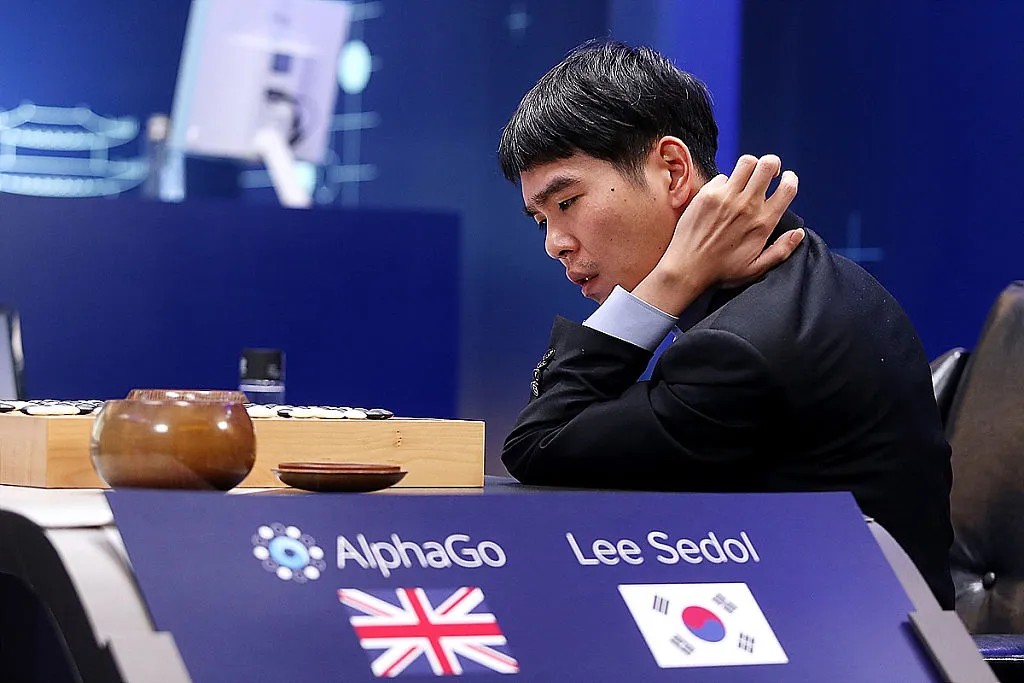
\includegraphics[width=.7\textwidth]{Figures/go-lee-sedol.png}
	\caption{Lee Sedol analysant le tablier après sa première victoire du match}
	\label{fig:LeeSedolVsAlphaGo}
\end{figure}
\FloatBarrier
\subsection{Le coût de l'IA}
Cette explosion de l'IA a causé une explosion dans les coûts de leurs entraînement, déploiement et fonctionnement.


\subsubsection{Le coût économique}
Les modèles d'intelligences artificielles les plus robustes nécessitent des ressources énormes pour leur entraînement et même fonctionnement.
\newline En effet: 
\begin{itemize}
	\item L'entraînement de AlphaGo Zero a coûté approximativement 25 millions de dollars \cite{AlphaGoZeroCost}.
	\item L'entraînement de NAS a coûté approximativement 3 millions de dollars \cite{ShrinkingDeepLearningCarbon}.
\end{itemize}
\subsubsection{Le coût énergitique}
L'utilisation gigantesque des ressources causent une consommation énorme d'énergie.
\newline Par exemple:
\begin{itemize}
	\item Dans le match contre Lee Sedol, AlphaGo a utilisé 1202 GPUs et 176 CPUs. Une estimation de la puissance consommé montre un chiffre colossal de $1$ mégawatts \cite{ShrinkingDeepLearningCarbon}.
	\item Pour entraîner NAS, l'énergie totale consommée est estimée à $656347 \ \text{kWh}$ \cite{CO2Footprint}.
\end{itemize}
\subsubsection{Le coût environmental}
Le coût environmental des modèles IA avancés est souvent très importants. 
\newline En effet, les estimations de $\text{CO}_2$ générés par ces algorithmes peut dépasser l'ordre de milliers de kilogrammes:
\begin{itemize}
	\item 
\end{itemize}
\begin{table}[ht]
	\small
	\centering
	\begin{tabularx}{\textwidth}{| p{3cm} | X | X | p{2cm} | p{2.2cm} | p{3cm} |}
		\hline
		Modèle / Objet & Hardware & Puissance (Watt) & Temps de fonctionnement (Heures) & $\text{CO}_2$ équivalents (kg) & Budget cloud (dollars américains) \\
		\hline 
		Transformer\textsubscript{base} & P100x8 & 1415.78 & 12 & 11.79 & \$41 - \$410 \\
		\hline
		Transformer\textsubscript{big} & P100x8 & 1515.43 & 84 & 87.08 & \$289 - \$981 \\
		\hline
		ELMo & P100x3 & 1415.78 & 12 & 11.79 & \$433 - \$1472 \\
		\hline
		BERT\textsubscript{base} & V100x64 & 12041.51 & 79 & 652.27 & \$3751 - \$12571 \\ 
		\hline
		NAS & P100x8 & 1515.43 & 274120 & 284019 & \$942973 - \$3201722 \\
		\hline
		AlphaGo & & $\approx 1000000$ & 960 & 96000 & $\approx \$250000000$ \\ 
		\hline
		Climatiseur& & 840 &  &  & \\
		\hline
		Refrégirateur & & 1233 & & & \\
		\hline
		Avion SF $\rightarrow$ NY  & & & & 900 & \\
		\hline
		Personne durant 1 an & & & & 5000 & \\
		\hline
		Voiture durant sa vie & & & & 57152 & \\
		\hline
		Maison durant son construction \cite{HouseCarbonFootprint} & & & & 50000 - 80000 &  \\
		\hline
	\end{tabularx}
	\caption{Coût des modèles de IA.}
	\label{table:EnergyConsumption}
	
\end{table}
\FloatBarrier
\subsection{Les limites des systèmes embarqués}
\newpage 
\section{Le Binary Neural Network}
\subsection{Introduction}
\subsection{La signification de "Binary"}
\newpage 
\section{BinaryFlow}
\subsection{Introduction}
BinaryFlow est une bibliothèque de Deep Learning basée sur Larq et TensorFlow
\subsection{Raison d'exister}
\subsection{Signification du nom}
Le choix de nom "BinaryFlow" est influencé de nom "TensorFlow" de la fameuse bibliothèque d'apprentissage automatique et de programmation différentielle qui est crée et maintenue par Google.
\newline TensorFlow se traduit en "flux de tenseurs" qui est l'utilisation excessive  des tenseurs - qui sont grosso modo des tableaux numériques multidimensionnels - dans les calculs différentiels.
\newline Par analogie, BinaryFlow se traduit en "flux binaire" qui signifie l'utilisation excessive des opérations booléennes sur des tenseurs binaires.
\subsection{Solutions offertes par BinaryFlow}
\subsubsection{Couches}
BinaryFlow supporte toutes les couches offertes par TensorFlow et Larq. Mais il aussi supporte:
\begin{itemize}
	\item BinaryNet: Dense, ConvND, TransposedConvND, SeparableConvND.
	\item XnorNet: Dense, ConvND.
	\item XnorNet++: Dense, ConvND.
	\item ABCNet: Dense, Conv1D, Conv2D, Conv3D
	\item BiRealNet: Dense, Conv1D, Conv2D, Conv3D
	\item MeliusNet: Dense, Conv1D, Conv2D, Conv3D
\end{itemize}
\subsubsection{Binarisations}
BinaryFlow supporte toutes les binarisations standard offertes par Larq, et les étend en ajoutant:
\begin{itemize}
	\item Binarisation décalée: qui est une méta-binarisation, qui prend une binarisation $\Psi$ et donne $\Psi_\mu=x\rightarrow \Psi(x+\mu)$ avec $\mu \in\mathbb{R}$ entraînable
	\item Binarisation stochastique: qui est une méta-binaristation qui prend une distribution de probabilité réelle $\mathcal{D}$ en paramètre, et une binarisation $\Psi$, et donne la fonction: $x\rightarrow  \Psi(x-z)$ avec $z\sim U$
	\item Binarisation stochastique décalée
	
\end{itemize}
\subsubsection{Optimiseurs}
BinaryFlow offre les optimiseurs suivants
\begin{itemize}
	\item SGD
	\item Adam\cite{AdamOptimizer}
	\item Bob\cite{BopOptimizer}
\end{itemize}
\subsubsection{Déploiement}
BinaryFlow conserve tous les optimisations offerte par Larq
\chapter{Approche Théorique}
\section{Introduction}

In this chapter we will start by presenting the used paradigms and approaches, the global domain Diagram used in the analysis phase. And then we will explain the different components and their behavior.

\section{Formalisation}\cite{4}
Le BNN, bien que son objectif est clair, elle n'a pas d'approche triviale pour arriver à un réseau "binaire". Pour cela, on va tout d'abord formaliser notre objectif, est après ça, on va essayer de définir un BNN

\subsection{Notations}
Pour simplifier, nous allons commencer par la terminologie des réseaux à perceptrons multicouches.
\pagebreak
\subsubsection{Observations}\label{Theoretical:Observations}
\begin{table}[ht]
	\centering
	\begin{tabularx}{\textwidth}{| X | X |}
		\hline
		$r$ & nombre d'exemplaires du jeux de données \\ 
		\hline
		$\boldsymbol{X}^{\{k\}}$ & l'entrée du $k^\text{ème}$ exemplaire \\
		\hline
		$\boldsymbol{X}=\left(\boldsymbol{X}^{\{1\}},\dots, \boldsymbol{X}^{\{r\}}\right)$ & le tenseur des entrées \\
		\hline
		$\boldsymbol{Y}=\left(\boldsymbol{Y}^{\{1\}},\dots, \boldsymbol{Y}^{\{r\}}\right)$ & le tenseur des résultats \\
		\hline
		$\boldsymbol{U}=\left(\boldsymbol{U}^{\{1\}},\dots, \boldsymbol{U}^{\{r\}}\right)$ & le tenseur des observations \\
		\hline
		
		$\hat{\boldsymbol{Y}}$                    & Une estimation de $\boldsymbol{Y}$      \\ 
		\hline 
		$\mathcal{L}$                    & Une fonction objective      \\ 
		\hline 
		$\mathcal{L}(\hat{\boldsymbol{Y}},\boldsymbol{Y})$                    & L'erreur d'estimation de $Y$       \\ 
		\hline 
	\end{tabularx}
	\caption{Terminologie des jeux de données}
	\label{table:Datasets}

\end{table}

\subsubsection{Division en Lots}
\begin{table}[ht]
	\centering
	\begin{tabularx}{\textwidth}{| X | X |}
		\hline
		$m$ & nombre de lots \\ 
		\hline
		$s_k$ & la taille du $k^\text{ème}$ lot \\
		\hline
		$\boldsymbol{X}^{[k]}$ & le $k^\text{ème}$ lot d'entrées \\
		\hline
		$\boldsymbol{Y}^{[k]}$ & le $k^\text{ème}$ lot de sorties \\
		\hline
		$\boldsymbol{U}^{[k]}$ & le $k^\text{ème}$ lot des observation \\ 
		\hline
		
		$\mathcal{L}(\hat{\boldsymbol{Y}}^{[k]},\boldsymbol{Y}^{[k]})$                    & l'erreur d'estimation de $k^\text{ème}$ lot       \\ 
		\hline 
		
	\end{tabularx}
	\caption{Terminologie de la division en Lots}
	\label{table:Batch}
\end{table}
\begin{remark}
	Par défaut, on va diviser les lots en une taille fixe $s$. \newline
	Comme une exception, le dernier lot va avoir le reste de cette division
\end{remark}
\FloatBarrier
\newpage

\subsubsection{MLP et CNN}
\begin{table}[ht]
	\centering
	\begin{tabularx}{\textwidth}{| X | X |}
		
		\hline
		$\mathcal{N}$          & Un réseau de neurones \\ 
		\hline
		$\mathcal{N}_{\boldsymbol{W}}$          & Un réseau de neurones définit par le tenseur $\boldsymbol{W}$      \\ \hline
		$\boldsymbol{W}^{(l)}$          & La matrice de liaison de la $l^\text{ème}$ couche         \\
		\hline
		$\sigma^{(l)}$& la fonction d'activation de la $l^\text{ème}$ couche \\
				\hline
		$z^{(l)}=\boldsymbol{W}^{(l)}\star a^{(l-1)}$ & le contenu de la couche $l$ avant l'activation\\
		\hline
		$a^{(l)}=\sigma^{(l)}({z^{(l)}})=\sigma^{(l)}(\boldsymbol{W}^{(l)}\star a^{(l-1)})$ & le contenu de la couche $l$ après l'activation \\
		\hline
		$W^{(l)}_{i,j}$                 & le poids de neurone $a^{(l-1)}_{j}$ dans la $i^\text{ème}$ neurones avant l'activation           \\ \hline
		$x=a^{(0)}$                    & L'entrée du réseau de neurones          \\ \hline
		$\hat{y}=a^{(l)}=\mathcal{N}_{\boldsymbol{W}}(x)$              & La sortie du réseau de neurones  \\ \hline
		$n_l$ & le nombre de neurones de la $l^\text{ème}$ couche \\ 
		 \hline 
		
	\end{tabularx}
	\caption{Different machines characteristics}
	\label{table:AcyclicNeuralNetwork}
	\begin{remark}
		Le terme $W^{(l)} \star a^{(l-1)}$ est  interprété comme:
		\begin{enumerate}
			\item une multiplication matricielle $W^{(l)}\cdot a^{(l-1)}$ dans le cas d'une couche dense
			\item une opération de convolution $W^{(l)}* a^{(l-1)}$ dans le cas d'une couche convolutionelle
		\end{enumerate}
		 
	\end{remark}
\end{table}
\FloatBarrier


\subsection{Définition d'un BNN}
Avant de définir un BNN, nous allons introduire le concept des binarisations et des quantifications:
\begin{definition}
	Une binarisation est une fonction $\Psi:\mathbb{R}\rightarrow \mathcal{B}$ avec $\mathcal{B}$ un ensemble à deux éléments.
	\newline Dans le cas d'un tenseur, la binarisation est appliquée élément par élément.
	\newline On va distinguer essentiellement deux valeurs particulières de $\mathcal{B}:$
	\begin{itemize}
		\item $\mathcal{B}=\{\pm 1\}$
		\item $\mathcal{B}=\{0,1\}$
	\end{itemize}
\end{definition}
\begin{definition}
	Un scalaire $u$ est dit binarisé s'il varie dans un ensemble $\mathcal{B}$ à deux éléments.
	\newline Un tenseur de rang $r$ et de dimension $n_1\times\dots\times n_r$ est dit binarisé s'il varie dans un ensemble $\mathcal{B}^{n_1\times\dots\times n_r}$ avec $\mathcal{B}$ à deux éléments.
\end{definition}
\begin{definition}
	Une quantification est un opérateur $\Psi$ appliqué à un tenseur juste avant l'opération bilinéaire en conservant ses dimensions.
\end{definition}
\begin{remark}
	Dans les réseaux de neurones classiques, il n'y a pas de quantifications. En faite, l'absense d'une quantification est équivalente à l'utilisation de la quantification $\mathtt{id}:x\rightarrow x$
\end{remark}

\subsubsection{Dans la littérature}
Le BNN n'admet pas d'une définition unique. En contre partie, dans la littérature\cite{BNNDefinition}, la plupart des réseaux sont nommées binaires puisque :
\begin{enumerate}
	\item Pour chaque paire de nœuds connexe $(u,v).$ Le poids de la liaison est $\omega(u,v)=\pm 1$
	\item Pour chaque couche cachée, la fonction d'activation est la fonction signe $\sign$
\end{enumerate}
\subsubsection{Notre définition}
Nous avons proposé cette définition pour essaier d'unifier les approches des BNNs:
\begin{definition}
Un BNN est tout réseau de neurones admettant au moins une couche dont les quantifications sont des binarisations
\newline Un BNN idéal est un réseau de neurones dont toutes les quantifications sont des binarisations
\end{definition}
\begin{remark}
	Dans ce stage, nous allons concentrer sur les binarisations dont $\mathcal{B}=\{\pm 1\},$ et surtout la binarisation $\sign$
\end{remark}
\begin{remark}
	Bien que la définition est un peu permissive, nous n'allons considérer que les BNNs qui on un nombre "important"\footnote{Grosso modo, le nombre de binarisations doit être aussi important pour justifier les apports des binarisations.} de binarisations.
\end{remark}
\subsection{Objectif}
\subsubsection{Notations}
\begin{itemize}
\item Soit $\mathcal{D}=\left(\boldsymbol{X},\boldsymbol{Y}\right)$ le jeu de données
\item Soit $\mathcal{N}_{\boldsymbol{W}}$ un réseau de neurones admettant le tenseur de paramètres $\boldsymbol{W}.$ 
\end{itemize}
\subsubsection{Problème d'optimisation}
 L'objectif "idéal" est la résolution du problème d'optimisation suivant:
\begin{equation}\label{ObjectiveFunction}
	\boldsymbol{W}^*=\argmin_{\boldsymbol{W}} \mathcal{L}\left(\mathcal{N}_{\boldsymbol{W}}(\boldsymbol{X}),\boldsymbol{Y}\right)
\end{equation}
L'objectif pour un BNN est aussi la minimisation de \eqref{ObjectiveFunction}, mais la seule différence est que le réseau admet des binarisations comme quantifications.
\newpage


\section{Entraînement}

Notre définition de BNN pose beaucoup de problème dans l'entraînement, dont la résolution exige des approches sophistiquées.

\subsection{Difficulté du problème discret}
Soit $\mathcal{N}$ un réseau de neurones binaire idéal ayant une topologie fixe, et soit $\eta$ le nombre total de ses paramètres binarisés. 
\newline Dans le plus mauvais cas, la complexité de trouver les valeurs optimales des paramètres pour ce réseau est  $\mathcal{O}(2^\eta)$ qui n'est pas du tout pratique.

Deux solutions se présentent:
\begin{enumerate}
	\item Approcher le problème discret avec des algorithmes d'approximations et des heuristiques.
	\item Retourner à l'optimisation continue de la fonction objective, 
\end{enumerate}


\subsection{Gradient Nul}
Nous allons opter pour la deuxième solution dans ce stage. Mais, malheureusement, on ne peut pas appliquer directement les méthodes d'optimisations de premier ordre, ou même d'ordre supérieur.
\newline Le problème majeur provient de la lemme suivante:
 \begin{lemma}
 	Toute binarisation continue presque partout\footnote{Le mot "presque partout" est interpreté au sens de la théorie des mesures, et précisément la mesure naturelle dans $\mathbb{R}$ (mesure de Leibniz). Par exemple, dans un sens, la "dérivée" de la fonction $\sign$ est la fonction de Dirac $\delta$} admet une dérivée nulle presque partout
 \end{lemma}
\begin{proof}
	Soit $\Phi:\mathbb{R}\rightarrow \{a_0,a_1\}$ une binarisation continue partout sauf un ensemble $\mathcal{D}$ de mesure nulle, avec $a_0,a_1\in\mathbb{R}$ et $a_0\neq a_1.$
	\newline Soit $x_0\in\mathbb{R}$ tels que $\Phi$ est continue en $x_0,$ et soit $0 <\epsilon < \lvert a_1 -a_0 \rvert$ et $\delta\in\mathbb{R}_+^*$ tel que $$x\in\mathscr{B}(x_0,\delta)\implies \lvert \Phi(x)- \Phi(x_0)\rvert < \epsilon$$
	On a nécessairement, $\Phi(\mathscr{B}(x_0,\epsilon))= \{a_i\}$ avec $i\in\{0,1\}$, et donc $\Phi$ est constante sur $\mathscr{B}(x_0,\delta),$ et ainsi dérivable sur cet interval et en particulier en $x_0$, et on a: 
	$$
	\Phi'(x_0)=0
	$$
	Ainsi:
	$$
	\forall x\in\mathbb{R},\quad \Phi \ \text{continue en} \ x \implies \Phi \ \text{dérivable en} \ x \ \text{et}\ \Phi'(x)=0  
	$$
	Finalement, on a $\Phi$ est continue sur $\mathcal{S}=\mathbb{R}\setminus\mathcal{D}$, avec $\mathcal{D}$ est de mesure nulle, et donc $\Phi$ est dérivable sur $\mathcal{S}$  et par conséquent $\Phi'=0$ sur $\mathcal{S} \ \blacksquare$
\end{proof}
Cette lemme pause un problème puisque la mise à jour des paramètres sera impossible avec des gradient nuls presque partout.
\newline 
Pour résoudre ce problème, nous pouvons:
\begin{enumerate}
	\item Faire une approximation de la binarisation par une fonction plus régulière, surtout dans la propagation en arrière.
	\item Faire une relaxation concernant la notion de gradient à l'aide d'un opérateur $\mathcal{G}$ adéquat "avec lequel on peut appliquer les méthodes de premier ordre.
\end{enumerate} 
Dans le chapitre suivant, nous allons voir chacune des approches 1 et 2.
\begin{figure}[htp!]
	\centering
	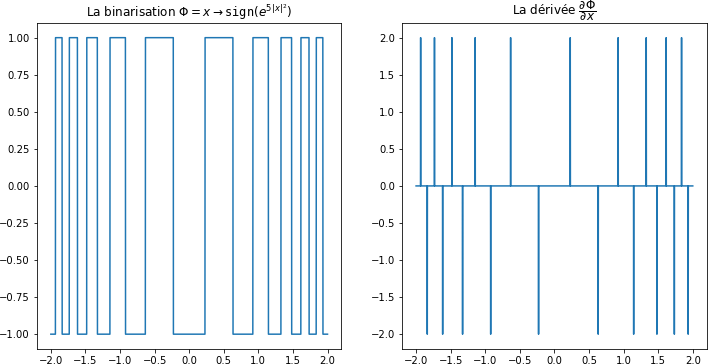
\includegraphics[width=.75\textwidth]{Figures/binarisation-plot.png}
	\caption{Un exemple d'une binarisation et sa dérivée}
	\label{fig:Binarisation-Example}
\end{figure}
\FloatBarrier
\newpage
\section{Optimisations}
\subsection{Définitions}
On note par:

\begin{itemize}
\item $(\mathbb{B},+,\cdot,\bar{},0,1 )$ une algèbre de boole.
\item l'opérateur $\mathtt{XOR}$ par $\oplus$ défini par:
\newline $a\oplus b = \mathtt{XOR}(a,b)=a\cdot \bar{b}+\bar{a}\cdot b=\bar{a}\oplus \bar{b}$
\item l'opérateur $\mathtt{XNOR}$ par $\odot$ défini par:
\newline $a\odot b = \mathtt{XNOR}(a,b)=\overbar{\mathtt{XOR}(a,b)}= (a + \bar{b}) (\bar{a}+b) = a\cdot b + \bar{a} \cdot \bar{b}=\bar{a}\odot \bar{b}$
\end{itemize}

\subsection{Codage sur $1\text{bit}$}
Puisque les poids et noeuds des couches cachées sont tous binarisés, on peut coder chaque valeur sur un seul bit. Ainsi on peut introduire le codage: 
$$\Psi: \begin{cases}
	-1 & \rightarrow 0 \\
	1 & \rightarrow 1
\end{cases}$$

En faite, on regroupe chaque $8$ variables dans la même case mémoire.

\subsection{Utilisation de $\mathtt{XNOR}$}
\subsubsection{Transformation de $\times$ en $\mathtt{XNOR}$}
Dans le cas d'un BNN, les noeuds et les poids sont binarisés. Ainsi toute multiplication est entre deux éléments de $\{-1,1\}.$
\newline Or, par la transformation bijective: 
$$\Psi:\begin{cases}
	1 &\rightarrow 1 \\
	-1 &\rightarrow 0
	\end{cases}$$
On a l'égalité suivante:
$$
\forall a,b\in\{-1,1\},\quad \Psi(a\times b) = \Psi(a)\odot \Psi(b) 
$$
\begin{figure}[h!]
	\centering
	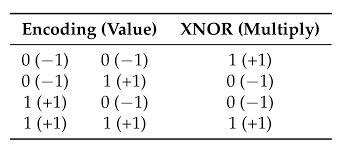
\includegraphics[width=.5\textwidth]{Figures/XNOR-Table.png}
	\caption{Table de multiplication en utilisant XNOR}
	\label{fig:XNOR-Table}
\end{figure}
\FloatBarrier
\begin{proof}
	On a le groupe $(\mathbb{C}_2,\times )$  avec $\mathbb{C}_2=\{z\in \mathbb{C} / \quad z^2=1\}=\{-1,1\}$ est cyclique et d'ordre $2.$ Ainsi, il est isomorphe au groupe $(\mathbb{F}_2,\oplus)$ où $\mathbb{F}_2=\mathbb{Z}/2\mathbb{Z}=\{0,1\},$ et $\oplus$ est l'addition modulo $2$. 
	\newline L'ismorphisme entre eux est: 
	$$\Psi_1=\begin{cases}
		-1 & \rightarrow 1 \\
		1 & \rightarrow 0
	\end{cases}$$
	De plus, le corps $(\mathbb{F}_2,\oplus,\times)$ induit l'algèbre de boole $(\mathbb{F}_2,+,\times,\bar{},0,1)$ avec:
	\begin{align*}
		\bar{a}&=a\oplus 1 \\
		a+ b &= \overbar{\bar{a}\times\bar{b}}
	\end{align*}
	Or, par dualité de l'algèbre booléenne, l'opérateur de négation $\Psi_2:a\rightarrow \bar{a}$ est un isomorphisme entre $(\mathbb{F}_2,+,\times,\bar{},0,1)$ et $(\mathbb{F}_2,\times,+,\bar{},1,0)$
	
	Ainsi on a:
	\begin{align*}
	\forall a,b\in\{-1,1\}, \quad \Psi_2\circ \Psi_1( a\times b)  &= \Psi_2(\Psi_1(a\times b)) \\
			&=\Psi_2(\Psi_1(a)\oplus \Psi_1(b)) \ \text{isomorphisme 1} \\ 
			&=\overbar{\Psi_1(a)\oplus \Psi_1(b)}  \\
			&=\Psi_1 (a) \odot \Psi_1(b) \ \text{isomorphisme 2} \\
			&= \overbar{\Psi_1 (a)} \odot \overbar{\Psi_1(b)} \\
			&= \Psi_2\circ \Psi_1 (a) \odot \Psi_2\circ \Psi_1(b)  
	\end{align*}
	Maintenant, il ne reste qu'à vérifier que $\Psi=\Psi_2\circ \Psi_1:$
	\begin{align*}
		\Psi_2\circ \Psi_1(-1) &=\Psi_2(\Psi_1(-1))\\
		&=\Psi_2(1) \\
		&=0 \\
		\Psi_2\circ \Psi_1(1) &=\Psi_2(\Psi_1(1))\\
		&=\Psi_2(0) \\
		&=1 \quad \blacksquare
	\end{align*}
\end{proof}
\subsubsection{Avantages}
En faite, dans les circuits intégrés, l'opération $\mathtt{XNOR}$ est plus rapide que $\times$. En faite, elle:
\begin{itemize}
	\item consomme moins d'énergie
	\item peut être faite $32$ fois dans un seul cycle. Par comparaison, une seule opération $\times$ peut dépasser $1$ cycle 
\end{itemize}
 \newpage
\subsection{Utilisation de $\mathtt{POPCOUNT}$}
	\subsubsection{Définition de $\mathtt{POPCOUNT}$}
	$\mathtt{POPCOUNT}$ est une instruction qui permet de compter les bits qui sont mis à $1$ dans un vecteur de bits $v.$
	\begin{remark}
		$v$ peut être la représentation binaire d'un nombre $n$
	\end{remark} 
	\subsubsection{Produit scalaire de deux vecteurs binarisés}
	Soit $u,v\in\{-1,1\}^n.$ On a:
	\begin{align*}
		\langle u,v \rangle &=\sum_{i=1}^n u_iv_i \\ 
		&=  \sum_{i=1}^n \Psi^{-1}(\Psi(u_i)\odot\Psi (v_i)) \\
		&= \mathtt{POPCOUNT}(\Psi(u)\odot \Psi(v)) \cdot \Psi^{-1}(1) + \left(n-\mathtt{POPCOUNT}(\Psi(u)\odot \Psi(v))\right)\cdot \Psi^{-1}(0) \\
		&= \mathtt{POPCOUNT}(\Psi(u)\odot \Psi(v))-\left(n-\mathtt{POPCOUNT}\left(\Psi(u)\odot \Psi(v)\right)\right) \\
		&= 2\cdot \mathtt{POPCOUNT}(\Psi(u)\odot \Psi(v)) - n \\
		&= \left(\mathtt{POPCOUNT}\left(\Psi(u)\odot \Psi(v)\right) \ll 1 \right) - n
	\end{align*}
	\begin{figure}[h!]
		\centering
		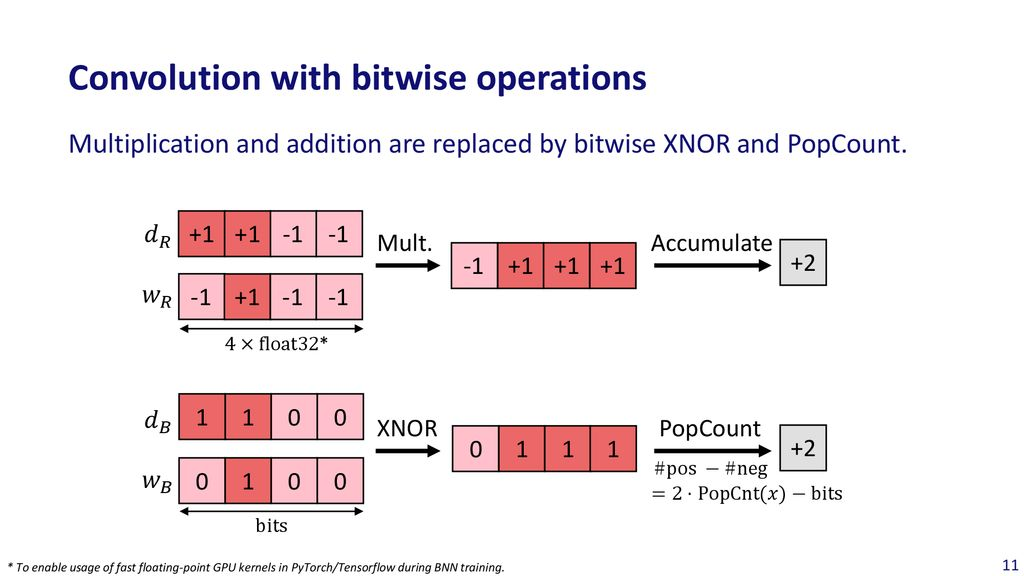
\includegraphics[width=.9\textwidth]{Figures/POPCOUNT.jpg}
		\caption{Calcul du produit scalaires}
		\label{fig:POPCOUNT}
	\end{figure}
\pagebreak
	\subsubsection{Estimation de coût}
	 On suppose pour $m\in \mathbb{N}^*$, que notre processeur supporte dans une seule instruction, un $\mathtt{XNOR}$ bit-wise des deux vecteurs bits $u,v\in\{0,1\}^m$  
	\newline On suppose aussi pour cette même valeur de $m$ que notre processeur supporte dans une seule instruction, un $\mathtt{POPCOUNT}$ bit-wise d'un vecteur bits $u\in\{0,1\}^m$  
	\newline Soit $n=mr, \ r\in\mathbb{N}^*,$ et soit $u,v\in\{-1,1\}^n$ 
	\newline Pour $p\in\{1,r\},$ soit: 
	$$\begin{cases}
		u^{[p]}=(u_{(p-1)m+1},\dots u_{pm}) \\ v^{[p]}=(v_{(p-1)m+1},\dots v_{pm})
		\end{cases}$$
	On a:
	\begin{align*}
		\langle u ,v\rangle &= \sum_{i=1}^{n} u_iv_i\\
		&= \sum_{p=1}^r \langle u^{[p]},v^{[p]}  \rangle \\
		&= \sum_{p=1}^r 2\cdot \mathtt{POPCOUNT}\left(\Psi\left(u^{[p]}\right) \odot \Psi\left(v^{[p]}\right)\right) - m \\
		&= 2\sum_{p=1}^r  \mathtt{POPCOUNT}\left(\Psi\left(u^{[p]}\right) \odot \Psi\left(v^{[p]}\right)\right) - \sum_{p=1}^r m \\
		&= \left( \sum_{p=1}^r  \mathtt{POPCOUNT}\left(\Psi\left(u^{[p]}\right) \odot \Psi\left(v^{[p]}\right)\right)  \ll 1\right)-n
	\end{align*}

	Ainsi, on a optimisé $n$ multiplications et $n-1$ additions en:
	\begin{itemize}
		\item $r-1=\frac{n}{m}-1$ additions.
		\item $r$ instructions $\mathtt{XNOR}$
		\item $1$ décalage à gauche.
		\item $1$ soustraction.
	\end{itemize} 
\pagebreak
\subsection{Gain Temps \& Mémoire}
\subsubsection{Gain Mémoire}
Les implémentations classiques des RN utilisent des paramètres en firgules flottantes à precision simple. c'est à dire chaque paramètre prends $32 \ \text{bits}.$
\newline Avec le codage considéré, on peut avoir un gain de mémoire $\alpha_{\text{mémoire}}=32$

\subsubsection{Gain Temps}
Le gain de l'opération de produit scalaire est:
\begin{align*}
\alpha_{\langle \cdot , \cdot \rangle} &= \frac{n+n-1}{\frac{n}{m}-1+\frac{n}{m}+1+1}  \\
&= \frac{2n-1}{2\frac{n}{m}+1} \\
&= \frac{2-\frac{1}{n}}{2\frac{1}{m}+\frac{1}{n}} \\
&= \frac{2m-\frac{m}{n}}{2+\frac{m}{n}} \\
&= \frac{m-\frac{m}{2n}}{1+\frac{m}{2n}}\\
&= m -\frac{m(m+1)}{2n} + o\left(\frac{m^3}{n^2}\right)
\end{align*}

On a:
\begin{itemize}
	\item Pour un PC personnel, ou même téléphone: $m=64.$
	\item Pour les réseaux de neurones standards, $32\leq n\leq 1024$
\end{itemize}

Ainsi une estimation de $\alpha_{\text{temps}}$ est :
$$
31.5\leq \alpha_{\text{temps}} \leq \frac{2047}{32} \approx 62.03
$$ 
\chapter{Modélisation}

\section{Introduction}

Dans ce chapitre, on va étudier les approches faites dans la conception et implémentation des réseaux de neurones binaires,  dériver les formules nécessaires dans les cas des couches dense et convolutionnelles, et dans le cas générique.

\subsection{Importance de ce chapitre}
Dans les articles de BNNs considérés, les formules données ne sont généralement applicable qu'aux couches convolutionnelles à $2$ dimensions.
\newline Nous chercherons ici à trouver une approche générique avec laquelle on peut dériver pour chaque modèle considéré les équations des couches dense, convolutionnelles, récurrentes, etc...
\newline Notre approche admet principalement $2$ caractéristiques:
\subsubsection{Rigueur}
Pour établir les équations nécessaires, nous avons suivi les étapes suivantes:
\begin{enumerate}
	\item Définir l'utilité potentielle du modèle
	\item Traduire l'objectif en un problème d'optimisation mathématique
	\item Définir les hypothèses nécessaires
	\item Etablir les formules
\end{enumerate}
\subsubsection{Flexibilité}
Grâce au niveau de rigueur utilisé, on peut facilement modifier et même améliorer les équations.
\newline Dans notre implémentation de chaque modèle, nous allons se baser sur les formules de ce chapitre en offrant la possibilité de faire quelques modifications.

\subsection{Convention Utilisée}
Dans les démonstrations, nous allons suivre les conventions mathématiques de l'algèbre linéaire et de l'optimisation mathématique. Mais dans les implémentations, nous allons suivre les conventions de TensorFlow.

\newpage
\section{Histoire}
\begin{table}[h]
	\small
	\begin{tabularx}{\textwidth}{| p{2.5cm} | p{1cm} | X |}
		\hline
		
		Modèle & Année & Idée(s)  \\
		\hline 
		BinaryConnect\cite{BinaryConnectPaper} & 2015 & \begin{itemize}
			\item Binarisation des poids en $\pm 1$
			\item Optimisation des instructions MAC\footnote{Multiply \& Accumulate} en des sommes.
			\item Estimateur direct du gradient pour résoudre le problème d'annulation de gradient.
		\end{itemize}\\
		\hline
		BinaryNet\cite{BinaryNetPaper} & 2015 & \begin{itemize}
			\item Binarisation des paramètres et noeuds en $\pm 1$
			\item Optimisation des instructions MAC\footnote{Multiply \& Accumulate} en des $\mathtt{XNOR}$ et $\mathtt{POPCOUNT}$.
		\end{itemize} \\
		\hline  
		XNOR-NET\cite{XnorNetPaper} & 2016 &  Introduction de deux facteurs $\alpha$ et $\beta$ à chaque produit scalaire pour minimiser l'erreur de l'opérateur bilinéaire $\star$  \\
		\hline
		ABCNet\cite{ABCNetPaper} & 2017 &  \begin{itemize}
			\item Utilisation de $n\in\mathbb{N}^*$ binarisations pour les paramètres: $\widetilde{\boldsymbol{W}}^{(l),1},\dots,\widetilde{\boldsymbol{W}}^{(l),n}$
			\item Utilisation de $m\in\mathbb{N}^*$ binarisations pour les noeuds: $\tilde{a}^{(l),1},\dots,\tilde{a}^{(l),m}$
			\item Décomposition de l'opération bilinéaire $\boldsymbol{W}^{(l)}\star a^{(l-1)}$ en une combinaison linéaire des $\widetilde{\boldsymbol{W}}^{(l),i} \star\tilde{a}^{(l-1),j} $ pour $i\in\{1,\dots,n\}$ et $j\in\{1,\dots,m\}$ 
		\end{itemize}\\
		\hline
		BiRealNet\cite{BiRealNetPaper} & 2019 & \begin{itemize}
			\item Ajout d'une architecture résiduale
			\item Approximation régulière plus fine de la fonction $\sign$
		\end{itemize}\\
		\hline
		MeliusNet & 2020 & \begin{itemize}
			\item Utilisation des blocs denses pour augmenter la capacité des caractéristiques 
			\item Utilisation des blocs d'améliorations pour augmenter la qualité des caratéristiques
		\end{itemize}\\
		\hline 
	\end{tabularx}
	\caption{Le tableau d'avancement des BNNs}
\end{table}
\FloatBarrier
\newpage
\section{Comparaison}
\subsection{Par quantification}
\begin{table}[h]
	\small
	\begin{tabularx}{\textwidth}{| p{2.5cm} | X | X |}
		\hline
		
		Modèle & Avantages & Inconvénients(s)  \\
		\hline 
		BinaryNet\cite{BinaryNetPaper} & \begin{itemize}
			\item Le plus léger
			\item Interférence rapide
		\end{itemize} & \begin{itemize}
			\item Induit des modèles très simple.
			\item Admet des mauvaises performances de prédictions pour les tâches difficiles\footcite{En effet, sa performance à ImageNet avec l'architecture ResNet est $27\%$}.
			\item Instable.
		\end{itemize} \\
		\hline  
		XNOR-NET\cite{XnorNetPaper} & \begin{itemize}
			\item Le premier BNN performant.
			\item Interférence rapide.
		\end{itemize} &  \begin{itemize}
		\item Réintroduit des multiplication et divisions.
		\item Performances modestes.
	\end{itemize} \\
		\hline
		ABCNet\cite{ABCNetPaper} &  \begin{itemize}
			\item Très performant.
			\item Il est stable par rapport aux autres.
			\item Admet une justification théorique grâce à l'algèbre linéaire.
		\end{itemize} &  \begin{itemize}
			\item Le temps d’interférence est en $\mathcal{O}(nm)$.
			\item La mémoire est en $\mathcal{O}(n+m)$
		\end{itemize}\\
		\hline
	\end{tabularx}
	\caption{Approches de Quantification}
\end{table}
\FloatBarrier
\subsection{Par architecture}
\begin{table}[h]
	\small
	\begin{tabularx}{\textwidth}{| p{2.5cm} | X | X |}
		\hline
		
		Modèle & Avantages & Inconvénients(s)  \\
		\hline 
		BiRealNet\cite{BiRealNetPaper} & \begin{itemize}
			\item BNN performant
			\item Conserve la rapidité d'interférence.
			\item Modèle plus stable
		\end{itemize} & \begin{itemize}
			\item Conçu spécifiquement pour les architectures convolutionnelles
			\item Instable.
		\end{itemize} \\
		\hline  
		MeliusNet & \begin{itemize}
			\item Plus performant que BiRealNet
			\item Conserve la rapidité d'interférence.
			\item Modèle plus stable
		\end{itemize} & \begin{itemize}
			\item Plus lourds que BiRealNet
			\item Conçu spécifiquement pour les architectures convolutionnelles
		\end{itemize} \\
		\hline
	\end{tabularx}
	\caption{Approches de Quantification}
\end{table}
\FloatBarrier
\newpage
\section{BinaryNet}
\subsection{Conception}
BinaryNet\cite{BinaryNetPaper} est le premier réseau de neurones totalement binaires dans ces couches cachés, c'est à dire tout passage d'une couche caché à une autre se fait par des accumulations de nombres binarisés $(\pm 1).$

Autrement dit, c'est le premier réseau de neurones binaires conforme à notre définition. 
\begin{figure}[h!]
	\centering
	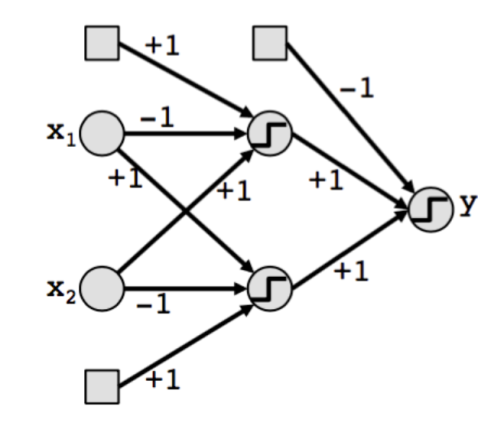
\includegraphics[width=0.5\textwidth]{Figures/BinaryConnect.png}
	\caption{Exemple d'un BinaryConnect à une seule couche cachée}
	\label{fig:BinaryConnect}
\end{figure}
\subsection{Topologie}
BinaryNet est indépendent de l'architecture choisie: Elle peut être dense, convolutionnelle, récurrente, etc\dots 
\newline Mais en pratique, il n'est testé que dans le cas dense et convolutionnel.



\subsection{Utilisation d'Estimateur Direct de gradient}
\subsubsection{Problématique}
Puisque la fonction signe est constante par morceau, son dérivé est donc nulle presque partout (dans le sens de la théorie des mesures).
\newline Ainsi, tout algorithme basé sur le gradient doit mettre en considération
\subsubsection{Principe}
L'entraînement d'un BNN est similaire à un RN classique:
\begin{enumerate}
	\item Une propagation en avant pour calculer la valeur de la fonction objective
	\item Une propagation en arrière pour calculer le gradient des paramètres
	\item La mise à jour des paramètres
	\item Refaire l'étape 1, jusqu'à satisfaire un critère bien déterminé (convergence, dépassement de la limite des époches, taux d'entraînement négligeable, etc...)
\end{enumerate}

L'estimateur direct de gradient\cite{STEPaper} sert à corriger le problème du gradient nul en faisant une estimation plus régulière de la fonction signe dans la propagation arrière (la fonction signe reste toujours utilisée dans la propagation avant)

L'estimation utilisée de la fonction $\sign$ est la fonction $\hardtanh$ définie par:
\begin{align*}
	\hardtanh:& \mathbb{R}\rightarrow \mathbb{R} \\
	&x\rightarrow \begin{cases}
		-1 & \text{si } x < -1 \\
		x & \text{si } \lvert x\rvert \leq 1 \\
		1 & \text{si }  x > 1
	\end{cases}
\end{align*}

En faite son dérivé est:
\begin{align*}
	\forall x \in\mathbb{R},\quad \dfrac{\partial \hardtanh}{\partial x}(x)&=\mathds{1}_{\lvert r \rvert \leq 1}(x)\\
	&=
	\begin{cases}
		1 & \text{si } \lvert x \rvert \leq 1 \\
		0 & \text{sinon}
	\end{cases}
\end{align*}

\begin{figure}[h!]
	\centering
	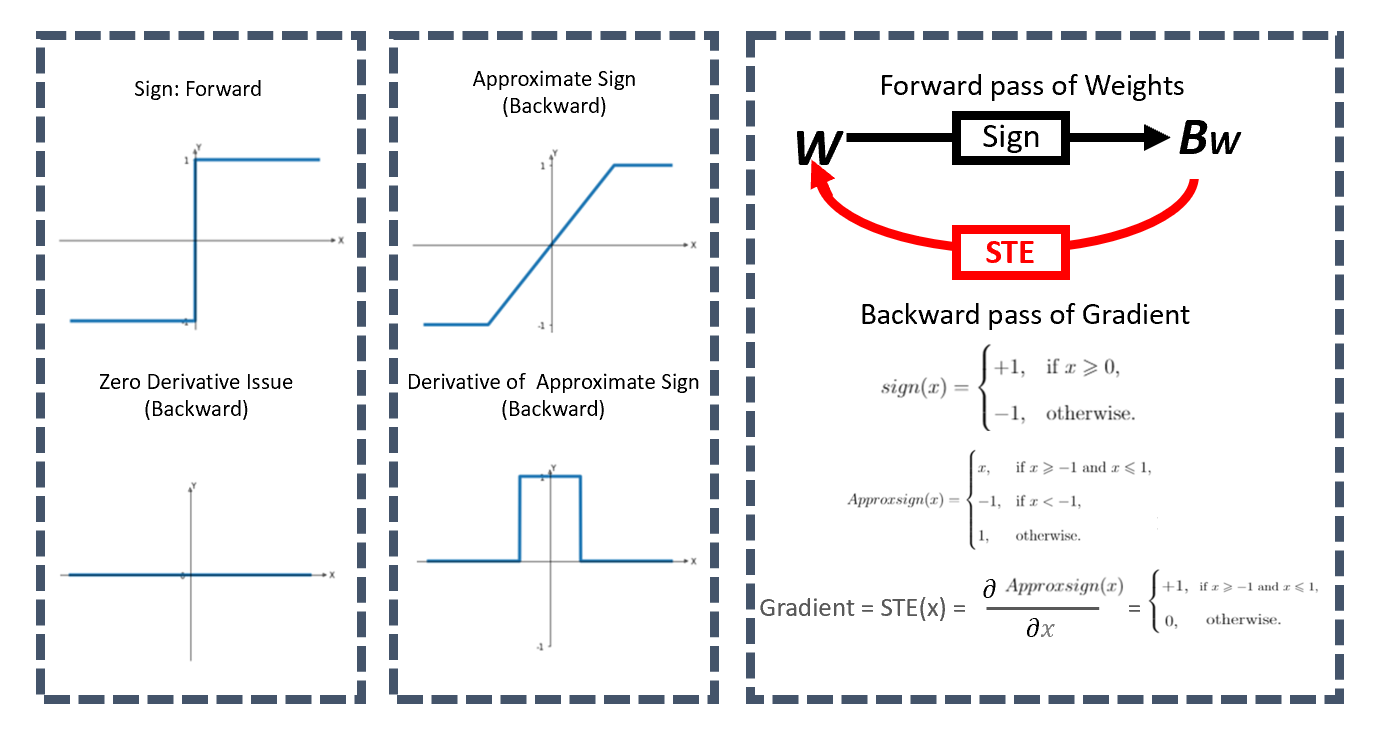
\includegraphics[width=1\textwidth]{Figures/STE.png}
	\caption{Estimateur direct du gradient}
	\label{fig:STE}
\end{figure}
\FloatBarrier

\subsubsection{Estimation du gradient}
Soit $f$ une fonction
Soit $\boldsymbol{x},\boldsymbol{y}$ deux tenseurs tels que $f(\bold{x})=y$ On note par $\mathcal{G}_{\boldsymbol{x}}$ l'estimation de gradient $\dfrac{\partial \mathcal{L}}{\partial \boldsymbol{x}}$ (par la méthode STE) et on la définit par:
$$
\mathcal{G}_{\boldsymbol{x}}=\begin{cases} 
	\dfrac{\partial \mathcal{L}}{\partial \boldsymbol{x}} \odot \mathds{1}_{\lvert \boldsymbol{x} \rvert \leq 1} & \text{si } f=\sign\\
	\mathcal{G}_y \cdot \dfrac{\partial \boldsymbol{y}}{\partial \boldsymbol{x}} & \text{sinon}
\end{cases}
$$

\begin{remark}
	Le calcul de $\mathds{1}_{\lvert \boldsymbol{x} \rvert \leq 1}$ se failt élément par élément. 
\end{remark}
\begin{remark}
	L'opérateur $\odot$ dénote la multiplication élément par élément
\end{remark}

La mise à jour des paramètres se fait en remplaçant chaque gradient par son estimation.

\subsubsection{Justification Théorique}
\subsection{Optimisations possible}
Etant un réseau totalement binarisé dans les couches cachées, BinaryConnect peut avoir plusieurs optimisations, y compris:
\begin{itemize}
	\item Utilisation du Codage binaire
	\item Utilisation des instructions $\mathtt{XNOR}$ est $\mathtt{POPCOUNT}$ pour accélerer la propagation avant
	\item Utilisation de ADA-Max pour accélérer la mise à jour des paramètres
	\item Utilisation de "Shifted Batch Normalisation" pour accélérer le calcul de la normalisation par lots.
\end{itemize}
\newpage

\section{XNOR-NET}
\subsection{Conception}
XNOR-NET\cite{XnorNetPaper} est le premier réseau de neurones binaires admettant des performances acceptables. Il est basé sur BinaryNet, et il met  l'accent sur l'utilisation de $\mathtt{XNOR}$ et $\mathtt{POPCOUNT}$ \cite{XnorNetPaper}.

De plus, Il introduit une nouvelle approche pour réduire l'erreur de quantification



\subsection{Topologie}
Comme BinaryConnect, XNOR-NET\cite{XnorNetPaper} est indépendent de l'architecture et la topologie utilisée.

En autre partie, il n'est pratiquement implémenté que dans les architectures denses et convolutionnelles.

\subsection{Réduction de l'erreur de quantification}
Pour $\boldsymbol{W}^{(l)}$ et $a^{(l-1)},$ on veut trouver deux facteurs $\alpha,\beta \in\mathbb{R}_+,$ et deux binarisations $\tilde{\boldsymbol{W}}^{(l)}$ et $\tilde{a}^{(l-1)}$ respectivement de $\boldsymbol{W}^{(l)}$ et $a^{(l-1)}$ tels que:
\begin{align}
	\boldsymbol{W}^{(l)} & \approx \alpha  \tilde{\boldsymbol{W}}^{(l)} \label{XnorNet:W}\\ 
	 \tilde{a}^{(l-1)} & \approx \beta  \tilde{a}^{(l-1)} \label{XnorNet:a}\\
	 \boldsymbol{W}^{(l)}\star a^{(l-1)} &\approx \alpha \beta  \tilde{\boldsymbol{W}}^{(l)}\star \tilde{a}^{(l-1)} \label{XnorNet:z}
\end{align}

Dans l'objectif décrit, les binarisations ne sont pas nécessairement la fonction $\sign,$ mais on montrera que c'est toujours un bon choix.
\subsection{Quantification optimale d'un vecteur}\label{XnorNet:VectorQuantification}
Dans cette section, nous allons trouvé les paramètres $\alpha$ et $\beta$ optimaux des équation respectifs \eqref{XnorNet:W} et \eqref{XnorNet:a} sans tenir compte de l'équation \eqref{XnorNet:z}.
\newline C'est à dire, nous allons dériver les quantification optimales de $\boldsymbol{W}^{(l)}$ et $a^{(l-1)}$ sans tenir compte de la qualité de la quantification \eqref{XnorNet:z} de $z^{(l)}=\boldsymbol{W}^{(l)}\star a^{(l-1)}.$
\newline En effet, nous allons raisonner d'une manière générale. Et puis les deux résultats vont être immédiatement déduits.

\subsubsection{Notations}
On va dénoter par:
\begin{itemize}
	\item $n\in\mathbb{N}^*$ la dimension de notre espace vectoriel.
	\item  $w$ un vecteur de $\mathbb{R}^n.$
	\item $\tilde{w}\in \{-1,1\}^n$ une binarisation de $w.$
	\item $\gamma\in\mathbb{R}_+$ un facteur d'échelle.
\end{itemize}
\subsubsection{Objectif}
L'objectif est de trouver $\tilde{w}$ et $\gamma$ qui minimisent $\lVert w-\gamma \tilde{w}\rVert_2^2$ pour un $u$ donné:
\begin{equation}\label{XnorNet:VectorQuantification:Problem}
	(\gamma,w)=\argmin_{\gamma,\tilde{w}}\lVert w-\alpha \tilde{w}\rVert_2^2
\end{equation} 
\subsubsection{Résolution du problème}
On a:
\begin{align*}
	\forall \gamma \in \mathbb{R},\forall \tilde w \in \{-1,1\}^n, \quad \lVert w - \gamma\tilde w \rVert_2^2 &= \langle w , w \rangle -2\gamma  \langle w , \tilde w\rangle + \gamma ^2\langle \tilde w , \tilde w \rangle   \\
	&=  \langle w , w \rangle -2\gamma \langle w , \tilde w\rangle + n\gamma ^2 \\
	\text{car }\tilde w \in\{-1,1\}^n,\quad \lVert \tilde w \rVert_2^2 &= \sum_{i=1}^n\tilde w_i^2 = n  
\end{align*}

Maintenant, on a $\langle w,\tilde w \rangle$ est maximisé pour $\tilde w=\sign w,$ et par conséquent puisque $\gamma \ge 0$
\newline $ \langle w , w \rangle -2\gamma \langle w , \tilde w\rangle + n\gamma ^2$ est minimisé pour $\tilde w=\sign w \quad \forall \gamma \in\mathbb{R}_+.$
\newline Ainsi le problème est réduit à la minimisation de la fonction quadratique suivante:
\begin{equation}
	H(\gamma)=\langle w , w \rangle -2\gamma \langle w , \sign w\rangle + n\gamma ^2
\end{equation}

En effet, $H$ étant une fonction convexe sur $\mathbb{R},$ admet un unique minimum local en $x^*=\frac{\langle w,\sign w\rangle}{n}.$
\newline Or, on a:
\begin{align*}
	x^*&=\frac{\langle w,\tilde w \rangle}{n}= \frac{1}{n}\sum_{i=1}^n w_i \sign w_i \\
	&= \frac{1}{n} \sum_{i=1}^n \lvert w_i\rvert = \frac{\lVert w \rVert_1}{n} \ge 0
\end{align*}
Ainsi, $\gamma = x^*$, et donc l'expression de $\gamma$ est:
\begin{equation}
	\gamma = \frac{\lVert w \rVert_1}{n}
\end{equation}

\subsubsection{Quantification de $\boldsymbol{W}^{(l)}$}
On a $\boldsymbol{W}^{(l)} \in E$ où $E\cong \mathbb{R}^{n_1}$ avec $n_1=\dim \boldsymbol{W}^{(l)}.$
\newline Ainsi, on a $\lVert \boldsymbol{W}^{(l)} - \alpha \tilde{\boldsymbol{W}}^{(l)} \rVert_2^2$ est minimisé pour:
\begin{equation}\label{Xnor:W:Expression}
	\begin{cases}
		\alpha &= \frac{\lVert \boldsymbol{W}^{(l)} \rVert }{n_1} \\ 
		\tilde{\boldsymbol{W}}^{(l)} &=\sign \boldsymbol{W}^{(l)}
	\end{cases}
\end{equation}
\subsubsection{Quantification de $a^{(l)}$}
On a $a^{(l)} \in F$ où $F\cong \mathbb{R}^{n_2}$ avec $n_2=\dim a^{(l)}.$
\newline Ainsi, on a $\lVert a^{(l)} - \beta \tilde{a}^{(l)} \rVert_2^2$ est minimisé pour:
\begin{equation}\label{Xnor:a:Expression}
	\begin{cases}
		\beta &= \frac{\lVert a^{(l)} \rVert }{n_2} \\ 
		\tilde{a}^{(l)} &=\sign a^{(l)}
	\end{cases}
\end{equation}

\subsection{Quantification d'un produit scalaire de deux vecteurs}\label{XnorNet:InnerProductQuantification}
Dans cette partie, nous allons tenir compte de la quantification de $z^{(l)},$ c'est à dire nous allons minimiser l'erreur de l'équation \eqref{XnorNet:z}.
\newline La résolution de cette équation n'est pas aussi triviale que \eqref{XnorNet:W}  et \eqref{XnorNet:a}, et donc nous allons majorer l'erreur de quantification $\lVert \langle  u,v \rangle - \langle  \alpha \tilde u,\beta \tilde v \rangle \rVert_2^2$ par une fonction plus facile à optimiser, et nous allons retrouver les expressions \eqref{Xnor:W:Expression} et \eqref{Xnor:a:Expression} de la section précédente.
\subsubsection{Objectif}
\begin{itemize}
\item Soit $n\in\mathbb{N}$ la dimension de l'espace euclidien.
\item Soit $u,v\in\mathbb{R}^n$  
\end{itemize}
Notre objectif est de trouver deux facteurs $\alpha,\beta \in\mathbb{R}_+$ et deux vecteurs $u,v\in\{-1,1\}^n$ qui réduisent $\lVert \langle  u,v \rangle - \langle  \alpha \tilde u,\beta \tilde v \rangle \rVert_2^2$
\subsubsection{Une Borne supérieure de l'erreur}
Une formule exacte pour le problème originale est un peu difficile. Pour cela, on pose $w=u\odot v,$ et on cherche une borne supérieure de $\lVert \langle  u,v \rangle - \langle  \alpha \tilde u,\beta \tilde v \rangle \rVert_2^2$ en fonction de $\lVert w-\alpha\beta \tilde u \odot \tilde v\rVert_2^2$ \cite{XnorNetPaper}:
\begin{align*}
	\lVert \langle  u,v \rangle - \langle  \alpha \tilde u,\beta \tilde v \rangle \rVert_2^2&=(\langle  u,v \rangle - \langle  \alpha \tilde u,\beta \tilde v \rangle)^2 \\
	&= \left(\sum_{i=1}^n u_iv_i-\alpha\beta \tilde u_i \tilde v_i\right)^2 \\
	&= \left\lvert \sum_{i=1}^n\sum_{j=1}^n (u_iv_i-\alpha\beta \tilde u_i\tilde v_i) (u_jv_j-\alpha\beta \tilde u_j\tilde v_j)  \right\rvert \\
	&\leq \sum_{i=1}^n\sum_{j=1}^n \lvert u_iv_i-\alpha\beta \tilde u_i\tilde v_i \rvert  \lvert u_jv_j-\alpha\beta \tilde u_j\tilde v_j \rvert \\
	&\leq \sum_{i=1}^n\sum_{j=1}^n \lVert u\odot v - (\alpha \tilde u) \odot (\beta \tilde v) \rVert_\infty^2\\
	&\leq n^2 \lVert u\odot v - (\alpha \tilde u) \odot (\beta \tilde v) \rVert_\infty^2\\
	&\leq n^2\lVert u\odot v - (\alpha \tilde u) \odot (\beta \tilde v) \rVert_2^2\\
	&\leq  n^2\lVert w - \alpha \beta \tilde u \odot \tilde v \rVert_2^2
\end{align*}

Avec ce résultat, on est sûr qu'en minimisant $\lVert w - \alpha \beta \tilde u \odot \tilde v \rVert_2^2,$ on minimise la borne supérieure de l'erreur de quantification.
\subsubsection{Minimisation de $\lVert w - \alpha \beta \tilde u \odot \tilde v \rVert_2^2$}
En effet, Puisque $\tilde u \odot \tilde v$ génère tout les vecteurs binaires, et $\alpha \beta$ génère tous les réels positifs, on peut trouver $\argmin\limits_{\alpha,\beta,\tilde u ,\tilde v} \lVert w - \alpha \beta \tilde u \odot \tilde v \rVert_2^2$ à partir de $\argmin\limits_{\gamma,\tilde w }\lVert w - \gamma\tilde w \rVert_2^2.$
\newline Or, on a déjà trouvé ce dernier. Ainsi on a:
\begin{equation}
	\begin{cases}
		\tilde u \odot \tilde v = \tilde w=\sign w = \sign u \odot \sign v \\
		\alpha\beta = \gamma = \frac{\lVert w \rVert_1}{n}
	\end{cases}
\end{equation}
\subsubsection{Valeur de $\alpha,\beta,\tilde{u}$ et $\tilde{v}$} 
Pour trouver chacune de $\alpha,\beta$ on fait les hypothèses suivantes:
\begin{itemize}
	\item $u_1,\dots,u_n$ et $\boldsymbol{x}$ suivent une distribution $\mathcal{U}$ à moment absolu de premier ordre fini. 
	\item $v_1,\dots,v_n$ et $\boldsymbol{y}$ suivent une distribution $\mathcal{V}$ à moment absolu de premier ordre fini.
	\item $\forall i,j\in\{1,\dots,n\},\quad u_i \text{ et } v_j \text{ sont indépendents}$ 
	\item $\alpha$ et $\tilde{u}$ ne dépendent que de $u$
	\item $\beta$ et $\tilde{v}$ ne dépend que de $v$
\end{itemize}

En exploitant les hypotèses proposées, on peut facilement trouver $\tilde{u}$ et $\tilde{v}$:
\begin{equation}\label{XnorNet:InnerProductQuantification:Binarisatiosn}
	\begin{cases}
		\tilde{u} = \sign u\\
		\tilde{v} = \sign v
	\end{cases}
\end{equation}
Pour $\alpha$ et $\beta,$ on donne la démonstration suivante:
\begin{align*}
	\mathbb{E}[\gamma] &= \mathbb{E}\left[\frac{\lVert w \rVert_1}{n}\right] = \frac{1}{n}\mathbb{E}\left[\lVert  w \rVert_1\right] \\
	&= \frac{1}{n}\sum_{i=1}^n\mathbb{E}\left[\lvert  u_i v_j \rvert\right] = \frac{1}{n}\sum_{i=1}^n \mathbb{E}\left[\lvert  u_i \rvert]\mathbb{E}[\lvert  v_j \rvert\right] \\
	&= \frac{1}{n}\sum_{i=1}^n \mathbb{E}\left[\lvert  \boldsymbol{x} \rvert\right]\mathbb{E}\left[\lvert \boldsymbol{y} \rvert\right] = \mathbb{E}\left[\lvert  \boldsymbol{x} \rvert\right]\mathbb{E}\left[\lvert \boldsymbol{y} \rvert\right]\\
	&= \mathbb{E}\left[\frac{\lVert u \rVert_1}{n}\right] \times \mathbb{E}\left[\frac{\lVert v \rVert_1}{n}\right]\\
	&= \mathbb{E}\left[\alpha \right]\mathbb{E}\left[\beta \right]
\end{align*}  
Ainsi avec les hypothèses proposées on trouve $\mathbb{E}\left[\alpha \right]=\mathbb{E}\left[\lvert  \boldsymbol{u} \rvert\right]$ et $\mathbb{E}\left[\beta \right]=\mathbb{E}\left[\lvert  \boldsymbol{v} \rvert\right],$ et donc: 
\begin{equation} \label{XnorNet:InnerProductQuantification:ScaleFactors}
	\begin{cases}
		\alpha \approx \frac{\lVert u \rVert_1}{n}\\
		\beta \approx \frac{\lVert v \rVert_1}{n}
	\end{cases}
\end{equation}
\newline En conclusion, on trouve\cite{XnorNetPaper}:
\begin{equation} \label{XnorNet:InnerProductQuantification:Result}
	\begin{cases}
		u \approx \frac{\lVert u \rVert_1}{n}\sign u \\
		v \approx \frac{\lVert v \rVert_1}{n}\sign v
	\end{cases}
\end{equation}

\subsection{Quantification d'une couche dense par produits scalaires}
Dans ce cas, on a:
\begin{equation*}
	\boldsymbol{W}^{(l)}a^{(l-1)} = \begin{pmatrix}
		\langle \boldsymbol{W}_1^{(l)}, a^{(l-1)} \rangle  \\
		\vdots  \\
		\langle \boldsymbol{W}_{n_l}^{(l)}, a^{(l-1)} \rangle 
	\end{pmatrix}
\end{equation*}
On applique la réduction d'erreur de quantification élément par élément:
\begin{equation}
	\begin{cases}
		a^{(l-1)} \approx \beta \sign a^{(l-1)} & \beta = \frac{\lVert a^{(l-1)}\rVert_1}{n_{l-1}} \\ 
		\forall i\in\{1,\dots,n_l\},\quad \boldsymbol{W}_i^{(l)} \approx \alpha_i \sign \boldsymbol{W}_i^{(l)} & \alpha_i = \frac{\lVert \boldsymbol{W}_i^{(l)} \rVert_1 }{n_{l-1}}
	\end{cases}
\end{equation}

Ainsi 
\begin{align*}
	\boldsymbol{W}^{(l)}a^{(l-1)} &\approx  \begin{pmatrix}
		\beta \alpha_1 \langle \sign \boldsymbol{W}_1^{(l)}, \sign a^{(l-1)} \rangle  \\
		\vdots  \\
		\beta \alpha_{n_l} \langle \sign \boldsymbol{W}_{n_l}^{(l)}, \sign a^{(l-1)} \rangle 
	\end{pmatrix} \\ 
	&\approx \beta  \left(\sign \boldsymbol{W}^{(l)} \sign a^{(l-1)}\right) \odot \boldsymbol{\alpha}  \addtocounter{equation}{1}\tag{\theequation} \label{XnorNet:FullyConnected}
\end{align*}

\begin{figure}[h!]
	\centering
	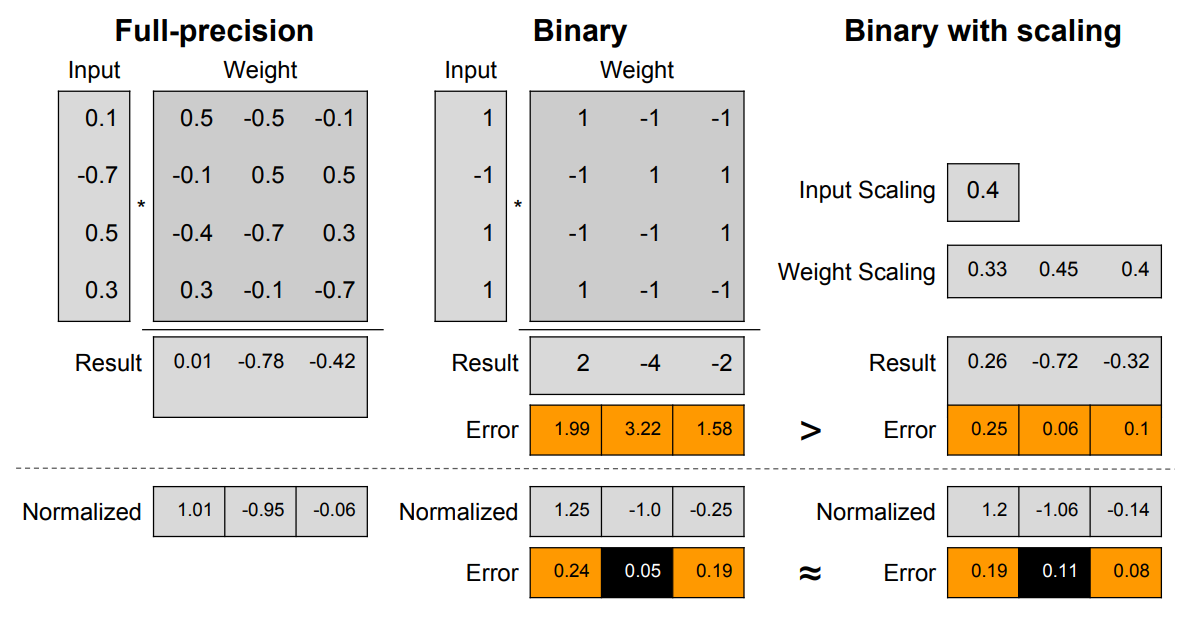
\includegraphics[width=1\textwidth]{Figures/XNOR-Scaling.png}
	\caption{Utilisation de facteurs $\alpha$ et $\beta$ dans une couche denseUtilisation de facteurs $\alpha$ et $\beta$ dans une couche dense}
	\label{fig:XNOR-Dense}
\end{figure}
\FloatBarrier

\subsection{Quantification d'une couche convolutionnelle par produits scalaires }
\begin{remark}
	Nous allons raisonner sur les convolutions à $2$ dimensions. Mais en effet, les résultats peuvent être trivialement généralisés.
\end{remark}
\begin{remark}
	Pour trouver des expressions de $\alpha$ et $\beta,$ nous allons raisonner sur une convolution sans strides ni dilation, ni groupements. On va proposer ensuite un truc qui permet de recouvrer les formules de $\alpha$ et $\beta$ dans ces cas. 
\end{remark}
Soit $\boldsymbol{W}^{(l)}$ une couche convolutionnelle qui prends $C_{\text{in}}$ canaux et donne $C_{\text{out}}$ canaux et dont les noyaux sont de dimensions $(w,h)$.

La formule de $z^{(l)}$ est:
\begin{equation}\label{eq:ConvExpanded}
	\forall c\in\{1,\dots, C_{\text{out}}\},\quad z_c^{(l)}=\sum_{c'=1}^{C_\text{in}} \boldsymbol{W}_{c,c'}^{(l)}*a_{c'}^{(l-1)}
\end{equation}

\begin{remark}
	On peut aussi écrire \eqref{eq:ConvExpanded} sous la forme compacte:
	\begin{equation}
	z^{(l)}= \boldsymbol{W}^{(l)}* a^{(l-1)}
	\end{equation}
	où $\boldsymbol{W}^{(l)}$ est de dimension $C_{\text{out}}\times C_{\text{in}} \times w\times h,$ et $a^{(l-1)}$ est de dimension  $C_\text{in}\times w \times h$
\end{remark}
Pour simplifier, nous allons raisonner sur le cas $C_{\text{out}}=1,$ puis nous allons généraliser:
\subsubsection{Cas d'un seul canal de sortie: $C_{\text{out}}=1$}
On commence par le cas $C_{\text{out}}=1:$
On a:
\begin{align}
	\alpha&=\frac{\left\lVert \boldsymbol{W}^{(l)} \right\rVert_1}{w\cdot h \cdot C_{\text{in}}} \\
	\forall i,j\quad \beta_{i,j}&=\frac{\left\lVert a_{[i,w],[j,h]}^{(l-1)} \right\rVert_1}{w\cdot h \cdot C_{\text{in}} }
\end{align}
avec $a^{(l-1)}_{[i,w],[j,h]}$ est le sous-tenseur de dimensions $C_{\text{in}} \times w \times h$ qui commence à la position $i$ dans son deuxième axe, et $j$ dans son troisième axe.

En faite, $(\beta_{i,j})_{i,j}$ constitue un tenseur $\boldsymbol{\beta}$\footnote{Le temps de calcul de $\boldsymbol{\beta}$ peut être optimisé grâce aux techniques de la programmation dynamique} de dimension $w\times h,$ et la formule de $z^{(l)}$ sera:
\begin{equation} \label{XnorNet:Conv}
	z^{(l)}=\left(\sign \boldsymbol{W}^{(l)} * \sign a^{(l-1)}\right) \odot \boldsymbol{\beta}\alpha
\end{equation}

\subsubsection{Cas général}
Dans le cas où $C_{\text{out}}>1$, on décompose cette couche convolutionnelle en plusieurs convolutions. et on dérive la formule de chacune:
\begin{equation}
	\forall c\in\{1,\dots, C_{\text{out}\}},\quad z_c^{(l)} = \left(\sign \boldsymbol{W}_c^{(l)} * \sign a^{(l-1)}\right) \odot \boldsymbol{\beta}\alpha_c
\end{equation}
Finalement, on peut l'écrire dans la forme compacte:
\begin{equation}
	z^{(l)} = \left(\sign \boldsymbol{W}^{(l)} * \sign a^{(l-1)}\right) \odot \left(\boldsymbol{\alpha} \otimes \boldsymbol{\beta}\right)
\end{equation}
où $\otimes$ est le produit extérieur entre deux tenseurs.

\begin{figure}[h!]
	\centering
	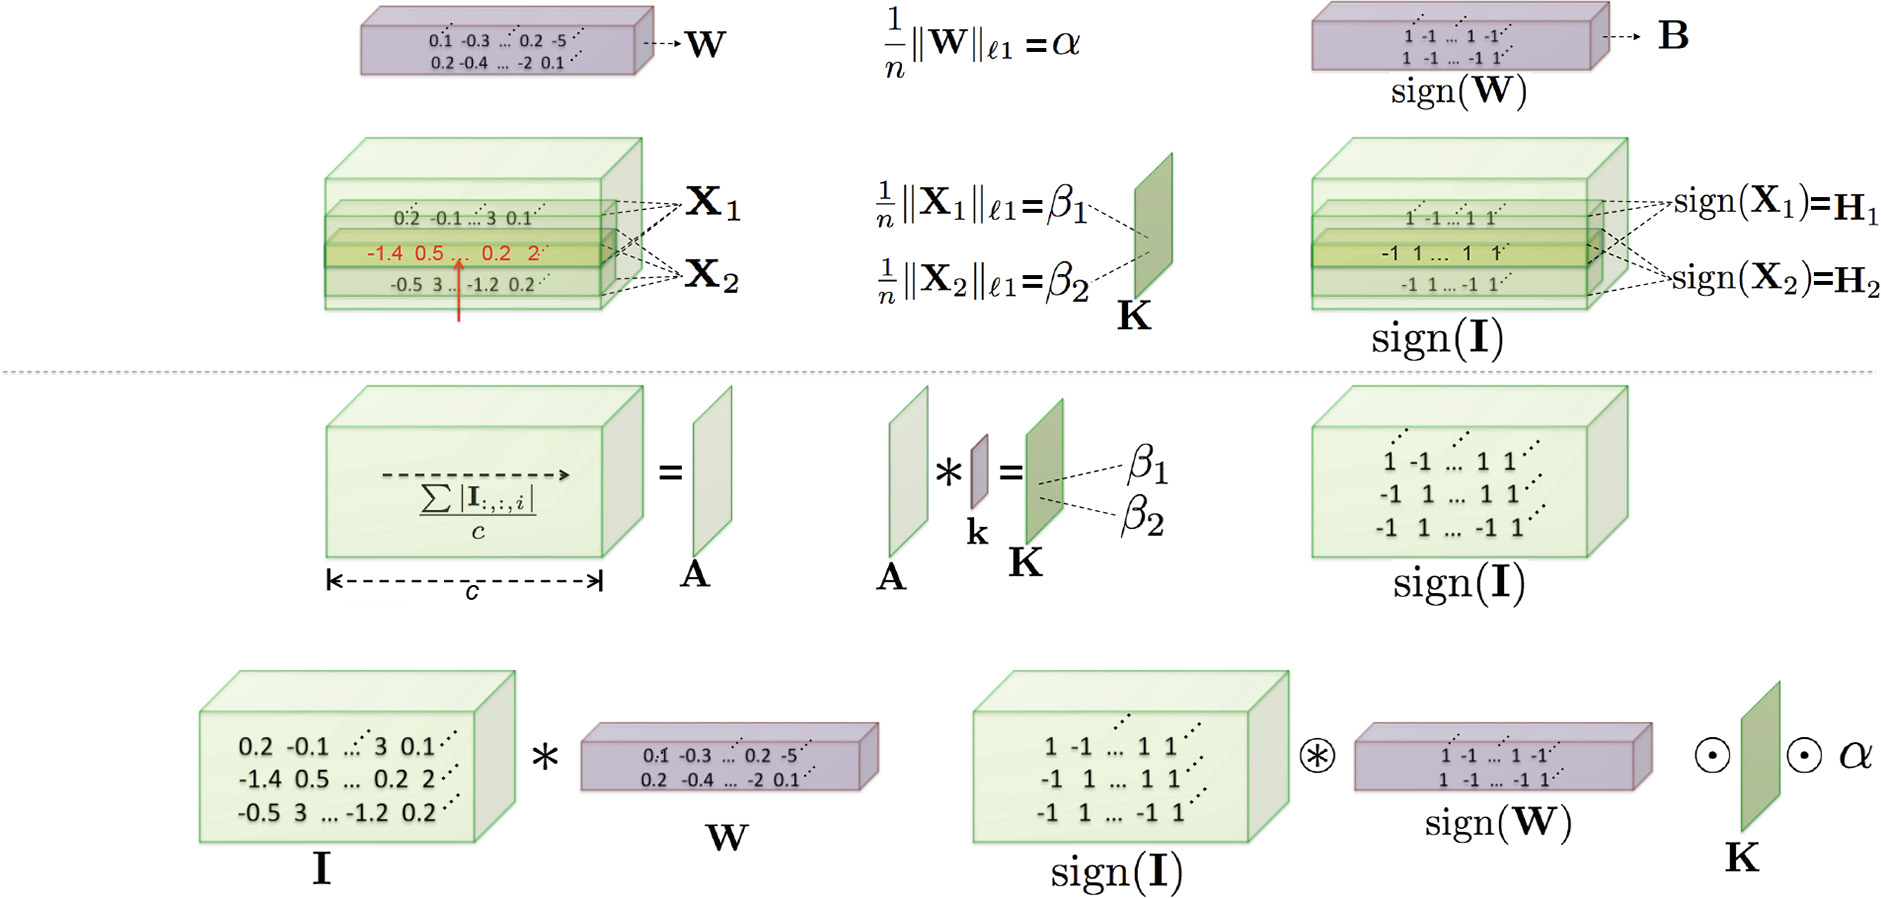
\includegraphics[width=1\textwidth]{Figures/XNOR-Conv2D.png}
	\caption{Utilisation de facteurs $\alpha$ et $\beta$ dans une couche convolutionnelle}
	\label{fig:XNOR-Conv}
\end{figure}
\FloatBarrier
\subsection{Quantification d'une opération bilinéaire quelconque}\label{XnorNet:BilinearForm}
\subsubsection{Hypothèses}
Les hypothèses suivantes ne posent aucune contrainte supplémentaires, en effet on les pose pour formaliser notre démonstration:
\begin{itemize}
\item On suppose que $\boldsymbol{W}^{(l)}$ et $a^{(l-1)}$ sont deux membres des espaces vectoriels réels respectifs $E_l$ et $F_{l-1}.$
\item On suppose que $\star : E_l\times F_{l-1}\rightarrow H_l$ est bilinéaire avec $H_l$ est un espace vectoriel réel de dimension $\dim H_l=s$.
\item On suppose que $\mathcal{B}_1$ et $\mathcal{B}_2$ sont les bases respectifs de  $E_l$ et $F_{l-1}.$
\end{itemize}
\subsubsection{Décomposition de $\star$ en formes bilinéaires}
On a $\star$ peut être décomposé élément par élément en $s$ forme bilinéaire $\star_1,\dots,\star_s:E_l\times F_{l-1} \rightarrow \mathbb{R}.$
\newline Soit $M_i=\mat(\star_i,\mathcal{B}_1,\mathcal{B}_2).$ On a donc:
\begin{equation*}
	\boldsymbol{W}^{(l)}\star a^{(l-1)} = \begin{pmatrix}
	\boldsymbol{W}^{(l)}\star_1 a^{(l-1)}	 \\
	\vdots \\
	\boldsymbol{W}^{(l)}\star_s a^{(l-1)}
		\end{pmatrix} =
	\begin{pmatrix}
		{\boldsymbol{W}^{(l)}}^T M_1 a^{(l-1)}	\\
		\vdots \\
		{\boldsymbol{W}^{(l)}}^T M_s  a^{(l-1)}
	\end{pmatrix} 
\end{equation*}
\subsubsection{Décomposition en valeurs singulières}
Dans cette section, nous allons quantifier chaque forme bilinéaire indépendamment de l'autre.
\newline Soit $i\in\{1,\dots,s\}.$  On a d'après la décomposition en valeurs singulières:
\begin{equation*}
	\exists V_i\in \mathcal{O}(\mathbb{R},m),\exists U_i\in\mathcal{O}(\mathbb{R},n),\exists \Sigma_i\in\mathcal{M}(\mathbb{R},n,m) \ \text{diagonal}\ / \quad \begin{cases}
		M_i= U_i^T \Sigma_i V_i \\ 
		\Sigma_{i,p,p}=\sigma_{i,p} \ge 0 & \forall p\in\{1,\dots,\min(n,m)\} \\
		\Sigma_{i,p,p}=\sigma_{i,p} = 0 & \forall p> \min(n,m)
	\end{cases}
\end{equation*}
On peut encore factoriser $\Sigma_i$ en deux matrices diagonales $A_i\in\mathcal{M}(\mathbb{R},\min(n,m),n)$ et $B_i \in\mathcal{M}(\mathbb{R},\min(n,m),m)$ tels que:
\begin{equation}
	\begin{cases}
	A_{i,p,p}=B_{i,p,p} = \sqrt{\sigma_{i,p}}  &  \forall p \in\{1,\dots,\min(n,m)\} \\
	\Sigma_i = A_i^TB_i
	\end{cases}
\end{equation}
On a donc: 
\begin{align*}
	\boldsymbol{W}^{(l)}\star_i a^{(l-1)} &= {\boldsymbol{W}^{(l)}}^T M_i a^{(l-1)} \\
	&= {\boldsymbol{W}^{(l)}}^T U_i^T A_i^T B_i V a^{(l-1)} \\
	&=\left(A_iU_i \boldsymbol{W}^{(l)}  \right)^T \left(B_i V_i a^{(l-1)}\right) \\
	&= \left\langle A_iU_i \boldsymbol{W}^{(l)}  , B_i V_i a^{(l-1)}  \right\rangle  \addtocounter{equation}{1}\tag{\theequation}
\end{align*}
Pour quantifier ce produit scalaire, on doit d'abord généraliser l'équation \eqref{XnorNet:VectorQuantification:Problem} en:

\begin{equation}\label{XnorNet:TransformedVectorQuantification}
	(\gamma,\tilde{w})=\argmin_{\gamma,\tilde{w}} \lVert A U w -  \gamma A U \tilde{w} \rVert_2^2
\end{equation}
Avec \begin{itemize}
	\item $A\in\mathcal{M}(\mathbb{R},m,n)$ une matrice diagonale dont les coefficient diagonaux $A_{p,p}=\sqrt{\sigma_p}$ sont positifs
	\item $U\in\mathcal{O}(\mathbb{R},n)$ une matrice orthogonale. 
\end{itemize}
\subsubsection{Quantification optimale de $A U w$ }
Avant de résoudre ce problème, nous allons utilisé la propriété suivante:
\begin{equation} \label{SVD:Lemma1}
	U^TA^TA U = A^TA = D ^2
\end{equation}
Avec $D \in\mathcal{M}(\mathbb{R},m)$ la matrice diagonale tels que $D_{p,p}=\sqrt{\sigma_p}$
\newline En effet, en exploitant \eqref{SVD:Lemma1} on a:
\begin{align*}
	\lVert A U w -  \gamma A U \tilde{w} \rVert_2^2 &= \langle A U w,A U w \rangle - 2\gamma \langle A U w, A U \tilde{w} \rangle + \gamma ^2\langle A U \tilde{w},A U \tilde{w} \rangle \\
	&= \langle A U w,A U w \rangle - 2\gamma \langle A U w, A U \tilde{w} \rangle + \gamma ^2\langle A U \tilde{w},A U \tilde{w} \rangle \\
	&= \langle  w,U^TA ^T A U w \rangle - 2\gamma \langle  w, U^TA ^TA U \tilde{w} \rangle + \gamma ^2\langle  \tilde{w},U^TA^T A U \tilde{w} \rangle \\
	&= \langle  w,D^2  w \rangle - 2\gamma \langle  w, D^2 \tilde{w} \rangle + \gamma ^2\langle  \tilde{w},D^2 \tilde{w} \rangle  \\
	&=\langle  D w,D  w \rangle - 2\gamma \langle  D w, D \tilde{w} \rangle + \gamma ^2\langle  D \tilde{w},D \tilde{w} \rangle
\end{align*}
Or on a:
\begin{equation*}
	\langle  D\tilde{w},D \tilde{w} \rangle  = \sum_{i=1}^n \sigma_i \tilde{w}_i^2 = \sum_{i=1}^n \sigma_i
\end{equation*}
Et donc on a:
\begin{equation*}
	\left\lVert \Sigma V w -  \gamma \Sigma V \tilde{w} \right\rVert_2^2 =  \langle  D w,D  w \rangle - 2\gamma \langle  D w, D \tilde{w} \rangle + \gamma ^2\sum_{i=1}^n \sigma_i
\end{equation*}
Maintenant, d'une façon analogue à la démonstration de \ref{XnorNet:VectorQuantification}, on peut montrer que $\langle D w,D \tilde{w} \rangle$ est maximisé pour $\tilde{w} = \sign w$, et donc puisque $\gamma \ge 0,$ on a $	\lVert A U w -  \gamma A U \tilde{w} \rVert_2^2$ est minimisé pour $\tilde{w}=\sign w$ indépendamment de $\gamma.$
\newline En s'inspirant de \ref{XnorNet:VectorQuantification}, on trouve:
\begin{equation} \label{XnorNet:TransformetVectorQuantification:Result}
	\begin{cases}
		\gamma &= \dfrac{\sum_{i=1}^n \sigma_i \lvert w_i \rvert }{\sum_{i=1}^n \sigma_i}\\
		\tilde{w} &= \sign w 
	\end{cases}
\end{equation}
\subsubsection{Quantification optimale de $A_i U_i \boldsymbol{W}^{(l)}$ }
D'après la résolution du problème \eqref{XnorNet:TransformedVectorQuantification}, et en exploitant le résultat \eqref{XnorNet:TransformetVectorQuantification:Result}:
\begin{equation}
	\forall i \in\{1,\dots,r\}	\begin{cases}
		\alpha_i &= \dfrac{\sum_{j=1}^n \sigma_{i,j}\left\lvert \boldsymbol{W}^{(l)}_j \right\rvert }{\sum_{j=1}^n \sigma_{i,j}}\\
		\tilde{\boldsymbol{W}}^{(l)} &= \sign \boldsymbol{W}^{(l)}
	\end{cases}
\end{equation}
\subsubsection{Quantification optimale de $B_i V_i a^{(l-1)}$ }
De même, on trouve que:
\begin{equation}
\forall i \in\{1,\dots,s\}	\begin{cases}
		\beta_i &= \dfrac{\sum_{j=1}^n \sigma_{i,j} \left\lvert a^{(l-1)}_j \right\rvert }{\sum_{j=1}^n \sigma_{i,j}}\\
		\tilde{a}^{(l-1)} &= \sign a^{(l-1)}
	\end{cases}
\end{equation}

\subsubsection{Quantification de l'opérateur bilinéaire}
Le résultat final est peut être écrit sous cette forme compacte:
\begin{equation}\label{XnorNet:BilnearForm:Result}
	\boldsymbol{W}^{(l)}\star a^{(l-1)} \approx  \left( \sign \boldsymbol{W}^{(l)} \star \sign a^{(l-1)}\right) \odot \boldsymbol{\alpha} \odot \boldsymbol{\beta}
\end{equation}

\pagebreak
\section{ABCNet}
\subsection{Conception}
ABCNet\cite{ABCNetPaper} est un réseau de neurones binaires basé sur XNOR-Net, son nom est une abbréviation de "Accurate Binary Convolutional Network", et donc comme son nom suggeste, il est très performant (comparable à un CNN classique). 
\newline Il peut être considéré comme une amélioration directe de XnorNet, puisqu'il réduit l'erreur de quantification d'une variable en faisant une somme pondérée de binarisations prédéfinie.
\begin{figure}[h!]
	\centering
	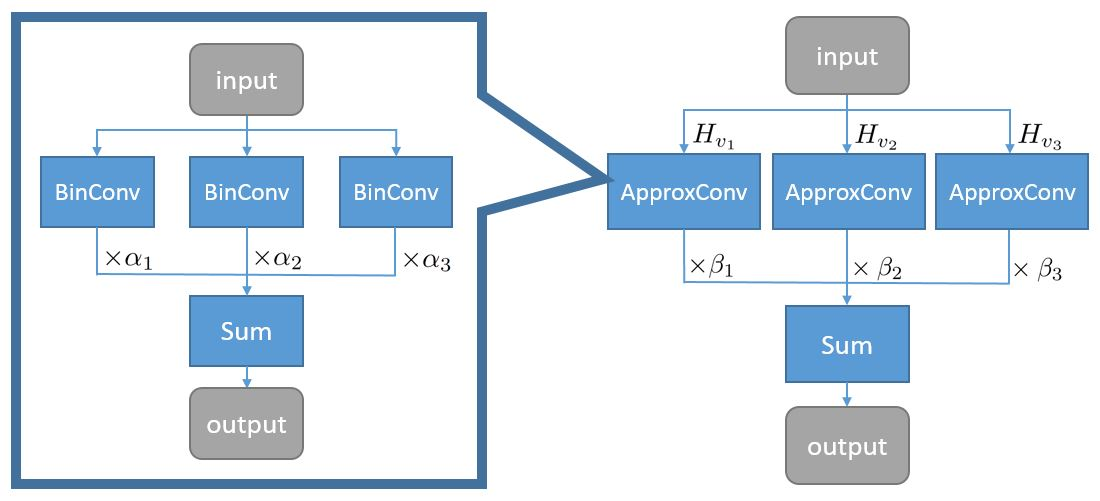
\includegraphics[width=\textwidth]{Figures/ABCNet.png}
	\caption{Exemple d'un ABCNet à une seule couche}
	\label{fig:ABCNet}
\end{figure}
\subsection{Toplogie}
Le ABCNet\cite{ABCNetPaper} est conçu explicitement pour les réseaux de neurones binaires convolutionnelles. 

Mais comme le XNOR-NET, il peut être généralisé à n'importe quel architecture (dense, récurrente, etc...)
\subsection{Objectif}
\subsubsection{Notations}
On dénote par
\begin{enumerate}
	\item $\Psi_1,\dots,\Psi_n$ des binarisations de  $\boldsymbol{W}^{(l)}$
	\item $\Phi_1,\dots,\Phi_m$ des binarisations de  $a^{(l-1)}$
\end{enumerate}
\subsubsection{Approximation par combinaisons linéaires}
L'objectif d'un ABCNet est d'approximer $\boldsymbol{W}^{(l)}$ en une combinaison linéaires de $n$ binarisations, et $a^{(l-1)}$ en $m$ une combinaison linéaires de $m$ binarisations.

On veut trouver $\left(\Psi_1,\dots,\Psi_n\right), \left(\Phi_1,\dots,\Phi_m\right),(\alpha_1,\dots,\alpha_n)\in\mathbb{R}_+^n,(\beta_1,\dots,\beta_m)\in\mathbb{R}_+^m $ tel que:
\begin{align}
	\boldsymbol{W}^{(l)}&\approx \sum_{i=1}^n \alpha_i \Psi_i(\boldsymbol{W}^{(l)}) \label{ABCNet:W}  \\
	a^{(l-1)}&\approx \sum_{i=1}^m \beta_i \Phi_i(a^{(l-1)}) \label{ABCNet:a}\\
	\boldsymbol{W}^{(l)} \star a^{(l-1)} &\approx \sum_{i=1}^n\sum_{j=1}^m  \alpha_i  \beta_j\Psi_i(\boldsymbol{W}^{(l)})\star  \Phi_j(a^{(l-1)}) \label{ABCNet:z}
\end{align}

\subsection{Choix de binarisations de $\boldsymbol{W}^{(l)}$}
Il y'a plusieurs méthodes pour choisir les binarisations de $\boldsymbol{W}^{(l)}$
\subsubsection{Base orthogonale de Hadamard}
Cette technique crée des binarisations qui ne dépendent pas de $\boldsymbol{W}^{(l)}.$ En interprétant $\boldsymbol{W}^{(l)}$ comme un vecteur d'un espace euclidien $E$ de dimension $r=2^s\ge n.$ On  cherche la matrice de Hadamard $H_s,$ puis on choisit $n$ colonnes (ou lignes) $\Psi_1,\dots,\Psi_n$.

Dans ce cas, la famille $(\Psi_1,\dots,\Psi_n)$ induit un sous-espace $F$ de $E$ de dimension $n.$  
\newline Ainsi, le problème est réduit à une projection orthogonale de $E$ vers $F$    
\newline En notant $K=\mat(\Psi_1,\dots,\Psi_n),$ la valeur optimale de $\boldsymbol{\alpha}$ qui minimise l'erreur quadratique de quantification est:
\begin{equation}
	\boldsymbol{\alpha} = K^T\boldsymbol{W}^{(l)}
\end{equation}

\subsubsection{Famille de fonctions $\sign$ décalées } 
Cette technique crée des binarisations de la forme:
\begin{equation}
	\Psi_i\left(\boldsymbol{W}^{(l)}\right) = \sign \left( \boldsymbol{W}^{(l)} +\mu_i\right) 
\end{equation}
Avec $\mu_1,\dots,\mu_n\in\mathbb{R}$ un paramètre de décalage. Il peut être entraînable ou non.

\subsubsection{Approximation par distribution}
Cette technique se base sur l'observation que la distribution des poids (non-binarisés) est dense\cite{ABCNetPaper}, et elle est proche d'une distribution normale. L'expression de $\Psi_i$ est:
\begin{equation}
	\Psi_i\left(\boldsymbol{W}^{(l)}\right)=\sign\left( \boldsymbol{W}^{(l)}-\mathbb{E}\left[ \boldsymbol{W}^{(l)} \right] + \mu_i \sqrt{\mathbb{V}\left[ \boldsymbol{W}^{(l)} \right]}\right)
\end{equation}
Où \begin{itemize}
	\item $\mathbb{E}\left[ \boldsymbol{W}^{(l)} \right]$ est un estimateur de l'espérence de la distribution des paramètres: c'est la valeur moyenne de tous ces paramètres.
	\item  $\mathbb{V}\left[ \boldsymbol{W}^{(l)} \right]$ est une estimation de leur variance.
	\item $\mu_i$ est fixe ou entraînable.
\end{itemize}
Quelque soit le cas, on peut initialiser $\mu_i$\cite{ABCNetPaper} par:
\begin{equation}
	\mu_i=-1+2\cdot \frac{i-1}{n-1}
\end{equation}

\subsection{Choix de binarisations de $a^{(l)}$}
Puisque $a^{(l)}$ dépend toujours de l'entrée $x.$ Pour cela $a^{(l)}$ va généralement varier d'une inférence à une autre.
\newline Pour cela, on doit créer des binarisations qui dépendent de $a^{(l)}.$ Par exemple, on peut choisir:
\subsubsection{Famille de fonctions $\sign$ décalées}
Cette technique crée des binarisations de la forme:
\begin{equation}
	\Psi_j\left(a^{(l)}\right) = \sign \left( a^{(l)} +\kappa_j\right) 
\end{equation}
Avec $\kappa_1,\dots,\kappa_m\in\mathbb{R}$ un paramètre de décalage. Il peut être entraînable ou non.

\subsubsection{Approximation par distribution}
\begin{equation}
	\Phi_j\left(a^{(l)}\right)=\sign\left( a^{(l)}-\mathbb{E}\left[a^{(l)} \right] + \kappa_j \sqrt{\mathbb{V}\left[ a^{(l)} \right]}\right)
\end{equation}
Où \begin{itemize}
	\item $\mathbb{E}\left[ a^{(l)} \right]$ est une estimation de l'espérence de $a^{(l)}$ dans le lot courant.
	\item  $\mathbb{V}\left[a^{(l)} \right]$ est une estimation de la variance de $a^{(l)}$ dans le lot courant
	\item $\kappa_j$ est fixe ou entraînable.
\end{itemize}

Dans la phase d'inférence, pour éviter le côut de calcul des paramètres statistiques, on peut remplacer:
\begin{itemize}
	\item $\mathbb{E}\left[ a^{(l)} \right]$ du lot courant par $K_1=\mathbb{E}_B\left[\mathbb{E}\left[ a^{(l)} \right]\right],$ qui est la valeur moyenne de tous les lots du jeu de données.
	\item $\mathbb{V}\left[ a^{(l)} \right]$ du lot courant par $K_2=\frac{m}{m-1}\mathbb{E}_B\left[\mathbb{V}\left[a^{(l)} \right]\right]$, qui est une estimation sans bias de la variance de $a^{(l)}$ dans tous les lots du jeu de données, avec $m$ la taille de lot.
\end{itemize}

\subsection{Quantification par tenseur binaire}
C'est la méthode ou on fait les quantifications de $\boldsymbol{W}^{(l)}$ et $a^{(l-1)}$ en suivant les équations respectifs \eqref{ABCNet:W} et \eqref{ABCNet:a}
\newline La quantification de $z^{(l)}$ va respecter l'équation $\eqref{ABCNet:z}.$

\subsection{Quantification par produit scalaire}
La quantification par produit scalaire est une variante dans laquelle les variables $\alpha_1,\dots,\alpha_n$ de \eqref{ABCNet:W} et $\beta_1,\dots,\beta_m$ de \eqref{ABCNet:a} sont calculéss pour chaque produit scalaire.
\newline C'est à dire, L'équation $\eqref{ABCNet:z}$ est décomposée terme par terme en des produits scalaires, dans chacune on cherche les $(\alpha_i)_{i\in\{1,\dots,j\}}$ et $(\beta_j)_{j\in\{1,\dots,m\}}.$
\subsubsection{Couche Dense}
C'est une généralisation de l'équation \eqref{XnorNet:FullyConnected} de XnorNet.
\newline On a:
\begin{align*}
	\boldsymbol{W}^{(l)}\cdot a^{(l-1)} &\approx  \begin{pmatrix}
		 \left\langle \sum_{i=1}^n \alpha_{i,1}\Psi_i \left(\boldsymbol{W}_1^{(l)}\right),\sum_{j=1}^m \beta_j\Phi_j \left( a^{(l-1)}\right) \right\rangle  \\
		\vdots  \\
		\left\langle \sum_{i=1}^n \alpha_{i,n_l}\Psi_i \left(\boldsymbol{W}_{n_l}^{(l)}\right),\sum_{j=1}^m  \beta_j\Phi_j\left( a^{(l-1)}\right) \right\rangle 
	\end{pmatrix} \\
	&\approx  \begin{pmatrix}
		 \sum_{i=1}^n \sum_{j=1}^m \left \langle \alpha_{i,1}  \Psi_i \left(\boldsymbol{W}_1^{(l)}\right), \beta_j \Phi_j \left( a^{(l-1)}\right) \right\rangle  \\
		\vdots  \\
		\sum_{i=1}^n \sum_{j=1}^m \left \langle \alpha_{i,n_l}  \Psi_i \left(\boldsymbol{W}_{n_l}^{(l)}\right), \beta_j \Phi_j \left( a^{(l-1)}\right) \right\rangle 
	\end{pmatrix} \\
	&\approx   \sum_{i=1}^n \sum_{j=1}^m  \begin{pmatrix}
		\left \langle \alpha_{i,1}  \Psi_i \left(\boldsymbol{W}_1^{(l)}\right), \beta_j \Phi_j \left( a^{(l-1)}\right) \right\rangle  \\
		\vdots  \\
		\left \langle \alpha_{i,n_l}  \Psi_i \left(\boldsymbol{W}_{n_l}^{(l)}\right), \beta_j \Phi_j \left( a^{(l-1)}\right) \right\rangle 
	\end{pmatrix} \\
	&\approx \sum_{i=1}^n\sum_{j=1}^m \beta_j  \left(\Psi_i \left(\boldsymbol{W}^{(l)}\right) \cdot \Phi_j\left(\sign a^{(l-1)}\right)\right) \odot \boldsymbol{\alpha}_i \addtocounter{equation}{1}\tag{\theequation} \label{ABCNet:FullyConnected}
\end{align*}
\subsubsection{Couche convolutionnelle}
C'est une généralisation de l'équation \eqref{XnorNet:Conv} de XnorNet\cite{XnorNetPaper}.
\newline On a:
\begin{equation} \label{ABCNet:Conv}
	\boldsymbol{W}^{(l)}a^{(l-1)} \approx \sum_{i=1}^n\sum_{j=1}^m\left(\Psi_i\left( \boldsymbol{W}^{(l)}\right) * \Phi_j\left( a^{(l-1)}\right)\right) \odot \left(\boldsymbol{\alpha}_i \otimes \boldsymbol{\beta}_j\right) 
\end{equation}
\subsubsection{Opérateur bilinéaire quelconque}\label{ABCNet:BilinearForm}
C'est une généralisation de \ref{XnorNet:BilinearForm}, l'équation \eqref{XnorNet:BilnearForm:Result} va être généralisé en:
\begin{equation}\label{ABCNet:BilnearForm:Result}
	\boldsymbol{W}^{(l)}\star a^{(l-1)} \approx \sum_{i=1}^n\sum_{j=1}^m  \left( \Psi_i\left(\boldsymbol{W}^{(l)}\right) \star \Phi_j \left(a^{(l-1)}\right)\right) \odot \boldsymbol{\alpha}_i \odot \boldsymbol{\beta}_j
\end{equation}
\newpage 
\section{BiRealNet}
\subsection{Conception}
BiRealNet\cite{BiRealNetPaper} est un réseau de neurones binarisés basés sur BinaryNet.
\newline Son nom signifie le faite que s'il est binaire, il a aussi le comportement continu présent dans les réseaux de neurones classiques à valeurs réelles.
\newline Il n'est pas basé sur la quantification comme les autres BNNs, mais sur l'architecture du réseau. En effet il réduit la perte d'information causé par la quantification par l'ajout des connexions résiduelles. Dans BiRealNet les connexions résiduales sont sous la forme d'une somme simple.
\begin{figure}[h!]
	\centering
	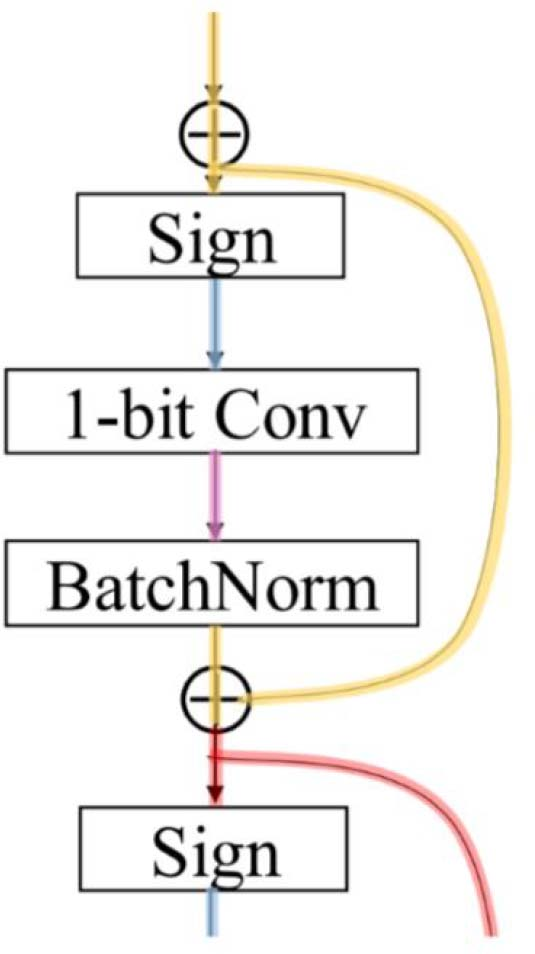
\includegraphics[width=0.25\textwidth]{Figures/BiRealNet.png}
	\caption{Exemple d'une liaison résiduale d'un BiRealNet}
	\label{fig:BiRealNet}
\end{figure}

\subsection{Topologie}
BiRealNet\cite{BiRealNetPaper} est pratiquement indépendent de la topologie elle même. Mais la présence des liaisons résiduales y induit quelques contraintes.
\newline La principale contrainte que la couche résiduale et la couche actuelle doivent avoir les même dimensions.

\subsection{Block BiRealNet}
Pour bien augmenter l'apport d'informations avec BiRealNet, la connexion résiduale est faite entre deux blocs connexes et qui vérifient la contrainte sur les dimensions.
\newline De plus, le résidu doit avoir la possibilité de varier sur un ensemble réel. C'est à dire varier sur un grands ensemble de valeurs.
\newline Un exemple concis est la figure \ref{fig:BiRealNet} qui montre une connexion résiduale pour chaque bloc de:
\begin{itemize}
	\item Quantification par signe
	\item Convolution binarisée
	\item Normalisation par Lots
\end{itemize}
En effet, selon cette figure, la connexion va être faite entre le résultat du bloc actuel et le bloc précédent.
\subsection{Liaison résiduale}
\subsubsection{Notation}
Soit $\mathcal{R}(l)$ l'ensemble de couches qui ont une liaison résiduale avec la $l^\text{ème}$ couche.
\subsubsection{Contraintes sur $\mathcal{R}(l)$}
Dans BiRealNet, la seule contrainte présente est que le réseau de neurone doit rester acyclique:
\begin{equation}
	\forall l,\forall l' \in \mathcal{R}(l), \quad l' < l
\end{equation}
\subsubsection{Equation}
La liaison résiduale induit un changement de la formule de $z^{(l)}$ trouvée dans le tableau \ref{table:AcyclicNeuralNetwork} situé dans la section \ref{Theoretical:Observations}. La nouvelle expression de $z^{(l)}$ est:
\begin{equation}\label{BiRealNet:Expression}
	z^{(l)}=\boldsymbol{W}^{(l)}\tilde{\star} a^{(l-1)}+\sum_{l' \in \mathcal{R}(l)}z^{(l')}
\end{equation}

Dans cette équation, $\tilde{\star}$ signifie que l'opérateur $\star$ est quantifié avec une quantification quelconque.
Dans la plus part des cas, $\mathcal{R}(l)$ est un singleton qui contient seulement la couche du dernier bloc, ce qui est le cas par exemple pour la figure \ref{fig:BiRealNet}

\subsection{Choix de la quantification}
Dans l'équation \eqref{BiRealNet:Expression}, nous n'avons explicité aucune quantification, et c'est l'une des avantages de BiRealNet: il est orthogonal au type de binarisation\footnote{En effet, BiRealNet est un modèle basé sur l'architecture, et ces modèles sont généralement orthogonaux aux modèles basées sur la quantification, dans le sens ou en peut créer un modèle en exploitant en même temps une quantification d'un et une architecture de l'autre.}.
\newline Ainsi, l'opérateur quantifié $\tilde{\star}$ peut être basé sur BinaryNet, XnorNet, ABCNet, etc...
\chapter{Implémentation}

\section{Introduction}

Dans ce chapitre, on va implémenter les modèles qu'on a décri dans le chapitre précédent tout en suivant les paradigme que Keras et Larq respectent.
\paragraph{Définition des types}
Bien que Python est dynamiquement typé, nous allons inférer dans ce chapitre et dans notre bibliothèque un typage statique pour faciliter la compréhension.
\newline Nous allons dénoter pour un ensemble de types $T,T_1,\dots,T_n,Q,Q_1,\dots,Q_m$:
\begin{itemize}
	\item $\texttt{List}[T]$ pour n'importe quel itérable sur $T$
	\item $\texttt{Tuple}[T_1,\dots,T_n]$ pour un tuple contenant  des éléments de $T_1,\dots,T_n$ dans l'ordre indiqué.
	\item $\mathcal{T}[T]=\texttt{Tensor}[T]$  pour un type compatible avec 	\texttt{tensorflow.Tensor} avec \texttt{dtype}=$T$
	\item $\mathcal{T}[T,n]=\texttt{Tensor}[T,n]$  pour un type compatible avec 	\texttt{tensorflow.Tensor} avec un rang égal à $n$ et avec \texttt{dtype}=$T$
	\item $\mathcal{V}[T]=\texttt{Vector}[T]$ pour un type compatible avec 	\texttt{tensorflow.Tensor} avec un rang égal à $1$ et avec \texttt{dtype}=$T$
	\item $\mathcal{M}[T]=\texttt{Matrix}[T]$  pour un type compatible avec 	\texttt{tensorflow.Tensor} avec un rang égal à $2$ et avec \texttt{dtype}=$T$
	\item $\mathcal{R}[T]=\texttt{Random}[T]$ pour une fonction aléatoire sans arguments.
	\item $\mathcal{F}[T_1,\dots,T_n\rightarrow Q_1,\dots,Q_m]=\texttt{Function}[T_1,\dots,T_n\rightarrow Q_1,\dots,Q_m]$ pour une fonction dont les arguments sont de types respectifs $T_1,\dots,T_n$ et dont les valeurs sonts de types respectifs $Q_1,\dots,Q_m$
	\item $\End[T]=\texttt{Function}[T_1,\dots,T_n\rightarrow T_1,\dots,T_n]$ pour une fonction dont l'argument et les valeurs sont de types respectifs $T_1,\dots,T_n$. 
	\item $\mathcal{P}[T_1,\dots,T_n]=\texttt{Predicate}[T_1,\dots,T_n]$ pour un prédicat (fonction booléenne)  acceptant $n$ arguments de types respectifs $T_1,\dots,T_n$
\end{itemize}
\newpage
\section{Paradigmes}
\subsection{Dans l'implémentation de BinaryFlow}\label{Paradigm:Implementation}
Dans l'implémentations de la bibliothèque BinaryFlow, nous avons adopté principalement:
\begin{itemize}
	\item La programmation orientée objet
	\item La programmation générique
\end{itemize}
\subsubsection{Programmation orientée objet}

\subsubsection{Programmation générique}

\subsection{Dans l'utilisation de BinaryFlow}\label{Paradigm:User}
Etant une extension de Keras et Larq, nous recommenderions l'utilisateur à suivre les bonnes pratiques de ces bibliothèques.
\newline En effet nous encouragerions à suivre une de ces interfaces:
\begin{itemize}
	\item L'interface Séquentielle
	\item L'interface fonctionnelle
	\item L'interface orientée objet
\end{itemize}
\subsubsection{Interface séquentielle}
C'est l'interface la plus facile à exploiter, mais naturellement elle ne supporte pas les couches résiduales.
\newline L'utilisation de cette interface sert à créer une objet de type \texttt{tensorflow.keras.Sequential} contenant la séquence des couches dont le type est \texttt{List[tensorflow.keras.layers.Layer]}


\subsubsection{Interface fonctionnelle}
Cette interface met en valeur le fait qu'un modèle se traduit en des fonctions évaluer dans un certian ordre à un tenseur initial $X$.
\newline Pour cela, cette interface introduit un tenseur symbolique $\boldsymbol{X}$ qui décrit l'entrée du réseau de neurones. Puis les fonctions sont appliqués au tenseur $\boldsymbol{X}$ pour établir le modèle et fixer les dimensions de:
\begin{itemize}
	\item Ces paramètres
	\item L'entrée de chaque fonction
	\item La sortie de chaque fonction
\end{itemize}
Une fois le modèle est construit, on peut l'entraîner, et puis le déployer.

\subsubsection{Interface orientée objet}
Cette interface met en valeur l'aspect orienté objet de TensorFlow (et aussi BinaryFlow), il se base sur le faite qu'un utilisateur peut définir son modèle en héritant de la classe \texttt{tensorflow.keras.Model}
\newline En utilisant cette interface, l'utilisateur peut surcharger les méthodes de \texttt{tensorflow.keras.Model}, ce qui lui permet de personnaliser:
\begin{itemize}
	\item L'entraînement du modèle
	\item L'inférence du modèle
	\item L'évaluation du modèle
	\item La fonction coût du modèle
	\item ...
\end{itemize}

\subsubsection{Interface bas niveaux}
Cette interface utilise directement les fonctionnalités de TensorFlow sans exploiter Keras. Elle est aussi supportée par BinaryFlow, mais on ne la recommende que pour les utilisateurs avancés.

\subsection{Dans l'extension de BinaryFlow}
Pour éténdre notre bibliothèques, nous recommenderions de suivre les paradigmes utilisées dans l'implémentation qui sont décrite dans la section \ref{Paradigm:Implementation}.

\section{Conception}
BinaryFlow est implémentés sous formes des modules suivants:
\begin{itemize}
	\item Module des couches
	\item Module des blocs
	\item Module des quantificateurs
	\item Module des coûts
\end{itemize}

\begin{figure}[htp]
	\centering
	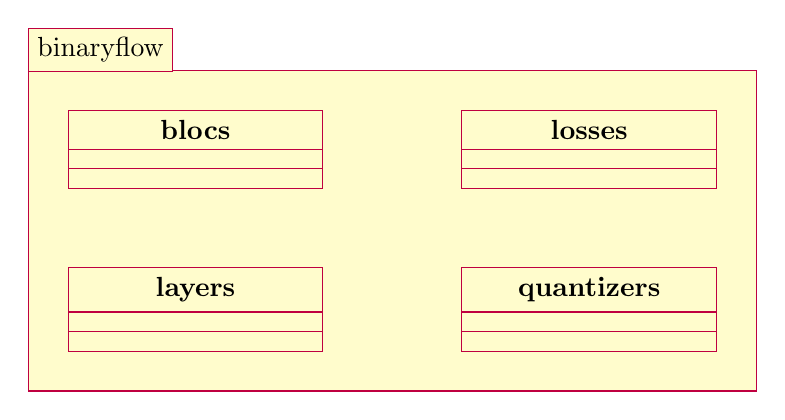
\begin{tikzpicture}
	\begin {package}{binaryflow}
		\begin {class}[text width=3cm]{layers}{0 ,0}
		\end{class}
		\begin {class}[text width=3cm]{blocs}{0 ,2cm}
		\end{class}
		\begin {class}[text width=3cm]{quantizers}{5cm ,0}
		\end{class}
		\begin {class}[text width=3cm]{losses}{5cm ,2cm}
		\end{class}
	\end{package}
	\end{tikzpicture}
	\caption{Structure de la bibliothèque}
\end{figure}


Dans les sections suivantes nous allons parler de chaque module.
\section{Couches}
Ce module est l'implémentation des couches des modèles suivant:
\begin{itemize}
	\item BinaryNet
	\item XnorNet
	\item ABCNet
\end{itemize}
Dans ce module, chaque couche admet un nom de la forme \texttt{NomModèle.TypeCouche} avec:
\begin{itemize}
	\item $\texttt{NomModèle} \in \{\texttt{BinaryNet},\texttt{XnorNet},\texttt{ABCNet}\}$
	\item $\texttt{TypeCouche} \in \{\texttt{Dense},\texttt{Conv1D},\texttt{Conv2D},\texttt{Conv3D}\}$
\end{itemize} 

\begin{figure}[htp]
	\small
	\centering
	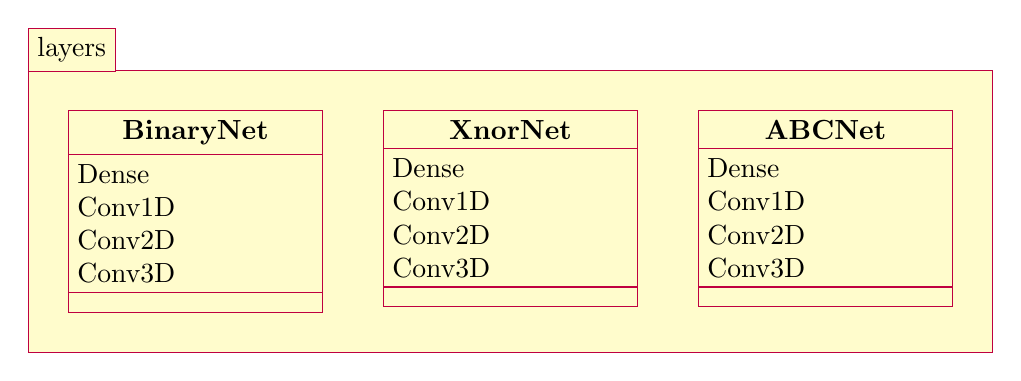
\begin{tikzpicture}
		\begin {package}{layers}
			\begin {class}[text width= 3cm]{BinaryNet}{0, 0}
			\attribute{Dense}
			\attribute{Conv1D}
			\attribute{Conv2D}
			\attribute{Conv3D}
			\end{class}
			\begin {class}[text width= 3cm]{XnorNet}{4cm ,0cm}
						\attribute{Dense}
			\attribute{Conv1D}
			\attribute{Conv2D}
			\attribute{Conv3D}
			\end{class}
			\begin {class}[text width= 3cm]{ABCNet}{8cm ,0cm}
						\attribute{Dense}
			\attribute{Conv1D}
			\attribute{Conv2D}
			\attribute{Conv3D}
			\end{class}
		\end{package}
	\end{tikzpicture}
	\caption{Le contenu de \texttt{layers}}
\end{figure}
\FloatBarrier
\newpage
\subsection{BinaryNet}\label{BinaryNet:Module}
Le module \texttt{BinaryNet} contient $4$ classes qui sont: \texttt{Dense},\texttt{Conv1D},\texttt{Conv2D} et \texttt{Conv3D}.
Nous avons définir ces classes comme des synonymes respectivement de \texttt{Larq.layers.QuantDense},\texttt{Larq.layers.QuantConv1D},\texttt{Larq.layers.QuantConv2D} et \texttt{Larq.layers.QuantConv3D}
\subsubsection{API commun}
Ces $4$ couches admettent des attributs similaires, qui sont:
\begin{itemize}
	\item \texttt{kernel\_quantizer} qui est la quantification de poids.
	\item \texttt{input\_quantizer} qui est la quantification des noeuds. 
	\item \texttt{kernel\_constraint} qui est la contrainte sur les poids.
\end{itemize}
Pour conformer à la formulation originale de BinaryNet \cite{BinaryNetPaper} et BinaryConnect \cite{BinaryConnectPaper} ces valeurs doivent être initialisés à 

\begin{table}[ht]
	\centering
	\begin{tabularx}{\textwidth}{| p{3.5cm} | X |}
		\hline
		Attribut & Valeur \\
		\hline
		 \texttt{kernel\_quantizer} & \begin{itemize}
		 	\item \texttt{Larq.quantizers.SteSign}
		 	\item \texttt{BinaryFlow.quantizers.StochasticSteSign}
		 \end{itemize}  \\ 
		\hline
		\texttt{input\_quantizer} & \begin{itemize}
			\item \texttt{Larq.quantizers.SteSign}
			\item \texttt{BinaryFlow.quantizers.StochasticSteSign}
		\end{itemize}  \\ 
		\hline 
		\texttt{kernel\_constraint} & \begin{itemize}
			\item \texttt{weight\_clip}
		\end{itemize}  \\ 
		\hline
	\end{tabularx}
	\caption{Terminologie de la division en Lots}
	\label{table:BinaryNetInitialisation}
\end{table}
\FloatBarrier
\subsubsection{Dense}
Les attributs définissant cette couches sont:
\begin{itemize}
	\item \texttt{units} qui est la dimension de sortie
	\item \texttt{kernel} qui est la matrice de paramètres
\end{itemize}
\subsubsection{ConvND}
Les couches convolutionnelles admettent des attributs similaires.
\newline Pour une couche convolutionnelle à $N\in\{1,2,3\}$ dimensions, on a:
\begin{itemize}
	\item \texttt{filters} est le nombre de canaux de sorties.
	\item \texttt{kernel\_size} est la taille du noyau de convolution
	\item \texttt{padding} est le padding utilisée dans la convolution.
	\item \texttt{strides} est la taille de pas entre deux convolutions successives
\end{itemize} 
\begin{figure}[htp]
	\small
	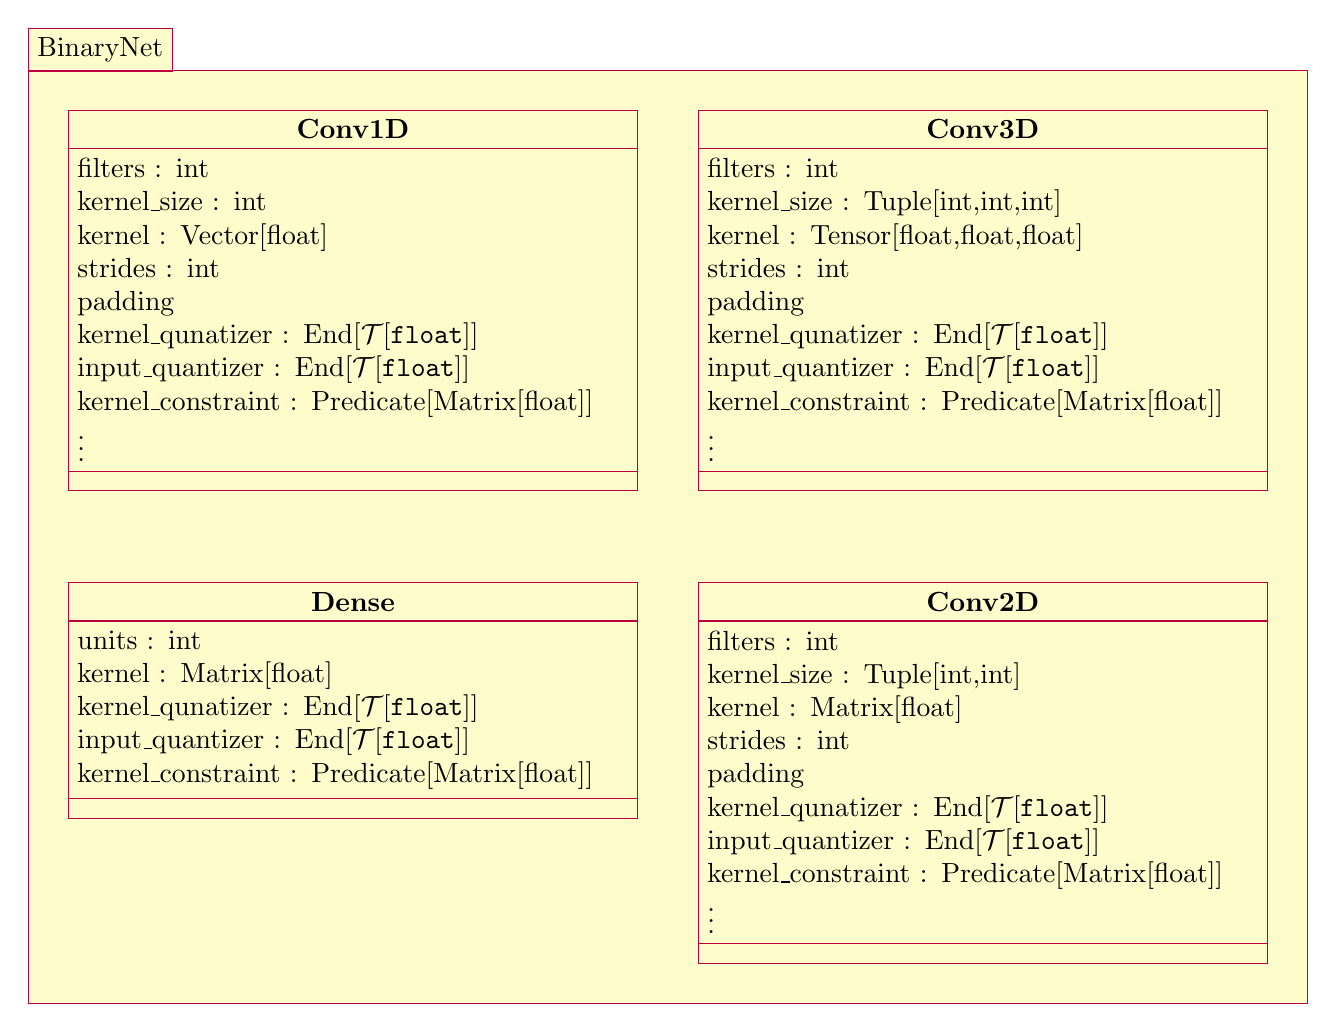
\begin{tikzpicture}
		\begin {package}{BinaryNet}
		\begin {class}[text width= 7cm ]{Dense}{0, 0}
		\attribute{units : int}
		\attribute{kernel : Matrix[float]}
		\attribute{kernel\_qunatizer : $\End[\mathcal{T}[\texttt{float}]]$}
		\attribute{input\_quantizer : $\End[\mathcal{T}[\texttt{float}]]$}
		\attribute{kernel\_constraint : Predicate[Matrix[float]]}
		\vdots
	\end{class}
	\begin {class}[text width= 7cm ]{Conv1D}{0 ,6cm}
	\attribute{filters : int}
	\attribute{kernel\_size : int}
	\attribute{kernel : Vector[float]}
	\attribute{strides : int}
	\attribute{padding}
	\attribute{kernel\_qunatizer : $\End[\mathcal{T}[\texttt{float}]]$}
	\attribute{input\_quantizer : $\End[\mathcal{T}[\texttt{float}]]$}
	\attribute{kernel\_constraint : Predicate[Matrix[float]]}
	\attribute{\vdots}
	\end{class}
	\begin {class}[text width= 7cm ]{Conv2D}{8cm ,0}
	\attribute{filters : int}
	\attribute{kernel\_size : Tuple[int,int]}
	\attribute{kernel : Matrix[float]}
	\attribute{strides : int}
	\attribute{padding}
	\attribute{kernel\_qunatizer : $\End[\mathcal{T}[\texttt{float}]]$}
	\attribute{input\_quantizer : $\End[\mathcal{T}[\texttt{float}]]$}
	\attribute{kernel\_constraint : Predicate[Matrix[float]]}
	\attribute{\vdots}
	\end{class}
	\begin {class}[text width= 7cm ]{Conv3D}{8cm ,6cm}
	\attribute{filters : int}
	\attribute{kernel\_size : Tuple[int,int,int]}
	\attribute{kernel : Tensor[float,float,float]}
	\attribute{strides : int}
	\attribute{padding}
	\attribute{kernel\_qunatizer : $\End[\mathcal{T}[\texttt{float}]]$}
	\attribute{input\_quantizer : $\End[\mathcal{T}[\texttt{float}]]$}
	\attribute{kernel\_constraint : Predicate[Matrix[float]]}
	\attribute{\vdots}
	\end{class}
	\end{package}
\end{tikzpicture}
\caption{BinaryNet}
\end{figure}
\FloatBarrier
\newpage 
\subsection{XnorNet}
Le module \texttt{XnorNet} contient $4$ classes qui sont: \texttt{Dense},\texttt{Conv1D},\texttt{Conv2D} et \texttt{Conv3D}.
\newline Chacune de ces classes est une classe fille de son contrepart dans le module \texttt{BinaryNet} présenté dans \ref{BinaryNet:Module}. 
\subsubsection{Attributs Ajouté}
Le seul attribut ajouté est \texttt{alpha\_trainable} qui demande si $\alpha$ doit être entrainé ou non. Par défaut il est égal à \texttt{False}.
\subsubsection{Initialisaiton de $\alpha$}
Indépendemment de \texttt{alpha\_trainable}, $\alpha$ est toujours initialisé à \ref{XnorNet:FullyConnected} dans le cas d'une couche dense, et à \ref{XnorNet:FullyConnected} dans le cas d'une couche convolutionnelle.
\begin{figure}[htp]
	\small
	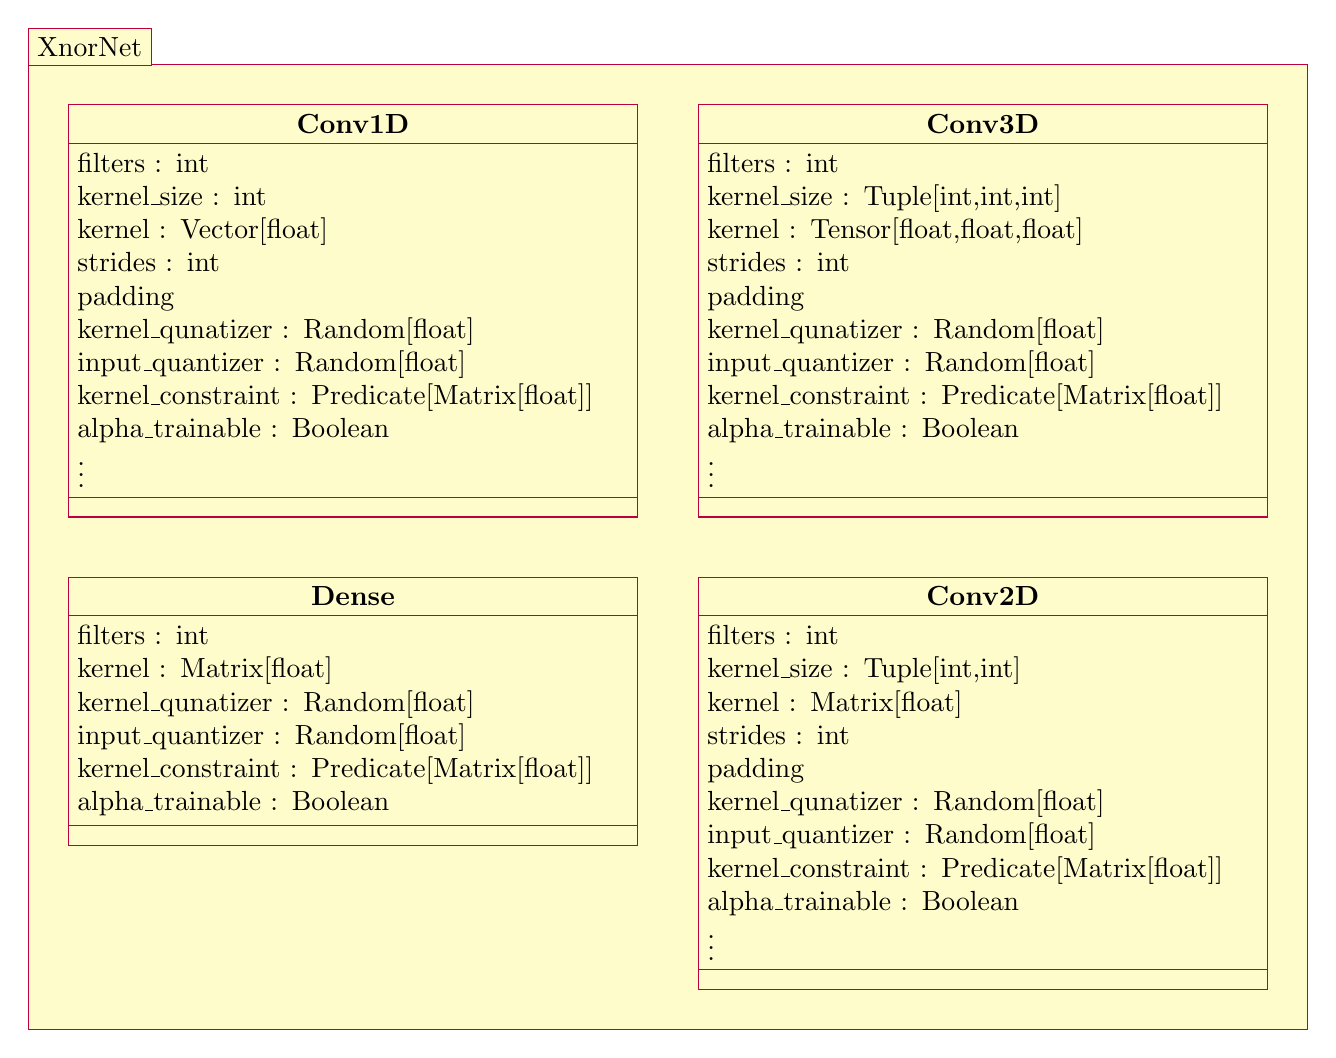
\begin{tikzpicture}
		\begin {package}{XnorNet}
		\begin {class}[text width= 7cm ]{Dense}{0, 0}
		\attribute{filters : int}
		\attribute{kernel : Matrix[float]}
		\attribute{kernel\_qunatizer : Random[float]}
		\attribute{input\_quantizer : Random[float]}
		\attribute{kernel\_constraint : Predicate[Matrix[float]]}
		\attribute{alpha\_trainable : Boolean}
		\vdots
	\end{class}
	\begin {class}[text width= 7cm ]{Conv1D}{0 ,6cm}
	\attribute{filters : int}
	\attribute{kernel\_size : int}
	\attribute{kernel : Vector[float]}
	\attribute{strides : int}
	\attribute{padding}
	\attribute{kernel\_qunatizer : Random[float]}
	\attribute{input\_quantizer : Random[float]}
	\attribute{kernel\_constraint : Predicate[Matrix[float]]}
	\attribute{alpha\_trainable : Boolean}
	\attribute{\vdots}
\end{class}
\begin {class}[text width= 7cm ]{Conv2D}{8cm ,0}
\attribute{filters : int}
\attribute{kernel\_size : Tuple[int,int]}
\attribute{kernel : Matrix[float]}
\attribute{strides : int}
\attribute{padding}
\attribute{kernel\_qunatizer : Random[float]}
\attribute{input\_quantizer : Random[float]}
\attribute{kernel\_constraint : Predicate[Matrix[float]]}
\attribute{alpha\_trainable : Boolean}
\attribute{\vdots}
\end{class}
\begin {class}[text width= 7cm ]{Conv3D}{8cm ,6cm}
\attribute{filters : int}
\attribute{kernel\_size : Tuple[int,int,int]}
\attribute{kernel : Tensor[float,float,float]}
\attribute{strides : int}
\attribute{padding}
\attribute{kernel\_qunatizer : Random[float]}
\attribute{input\_quantizer : Random[float]}
\attribute{kernel\_constraint : Predicate[Matrix[float]]}
\attribute{alpha\_trainable : Boolean}
\attribute{\vdots}
\end{class}
\end{package}
\end{tikzpicture}
\caption{XnorNet}
\end{figure}
\FloatBarrier
\newpage 
\subsection{ABCNet}
Le module \texttt{ABCNet} contient $4$ classes qui sont: \texttt{Dense},\texttt{Conv1D},\texttt{Conv2D} et \texttt{Conv3D}.
\newline Chacune de ces classes est une classe fille de \texttt{tensorflow.keras.Model}. 
\begin{figure}[htp]
	\small
	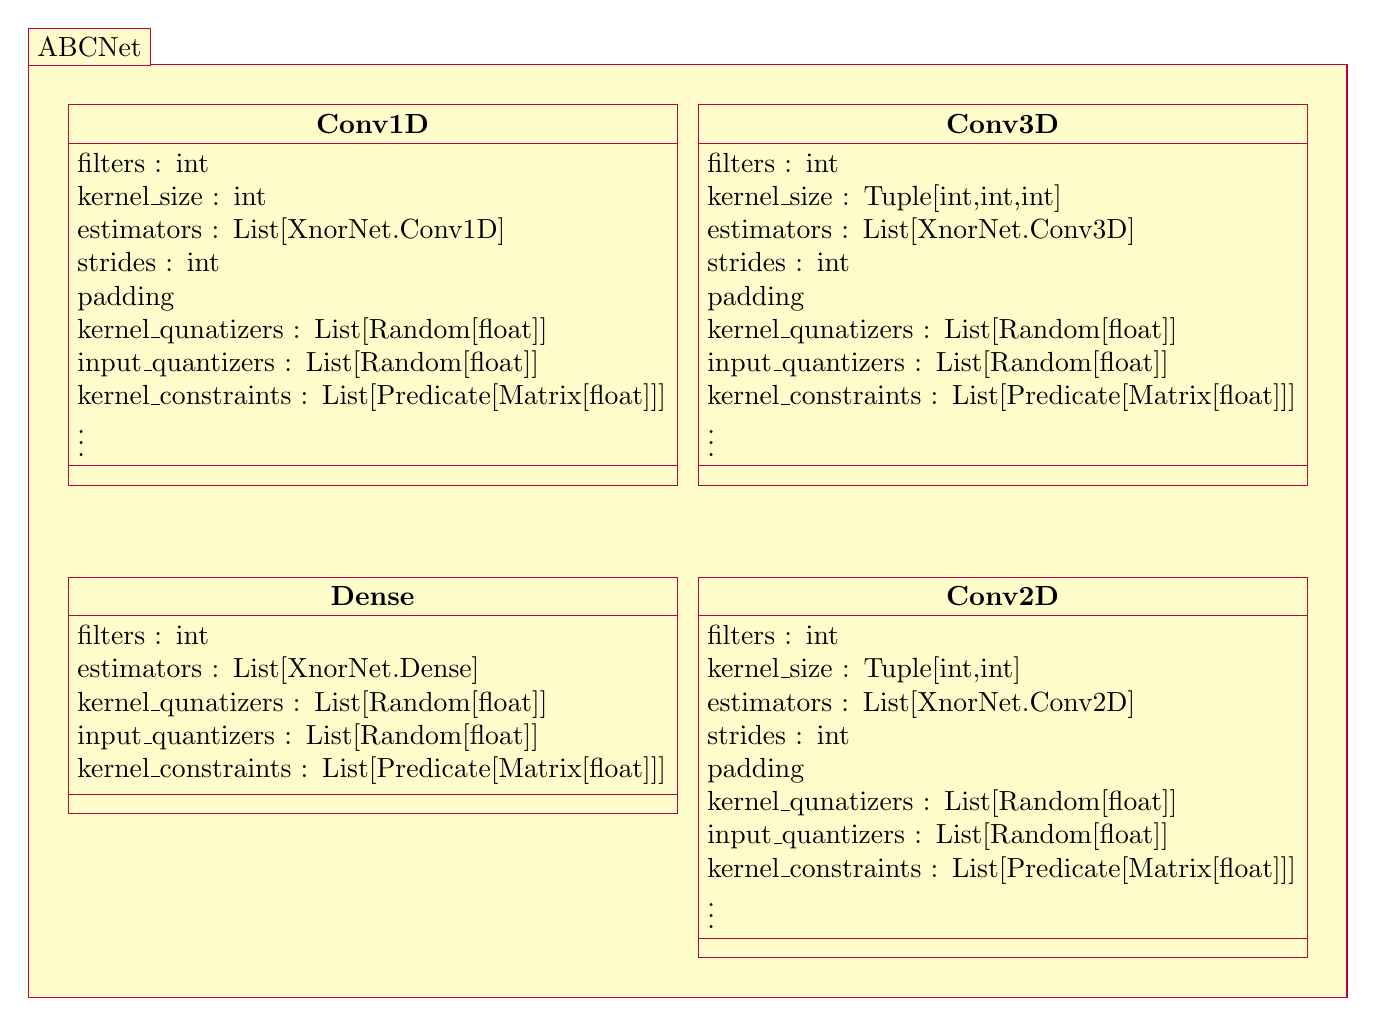
\begin{tikzpicture}
		\begin {package}{ABCNet}
		\begin {class}[text width= 7.5cm ]{Dense}{0, 0}
		\attribute{filters : int}
		\attribute{estimators : List[XnorNet.Dense]}
\attribute{kernel\_qunatizers : List[Random[float]]}
\attribute{input\_quantizers : List[Random[float]]}
\attribute{kernel\_constraints : List[Predicate[Matrix[float]]]}
		\vdots
	\end{class}
	\begin {class}[text width= 7.5cm ]{Conv1D}{0 ,6cm}
	\attribute{filters : int}
	\attribute{kernel\_size : int}
	\attribute{estimators : List[XnorNet.Conv1D]}
	\attribute{strides : int}
	\attribute{padding}
	\attribute{kernel\_qunatizers : List[Random[float]]}
	\attribute{input\_quantizers : List[Random[float]]}
	\attribute{kernel\_constraints : List[Predicate[Matrix[float]]]}
	\attribute{\vdots}
	
\end{class}
\begin {class}[text width= 7.5cm ]{Conv2D}{8cm ,0}
\attribute{filters : int}
\attribute{kernel\_size : Tuple[int,int]}
\attribute{estimators : List[XnorNet.Conv2D]}
\attribute{strides : int}
\attribute{padding}
\attribute{kernel\_qunatizers : List[Random[float]]}
\attribute{input\_quantizers : List[Random[float]]}
\attribute{kernel\_constraints : List[Predicate[Matrix[float]]]}
\attribute{\vdots}
\end{class}
\begin {class}[text width= 7.5cm ]{Conv3D}{8cm ,6cm}
\attribute{filters : int}
\attribute{kernel\_size : Tuple[int,int,int]}
\attribute{estimators : List[XnorNet.Conv3D]}
\attribute{strides : int}
\attribute{padding}
\attribute{kernel\_qunatizers : List[Random[float]]}
\attribute{input\_quantizers : List[Random[float]]}
\attribute{kernel\_constraints : List[Predicate[Matrix[float]]]}
\attribute{\vdots}
\end{class}
\end{package}
\end{tikzpicture}
\caption{ABCNet}
\end{figure}
\FloatBarrier
\newpage
\section{Block}
Ce module est l'implémentation des "couches" des modèles suivant:
\begin{itemize}
	\item BiRealNet
	\item MeliusNet
\end{itemize}
Vue leur nature résiduale, une "couche" de l'un de ces modèles constitute effectivement un bloc.
\begin{remark}
	Ce module n'est nécessaire que dans l'utilisation de l'interface séquentielle.
\end{remark}
Dans ce module, chaque bloc admet un nom de la forme \texttt{NomBloc.TypeCouche} avec:
\begin{itemize}
	\item $\texttt{NomBloc} \in \{\texttt{Sequential},\texttt{BiRealNet},\texttt{MeliusNet}\}$
	\item $\texttt{TypeCouche} \in \{\texttt{Dense},\texttt{Conv1D},\texttt{Conv2D},\texttt{Conv3D}\}$
\end{itemize} 

\begin{figure}[htp]
	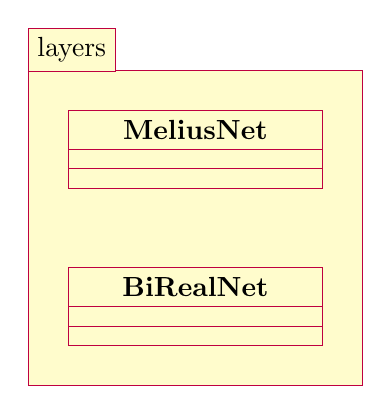
\begin{tikzpicture}
		\begin {package}{layers}
		\begin {class}[text width = 3cm]{BiRealNet}{0, 0}
	\end{class}
	\begin {class}[text width = 3cm]{MeliusNet}{0 ,2cm}
\end{class}
\end{package}
\end{tikzpicture}
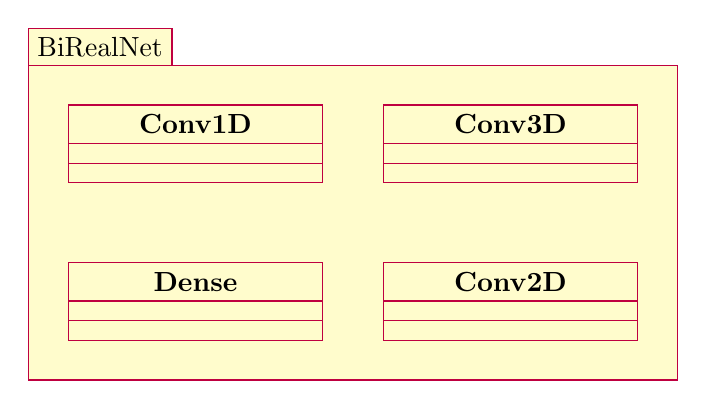
\begin{tikzpicture}
\begin {package}{BiRealNet}
\begin {class}[text width = 3cm]{Dense}{0, 0}
\end{class}
\begin {class}[text width = 3cm]{Conv1D}{0 ,2cm}
\end{class}
\begin {class}[text width = 3cm]{Conv2D}{4cm ,0}
\end{class}
\begin {class}[text width = 3cm]{Conv3D}{4cm ,2cm}
\end{class}
\end{package}
\end{tikzpicture}
\caption{Le contenu de \texttt{blocs}, et de \texttt{BiRealNet}}
\end{figure}
\FloatBarrier

\newpage 
\section{Binarisations}
Dans ce qui précède, nous n'avons parlé que de la fonction signe avec STE dans la propagation en arrière. Mais en effet BinaryFlow, supporte plusieurs binarisations, et ces binarisations peut être utilisés dans n'importe quel couche grâce à l'aspect modulaire.
\newline Pour chaque binarisation, on peut aussi personnaliser l'estimation de son gradient, ce qui donne une flexibilité dans le choix de la binarisation. 
\newline Pour cela, nous allons étudier les binarisations que nous avons implémentés, et les approximations de leurs gradients
\subsection{Propagation en Avant}
\begin{definition}
	Une méta-binarisation est un opérateur $\mathcal{K}$ qui prends une binarisation $\Psi$ et donne une autre binarisation $\mathcal{K}(\Psi)$
\end{definition}
Nous avons les binarisations suivantes
\subsubsection{Fonction signe}
L'expression de cette fonction est:
\begin{equation}
	x\rightarrow \sign (x)
\end{equation}
\subsubsection{Fonction heavyside}
L'expression de cette fonction est:
\begin{equation}
	x\rightarrow H (x)
\end{equation}
Cette binarisation doit être utilisé avec attention, car son utilisation rend plusieurs formules \\ analytiques de XnorNet et ABCNet invalides.
\begin{figure}[htp!]
	\centering
	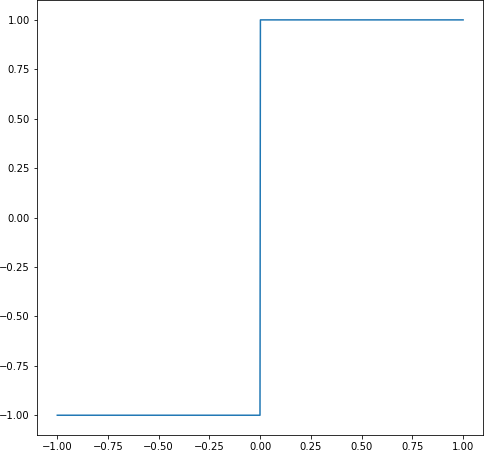
\includegraphics[width=0.4\textwidth]{Figures/sign-cropped.png}
	\caption{Traçage des fonction Signe et Heaviside}
	\label{fig:Sign-Heaviside}
\end{figure}
\FloatBarrier
\subsubsection{Binarisation décalée}
C'est une meta-binarisation qui prend une binarisation $\Psi$ et donne $\Psi$ décalé par un paramètre $\mu:$
\begin{equation}
	x\rightarrow \Psi(x+\mu)
\end{equation}
\begin{figure}[htp]
	\centering
	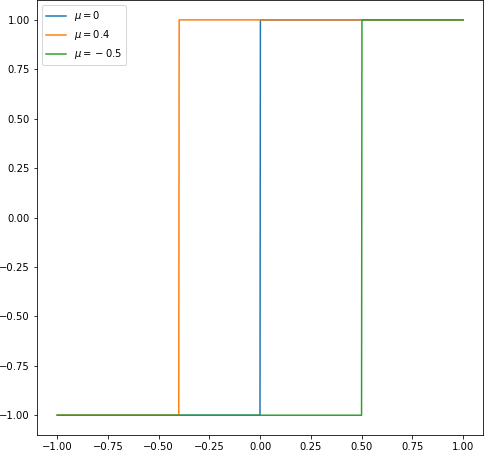
\includegraphics[width=0.33\textwidth]{Figures/shifted-sign-cropped.png}
	\caption{Traçage de la fonction signe décalée à gauche par $\mu$}
	\label{fig:ShiftedSign}
\end{figure}
\FloatBarrier
Le paramètre $\mu$ peut être fixe ou entraîné.
\subsubsection{Binarisation stochastique}
C'est aussi une meta-binarisation. Elle prend une binarisation $\Psi$ et donne $\Psi$ décalé par une variable aléatoire $z$
\begin{equation}
	x\rightarrow \Psi(x+z)
\end{equation}
\begin{figure}[htp]
	\centering
	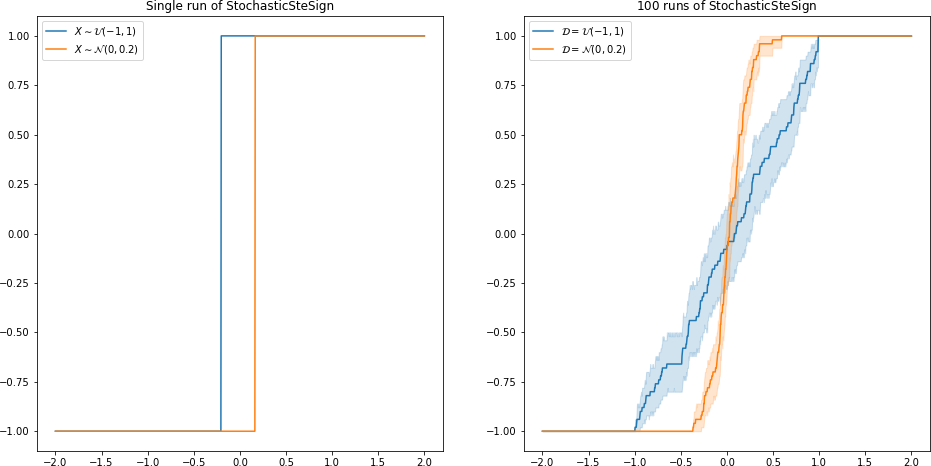
\includegraphics[width=0.66\textwidth]{Figures/stochastic-sign-cropped.png}
	\caption{Traçage de la fonction signe stochastique}
	\footnotesize
	Dans cette figure, $\mathcal{N}(0,0.2)$ dénote la distribution normale centrée avec une deviation standard $\sigma=0.2$, et $\mathcal{U}(-1,1)$ dénote la distribution uniforme dans l'interval $[-1,1]$
	\label{fig:StochasticSign}
\end{figure}
\FloatBarrier
\begin{itemize}
	
	\item La variable aléatoire $z$ suit une distribution $\mathcal{D}$ qui peut être fixe, ou même entraînée.  
	\item Cette binarisation peut être utilisé comme une forme de régularisation pour le modèle.
\end{itemize}

\newpage 
\subsection{Propagation en arrière}
On peut résumer les approximation du gradient par:
\begin{table}[h]
	\small
	\begin{tabularx}{\textwidth}{| p{3cm} | p{3cm} | X |}
		\hline
		
		Estimation & Expression & Binarisation correspende  \\
		\hline 
		STE & $\mathtt{1}_{\lvert x  \rvert} \le 1 $ &  Signe, Heavyside. \\
		\hline  
		ApproxSign & $\mathtt{1}_{\lvert x  \rvert \le 1}  \cdot (2-\lvert x \rvert) $ &  Sign\\
		\hline
		SwishSigne & $\frac{\beta \left(2-\beta x \tanh(\frac{\beta x }{2})\right)}{1+\cosh(\beta x)}$ &  Signe. \\
		\hline 
	\end{tabularx}
	\caption{Les Les estimations de gradient présentes}
\end{table}
\subsection{Implémentation}
Dans binaryflow, les binarisations sont implémentés dans le module \texttt{quantizers}
\newline Toute binarisation implémentée hérite de la classe \texttt{larq.quantizers.Quantizer}, et elle admet aussi un attribut de classe \texttt{precision} qui est égal à $1.$ 
\newline Cet attribut permet à Larq de faire les optimisations adéquates dans la phase de déploiement.
\begin{figure}[htp]
	\small
	\centering
	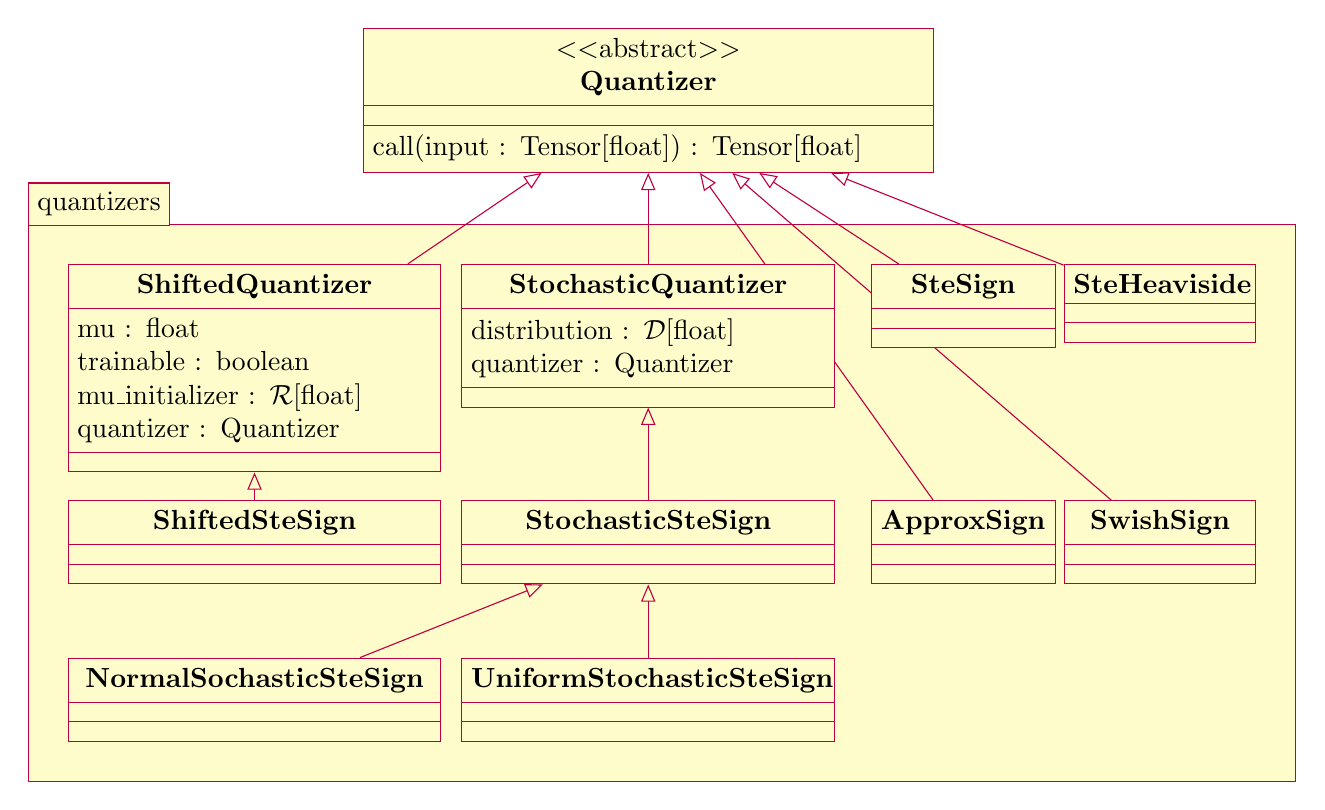
\begin{tikzpicture}
		\begin{abstractclass}[text width=7cm]{Quantizer}{5cm,3cm}
			\operation{call(input : Tensor[float]) : Tensor[float]}
		\end{abstractclass}
		\begin {package}{quantizers}
		\begin {class}[text width = 4.5cm]{ShiftedQuantizer}{0, 0}
		\attribute{mu : float}
		\attribute{trainable : boolean}
		\attribute{mu\_initializer : $\mathcal{R}$[float]}
		\attribute{quantizer : Quantizer}
		\inherit{Quantizer}
	\end{class}
	\begin {class}[text width = 4.5cm]{ShiftedSteSign}{0cm ,-3cm}
	\inherit{ShiftedQuantizer}
\end{class}
\begin {class}[text width = 4.5cm]{StochasticQuantizer}{5cm ,0cm}
	\attribute{distribution : $\mathcal{D}$[float]}
	\attribute{quantizer : Quantizer}
\inherit{Quantizer}
\end{class}
\begin {class}[text width = 4.5cm]{StochasticSteSign}{5cm ,-3cm}
\inherit{StochasticQuantizer}
\end{class}
\begin {class}[text width=4.5cm]{NormalSochasticSteSign}{0cm ,-5cm}
\inherit{StochasticSteSign}
\end{class}
\begin {class}[text width = 4.5cm]{UniformStochasticSteSign}{5cm ,-5cm}
\inherit{StochasticSteSign}
\end{class}
\begin {class}[text width = 2.1cm]{SteSign}{9cm ,0cm}
\inherit{Quantizer}
\end{class}
\begin {class}[text width = 2.2cm]{SteHeaviside}{11.5cm ,0cm}
\inherit{Quantizer}
\end{class}
\begin {class}[text width = 2.1cm]{ApproxSign}{9cm ,-3cm}
\inherit{Quantizer}
\end{class}
\begin {class}[text width = 2.2cm]{SwishSign}{11.5cm ,-3cm}
\inherit{Quantizer}
\end{class}
\end{package}
\end{tikzpicture}
\caption{Diagramme de classe global du module \texttt{binaryflow.quantizers}}
\end{figure}
\FloatBarrier
\newpage
\section{Régularisations}
Les BNNs supportent les régularisations offertes par les réseaux de neurones classiques.
\newline De plus, ils supportent une autre forme de régularistion appelée régularisation de quantification, qui est un terme $\mathcal{L}_{\text{quantification}}$ ajouté à la fonction objective pour réduire l'erreur de quantification:
\begin{equation}
	\mathcal{L}=\mathcal{L}_{\text{model}} + \mathcal{L}_{\text{quantification}}
\end{equation}
Le terme $\mathcal{L}_{\text{quantification}}$ comporte une somme pondérée de:
\subsection{Erreur de quantification des noeuds}
C'est égal à 
\begin{equation}
	\mathcal{L}_{\text{weight}}=\sum_{a^{(l)} \text{quantified}} \lVert \tilde{a}^{(l)} - a \rVert_p^p
\end{equation}
\subsection{Erreur de quantification des poids}
C'est égal à 
\begin{equation}
	\mathcal{L}_{\text{input}}=\sum_{\boldsymbol{W}^{(l)} \text{quantified}} \lVert \tilde{\boldsymbol{W}}^{(l)} - \boldsymbol{W}^{(l)} \rVert_p^p
\end{equation}
\subsection{Erreur de quantification de l'opération bilinéaire}
C'est aussi l'erreur de quantification de $z^{(l)}.$ 
\newline Cette erreur est l'erreur la plus importante car elle agit directement sur les performances du modèle.
\newline Elle est égale à:
\begin{equation}
	\mathcal{L}_{\text{output}}=\sum_{\boldsymbol{z}^{(l)} \text{quantified}} \left\lVert \tilde{\boldsymbol{z}}^{(l)} - \boldsymbol{z}^{(l)}  \right\rVert_p^p = \sum \left \lVert \tilde{\boldsymbol{W}}^{(l)} \star \tilde{a}^{(l-1)} - \boldsymbol{W}^{(l)} \star a^{(l-1)} \right\rVert_p^p 
\end{equation}
\chapter{Analyse}

\section{Introduction}

Dans ce chapitre, on va résoudre 3 problèmes en utilisant les approches classiques d'apprentissages profonds, et aussi avec les réseaux de neurones binarisés.
On va essentiellement résoudre:
\begin{enumerate}
	\item Régression de $f:x\rightarrow 2x^2+3x+2$ sur $[-4,4]$
	\item Classification des chiffres en exploitant le jeu de données MNIST
	\item Classification des chiffres en exploitant le jeu de données Free Spoken Digits
\end{enumerate} 
\newpage
\section{Méthodologie adoptée}
Dans les problèmes, qui se suivent, nous avons suivi la méthodologie CRSIP-DM\cite{11}.
\subsection{CRISP-DM}
CRISP-DM signifie Cross Industry Standard Process for Data Mining (CRISP-DM) est une méthode mise à l'épreuve sur le terrain permettant d'orienter les travaux d'exploration de données. 
\subsubsection{Cycle CRISP-DM}

\begin{enumerate}
	\item Connaissance du métier.
	\item Connaissance des données.
	\item Préparation des données.
	\item Modélisation des données.
	\item Évaluation.
	\item Déploiement.
\end{enumerate}
\begin{figure}[h!]
	\centering
	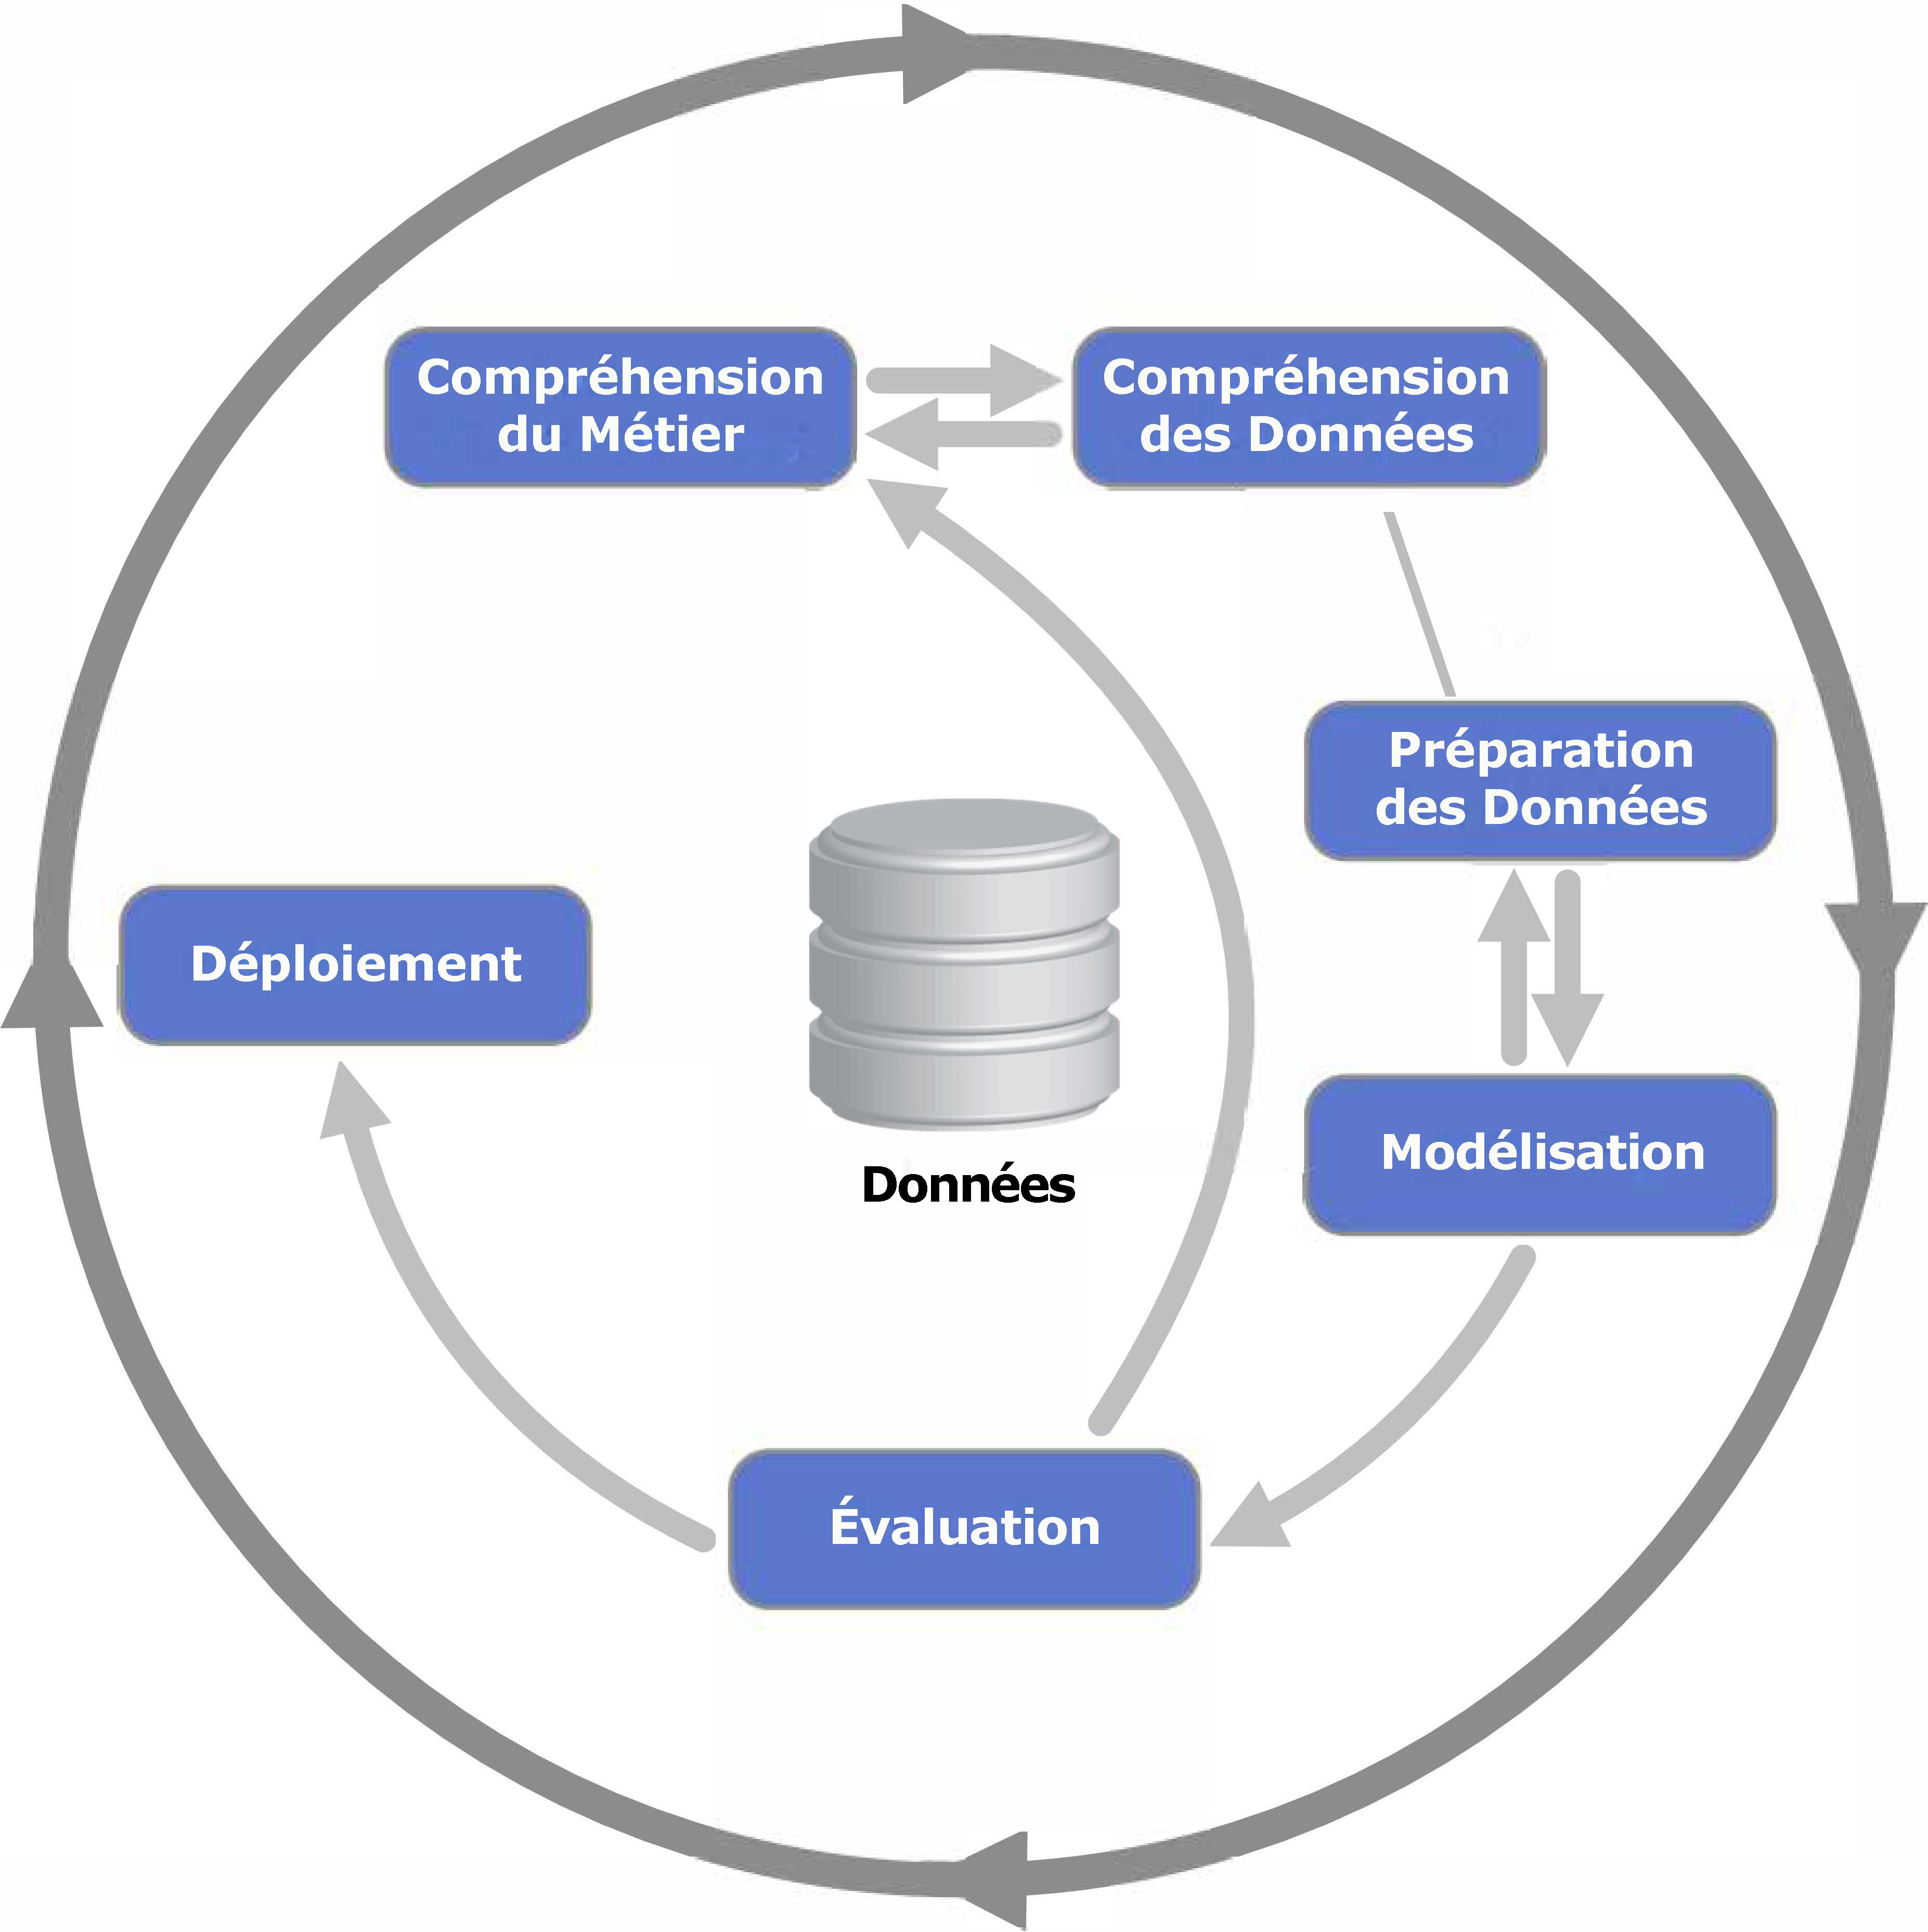
\includegraphics[width=.5\textwidth]{Figures/CRISP-DM.png}
	\caption{Méthodologie CRISP-DM}
	\label{fig:CRSIP-DM}
\end{figure}
\FloatBarrier
\newpage
\section{Régression de $f:x\rightarrow 2x^2+3x+2$ sur $[-4,4]$}
\subsection{Importance}
Ce problème est fait artificiellement étudier la robustesse les  BNNs implémentées.
\subsection{Jeux de données}
Dans cette problématique, le jeu de données est généré avec $n=20000$ exemplaires:
\begin{itemize}
	\item $x_1,\dots,x_n \sim \mathcal{U}(-4,4)$ 
	\item $\epsilon_1,\dots,\epsilon_n \sim \mathcal{N}(0,0.1)$
	\item $y_1,\dots,y_n$ avec $y_i=f(x_i)+\epsilon_i\quad \forall i\in\{1,\dots,n\}.$ 
\end{itemize}

\subsection{Modèle}
Notre modèle $\mathcal{M}_\theta$ est un estimateur de $f$ paramétrisé par $\theta\in S$. L'ensemble $S$ va dépendre de type du modèle.
\newline
Dans notre cas, l'architecture du modèle est décrite par la figure ci-dessous.

Pour la binarisation, nous avons utilisé la fonction $\sign$ dans la propagation avant, et nous avons utilisé la méthode STE bornée sur $[-1,1]$ pour la propagation en arrière.

\subsection{Hypothèses}
On a fait les hypothèses suivantes:
\begin{enumerate}
	\item H1: $x_1,\dots,x_n$ sont mutuellement indépendents
	\item H2: Les bruits sont mutuellement indépendentes.
	\item H3: Le model $\mathcal{M}$ ne connaît sur la fonction $f$ que $f(x_i)\approx y_i,$et il ne tient pas compte de l'erreur $\epsilon_i.$
\end{enumerate}
\subsection{Problème Formel}
On va chercher $\theta^*$ tel que:
\begin{equation}\label{Regression:MSE}
	\theta^* = \argmin_{\theta \in S } \lVert\boldsymbol{y}-\mathcal{M}_\theta(\boldsymbol{x})\rVert_2^2 =\argmin_{\theta \in S }\sum_{i=1}^n(y_i-\mathcal{M}_\theta(x_i))^2
\end{equation}

\subsection{Entraînement}
On a entraîné 3 types de modèles:
\begin{itemize}
	\item BinaryNet
	\item XnorNet
	\item ABCNet
\end{itemize}
Pour chacun, on a utilisé:
\begin{itemize}
	\item L'optimiseur Adam, avec $\mathtt{learning\_rate}=10^{-2}$ et $\mathtt{decay}=10^{-4}$
	\item La fonction objective MSE comme décri dans l'équation \eqref{Regression:MSE}
	\item Taille de lot égale à $128$
	\item Une limite de $30$ époches.
	.
\end{itemize}
\subsection{Performances de prédiction}
On a tracé la courbe de chaque modèle en le comparant avec $f$:
\begin{figure}[h!]
	\centering
	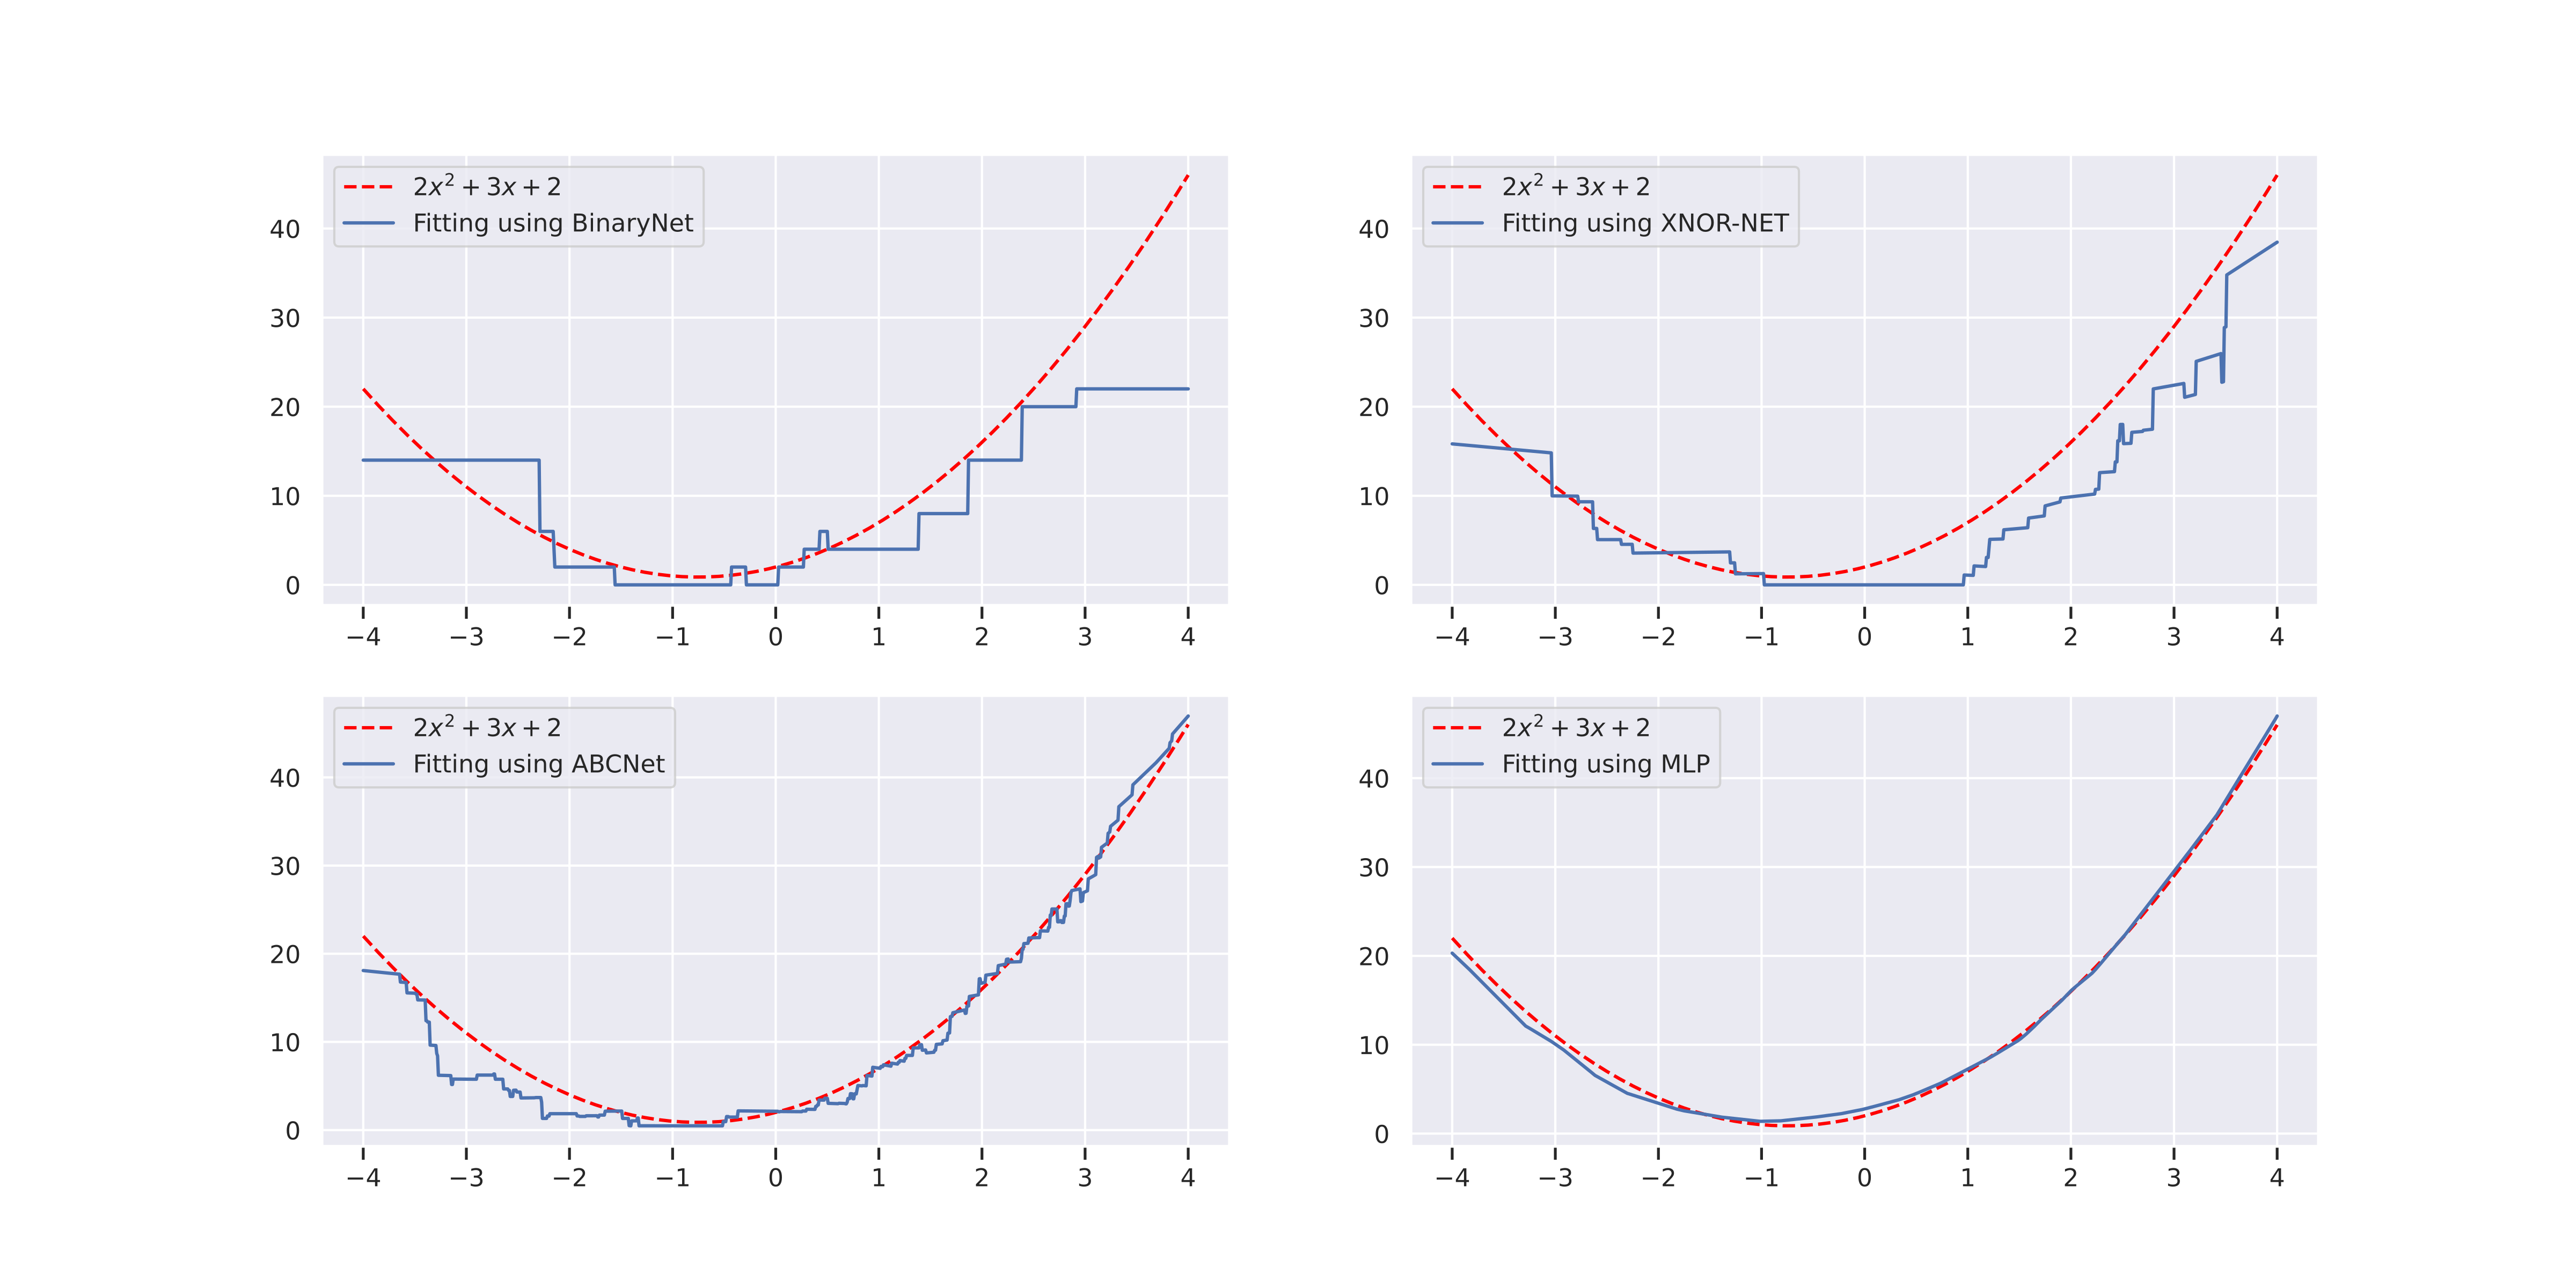
\includegraphics[width=1\textwidth]{Figures/RegressionPerformance.png}
	\caption{Courbe de chaque modèle}
	\label{fig:Regression-Curve}
\end{figure}
\FloatBarrier
Pour mesurer la qualité de régression, nous avons utilisé 3 métriques:
\subsubsection{Distance $\mathscr{L}^\infty$}
C'est la distance $\mathscr{L}^\infty$ dans l'espace des fonctions continues $\mathscr{C}([-4,4])$:
\begin{equation}
	\mathscr{L}^\infty_{\text{test}}(y,\mathcal{M}_\theta)=\sup_{x\in[-4,4]}\lvert \mathcal{M}_\theta(x)-f(x) \rvert
\end{equation}
\subsubsection{Distance $\mathscr{L}^1$}
C'est la distance $\mathscr{L}^1$ dans l'espace $\mathscr{C}([-4,4])$:
\begin{equation}
	\mathscr{L}^1_{\text{test}}(y,\mathcal{M}_\theta)=\int_{-4}^4 \lvert\mathcal{M}_\theta(x)-f(x)\rvert dx
\end{equation}
\subsubsection{Distance $\mathscr{L}^2$}
C'est la distance $\mathscr{L}^2$ dans l'espace $\mathscr{C}([-4,4])$:
\begin{equation}
	\mathscr{L}^2_{\text{test}}(y,\mathcal{M}_\theta)=\left(\int_{-4}^4 \left(\mathcal{M}_\theta(x)-f(x\right))^2 dx\right)^{\frac{1}{2}}
\end{equation}
Dans la pratique, nous allons estimer les 2 intégrales en utilisant la méthode Romb avec $n=2^{20}+1$ points.
\newline 
On a trouvé les résultats suivant:
\newline

\begin{tabularx}{\textwidth}{| X | X | X | X | X |}
	\hline
	
	Modèle & $\mathscr{L}^\infty$ & $\mathscr{L}^1$ & $\mathscr{L}^2$ Carré & $\mathscr{L}^2$  \\
	\hline
	BinaryNet & 24.000 & 4.322 & 42.524 & 6.521 \\
	\hline 
	XNOR-NET & 13.852 & 3.531 & 19.671 & 4.435 \\
	\hline
	ABCNet & 7.395 & 1.421 & 4.024 & 2.01 \\
	\hline
	MLP & 1.692 & 0.616 & 0.562 & 0.750 \\
	\hline
\end{tabularx}
Dans le tableau ci-dessus, MLP est le modèle classique sans utilisation de binarisations, et il sert comme reférence.

\FloatBarrier
\newpage
\section{Classification MNIST}
\subsection{Introduction}
MNIST\cite{12} est un jeu de données des images de chiffres écrits à la main. Il admet:
\begin{itemize}
	\item $60000$ exemplaires pour l'entraînement
	\item $10000$ exemplaires pour le test.  
\end{itemize}
Les images sonts de tailles $28\times 28$ et en niveau de gris, dans lesquels les chiffres sont centrés.

Ce jeu de données sert comme un test de performance des modèles de Machine Learning.

\begin{figure}[h!]
	\centering
	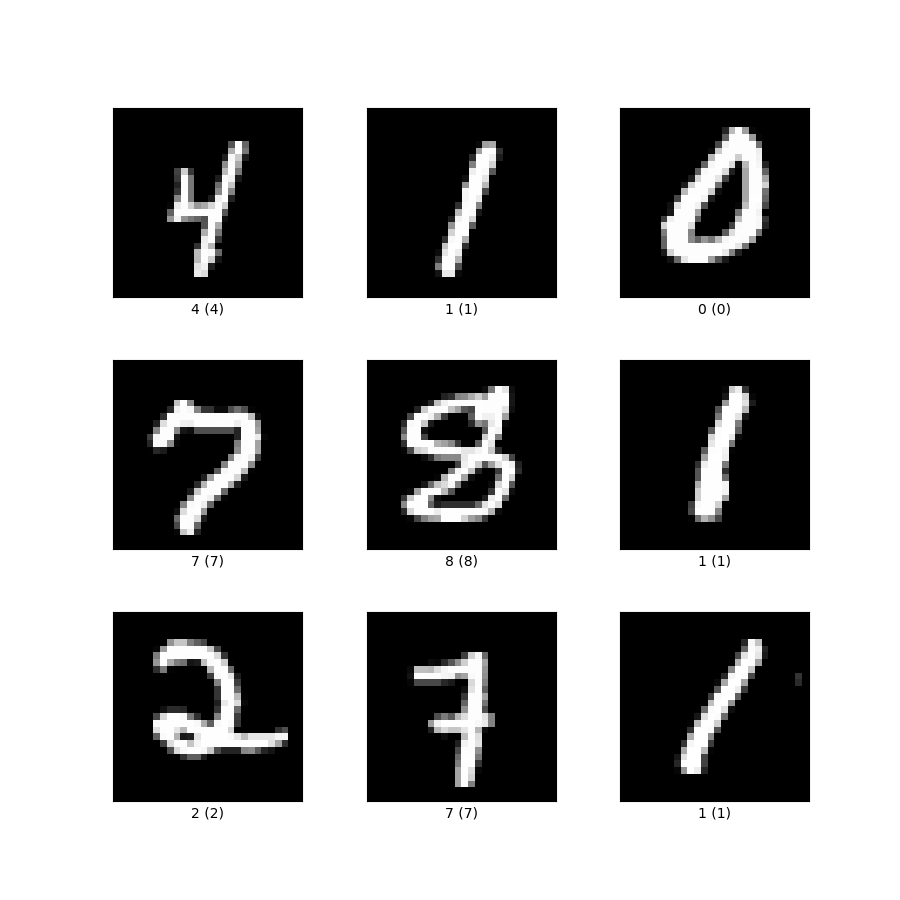
\includegraphics[width=.4\textwidth]{Figures/mnist-3.0.1.png}
	\caption{Des images de MNIST}
	\label{fig:MNIST-Sample}
\end{figure}

\subsection{Topologie}
Nous avons utilisé l'architecture ci-dessous:
\begin{figure}[h!]
	\centering
	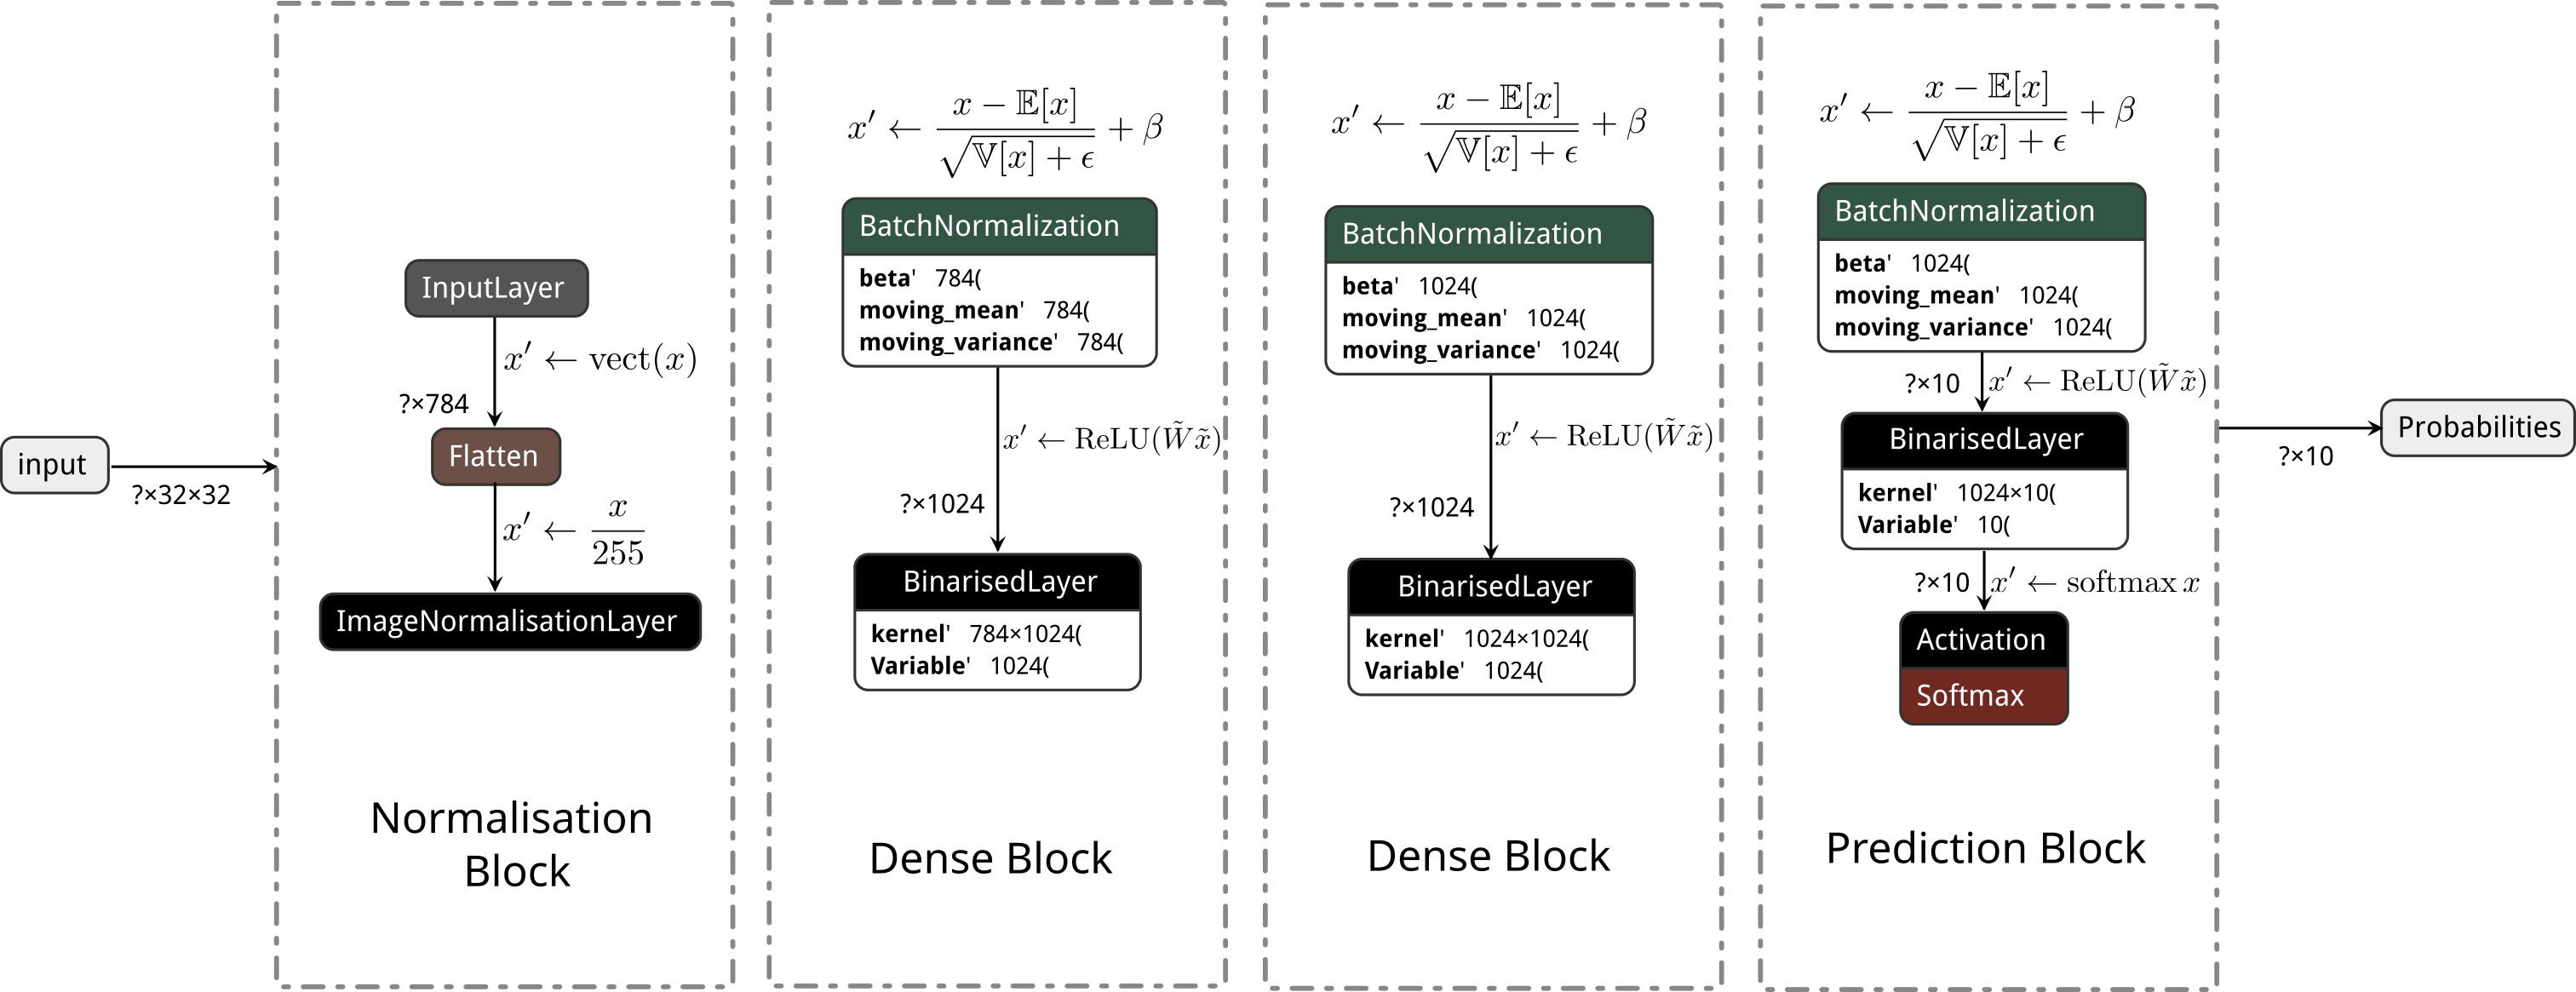
\includegraphics[width=1\textwidth]{Figures/MNIST-Topology.png}
	\caption{Architecture du modèle MNIST}
	\label{fig:MNIST-Topology}
\end{figure}
\FloatBarrier
BinarisedLayer désigne ici le type de couche dense binariséé qui est utilisé. Il s'agit de:
\begin{itemize}
	\item QuantDense pour BinaryNet
	\item ScaledQuantDense pour XnorNet
	\item ABCDense pour ABCNet
\end{itemize}
Dans la figure, les dimensions de couche sont décrits explicitement avec leurs équations, et le point d'interrogation '?' indique que le modèle est indifférent à la taille de lot.
\subsection{Modèle}
On avons utilisé $3$ modèles pour l'architecture donnée:
\begin{itemize}
	\item BinaryNet, avec:
	\subitem Binarisation: $\sign$ avec STE
	\subitem Activation: ReLU
	\item XnorNet, avec:
	\subitem Binarisation: $\sign$ avec STE
	\subitem Activation: ReLU
	\subitem $\alpha$ et $\beta$ sont calculés par produit scalaire.
	\subitem Le facteur $\alpha$ est entraînable, initialisé à \eqref{XnorNet:InnerProductQuantification:Result}
	\subitem Le facteur $\beta$ est calculé, initialisé à \eqref{XnorNet:InnerProductQuantification:Result}
	\item ABCNet avec:
	\subitem Binarisation: $\sign$ décalée avec STE.
	\subitem Activation: ReLU.
	\subitem $n=3$ binarisations des poids, suivant 
	\subitem $m=1$ binarisations des noeuds, suivant
	\subitem $\mu_i$ et $\kappa_j$ sont entraînables
	\subitem $\alpha_i$ et $\beta_j$ sont calculés par produit scalaire.
	
\end{itemize}
\subsection{Performances de prédictions}
\subsection{Performance mémoire}
les performances mémoire sont mésurées avec la taille totale des paramètres, qui donnent une approximation de l'utilisation mémoire du modèle à son déploiement.
\newline Nous avons fait la comparaison de $2$ versions de chaque modèle:
\begin{itemize}
	\item Les paramètres (non-binarisés) sont en float à 32 bits.
	\item Les paramètres (non-binarisés) sont en float à 8 bits.
\end{itemize}
\subsubsection{Comparaison Float 32}
Les paramètres de type float sont naturellement encodés en $64 \ \text{bits}$ dans TensorFlow. En apportant des binarisations, on va avoir le tableau suivant
\begin{table}[h]
	\begin{tabularx}{\textwidth}{| X | X | X | X | X |}
		\hline
		
		Modèle & Nombre de paramètres binarisés &  Nombre de paramètres non-binarisés &  Taille de mémoire en \text{KB} \newline $T$ &  Taux de compression $\tau=\frac{T_{\text{MLP}}}{T_{\text{Model}}}$ \\
		\hline
		MLP & 0 & 1'869'354 & 7302.16 & 1 \\
		\hline 
		BinaryNet & 1'861'632 & 5'664 & 249.38 & 29.28 \\
		\hline
		XnorNet & 1'861'632 & 7'722 & 257.41 & 28.36 \\
		\hline
		ABCNet & 5'584'896 & 11'838 & 727.99 & 10.03 \\
		\hline
	\end{tabularx}
	\caption{Comparaison entre les modèles en utilisant Float32 }
\end{table}
\FloatBarrier
\subsubsection{Comparaison Float 8}
On peut aussi compresser les paramètres float en utilisant Float 8 (Minifloat) dans TensorFlow.
\newline Ainsi, on va avoir le tableau suivant:
\begin{table}[h]
	\begin{tabularx}{\textwidth}{| X | X | X | X | X |}
		\hline
		
		Modèle & Nombre de paramètres binarisés &  Nombre de paramètres non-binarisés &  Taille de mémoire en \text{KB} \newline $T$ &  Taux de compression $\tau=\frac{T_{\text{MLP}}}{T_{\text{Model}}}$ \\
		\hline
		MLP & 0 & 1'869'354 & 7302.16 & 1 \\
		\hline 
		BinaryNet & 1'861'632 & 5'664 & 249.38 & 29.28 \\
		\hline
		XnorNet & 1'861'632 & 7'722 & 257.41 & 28.36 \\
		\hline
		ABCNet & 5'584'896 & 11'838 & 727.99 & 10.03 \\
		\hline
	\end{tabularx}
	\caption{Comparaison entre les modèles en utilisant Float8 }
\end{table}
\FloatBarrier

\subsubsection{Quantification de Float 32 à Float 8}
Avec les deux tableaux précédents, on peut étudier l'apport de la réduction de précision de float à minifloat pour les $4$ modèles considérés en terme de mémoire.
\begin{table}[h]
	\begin{tabularx}{\textwidth}{| X | X | X | X |}
		\hline
		
		Modèle & Taille avec Float 32\newline $T_{32}$ &  Taille avec Float 8  \newline $T_8$&  Rapport de Taille \newline $\tau=\frac{T_{\text{8}}}{T_{\text{32}}}$ \\
		\hline
		MLP & 7302.16 & 1825.54 & 0.25 \\
		\hline 
		BinaryNet & 249.38 & 232.78  & 0.9334 \\
		\hline
		XnorNet & 257.41 & 234.79 & 0.9121 \\
		\hline
		ABCNet & 727.99  & 693.31 & 0.9523\\
		\hline
	\end{tabularx}
	\caption{Comparaison entre les modèles en utilisant Float8 }
\end{table}
\FloatBarrier

\subsection{Performance temps}
les performance temps sonts mésurée avec le nombre d'instructions multiply \& accumulate (MAC) nécessaires pour chaque modèle à son déploiement.


\begin{tabularx}{\textwidth}{| X | X | X | X | X | X |}
	\hline
	
	Modèle & Nombre de MACs binarisés\newline $N_B$ &  Nombre de MACs non-binarisés \newline $$N_F$$ &  Instructions équivalentes: \newline $$I=\frac{N_B}{64}+N_F$$ &  Taux de MACs binarisés \newline $$\alpha=\frac{N_B}{N_B+N_F}$$ & Taux de gain: \newline $$\tau=\frac{I_{\text{MLP}}}{I_{\text{Model}}}$$ \\
	\hline
	MLP & 0 & 1’861’632 & 1’861’632 & 0 & 1 \\
	\hline 
	BinaryNet & 1'861'632 & 2058 & 29'088 & 1 & 64 \\
	\hline
	XnorNet & 1'861'632 & 7'722 & 31'064 & 0.9989 & 59.92 \\
	\hline
	ABCNet & 5'584'896 & 11'838 & 93'438 & 0.9989 & 19.92 \\
	\hline
\end{tabularx}


\newpage
\section{Classification Free Spoken Digits}
\subsection{Importance}
Dans la littérature, les BNNs utilisés principalement avec les jeux de données images. Ainsi, notre objectif est l'utilisation d'un BNN pour résoudre les problèmes de traitement des signaux à faible complexité.
\newline Nous avons choisis Free Spoken Digits\cite{13} comme une preuve de concept de l'applicabilité des BNNs dans ce genre de problèmes. De plus, nous allons utiliser l'expertise de dB Sense pour extraire intelligemment les informations utiles d'une parole afin de construire un classificateur performant et à faible complexité. 
\subsection{Introduction}
Free Spoken Digits\cite{13} (FSD) est un jeu de données audio qui consiste d'un ensemble de fichiers wav à une fréquence d'échantillonage de $8 \ \text{kHz}$. Les fichiers sont coupés pour minimiser le silence.
\begin{figure}[h!]
	\centering
	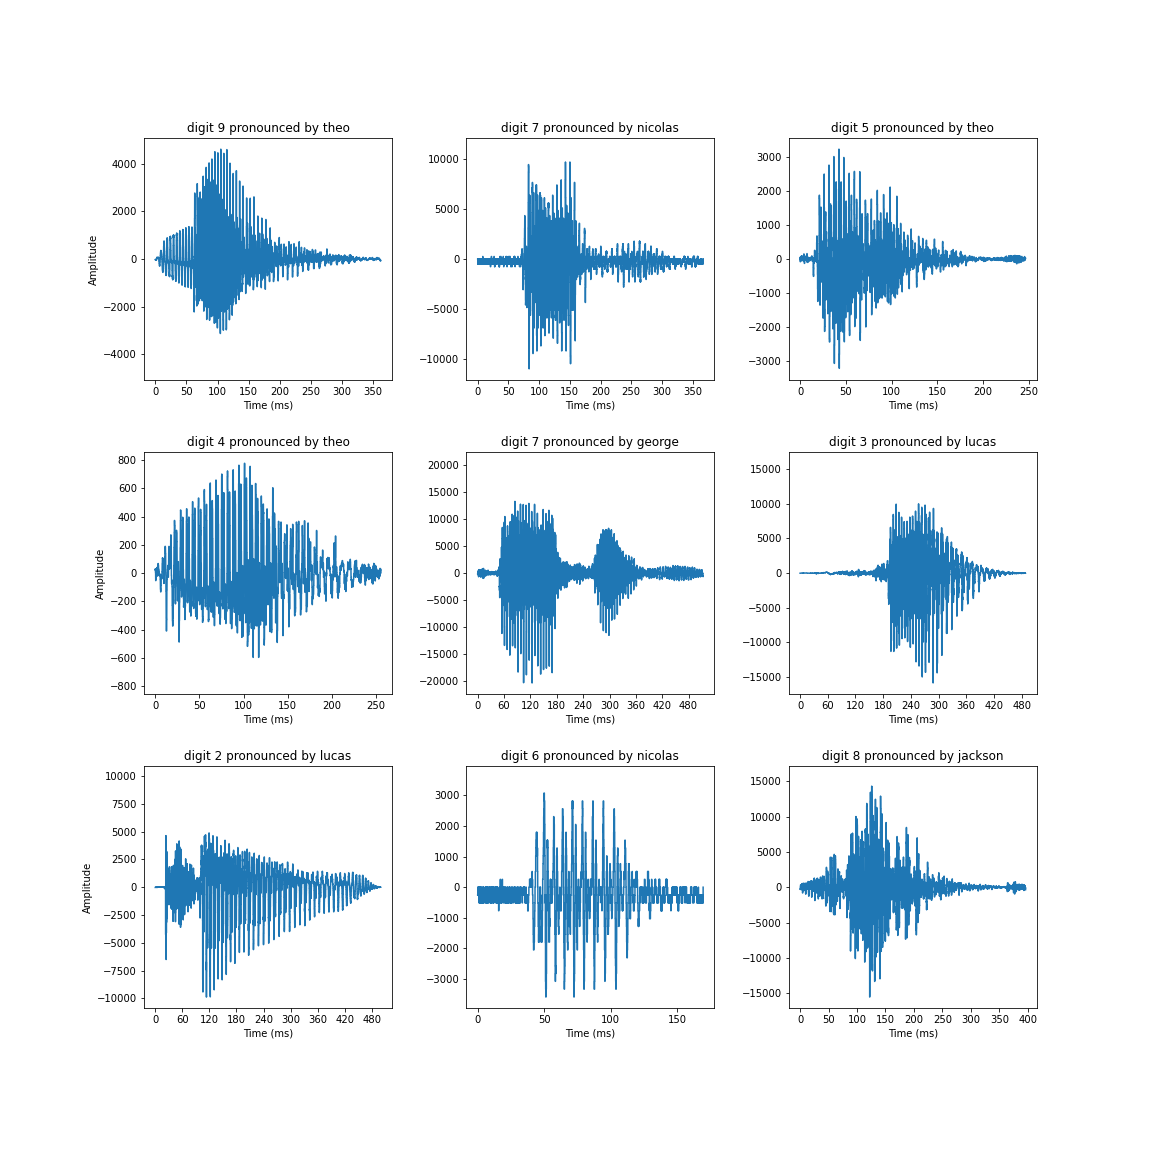
\includegraphics[width=.7\textwidth]{Figures/free-spoken-digits-4.png}
	\caption{Des images de MNIST}
	\label{fig:FreeSpokenDigits-Sample}
\end{figure}
\newpage
\subsection{Structure}
FSD est enrigistré à l'aide d'un microphone monophonique, et il admet $6$ orateurs qui ont chacun $50$ enregistrements par chiffre.
\newline En total, chaque orateur admet $500$ enregistrements, et donc ce jeux de données admet $3000$ fichiers audio.
\newline De plus, chaque enregistrement admet un nom significatif de la forme \texttt{digit\_person\_id.wav} avec:
\begin{itemize}
	\item \texttt{digit} est le chiffre prononcé dans l'enregistrement.
	\item \texttt{person} est le nom de l'orateur.
	\item \texttt{id} est l'identificateur de l'enregistrement, sachant la personne et le chiffre, appartenant à l'ensemble $\{0,\dots,49\}$
\end{itemize}
\subsection{Analyse}

\chapter{Déploiement}

\section{Methodology}
For the machine learning model creation we followed the Knowledge Discovery in Databases (\textit{KDD})\cite{3} methodology which is an iterative multi-stage process for extracting useful information from databases. This process is a road map with multiple stages that emphasises on early decisions and choices we make showing how important planning can lead to a successful and well managed project. This methodology was invented by Oussama Fayyad back in the 1996.

\begin{figure}[h!]
    \centering
    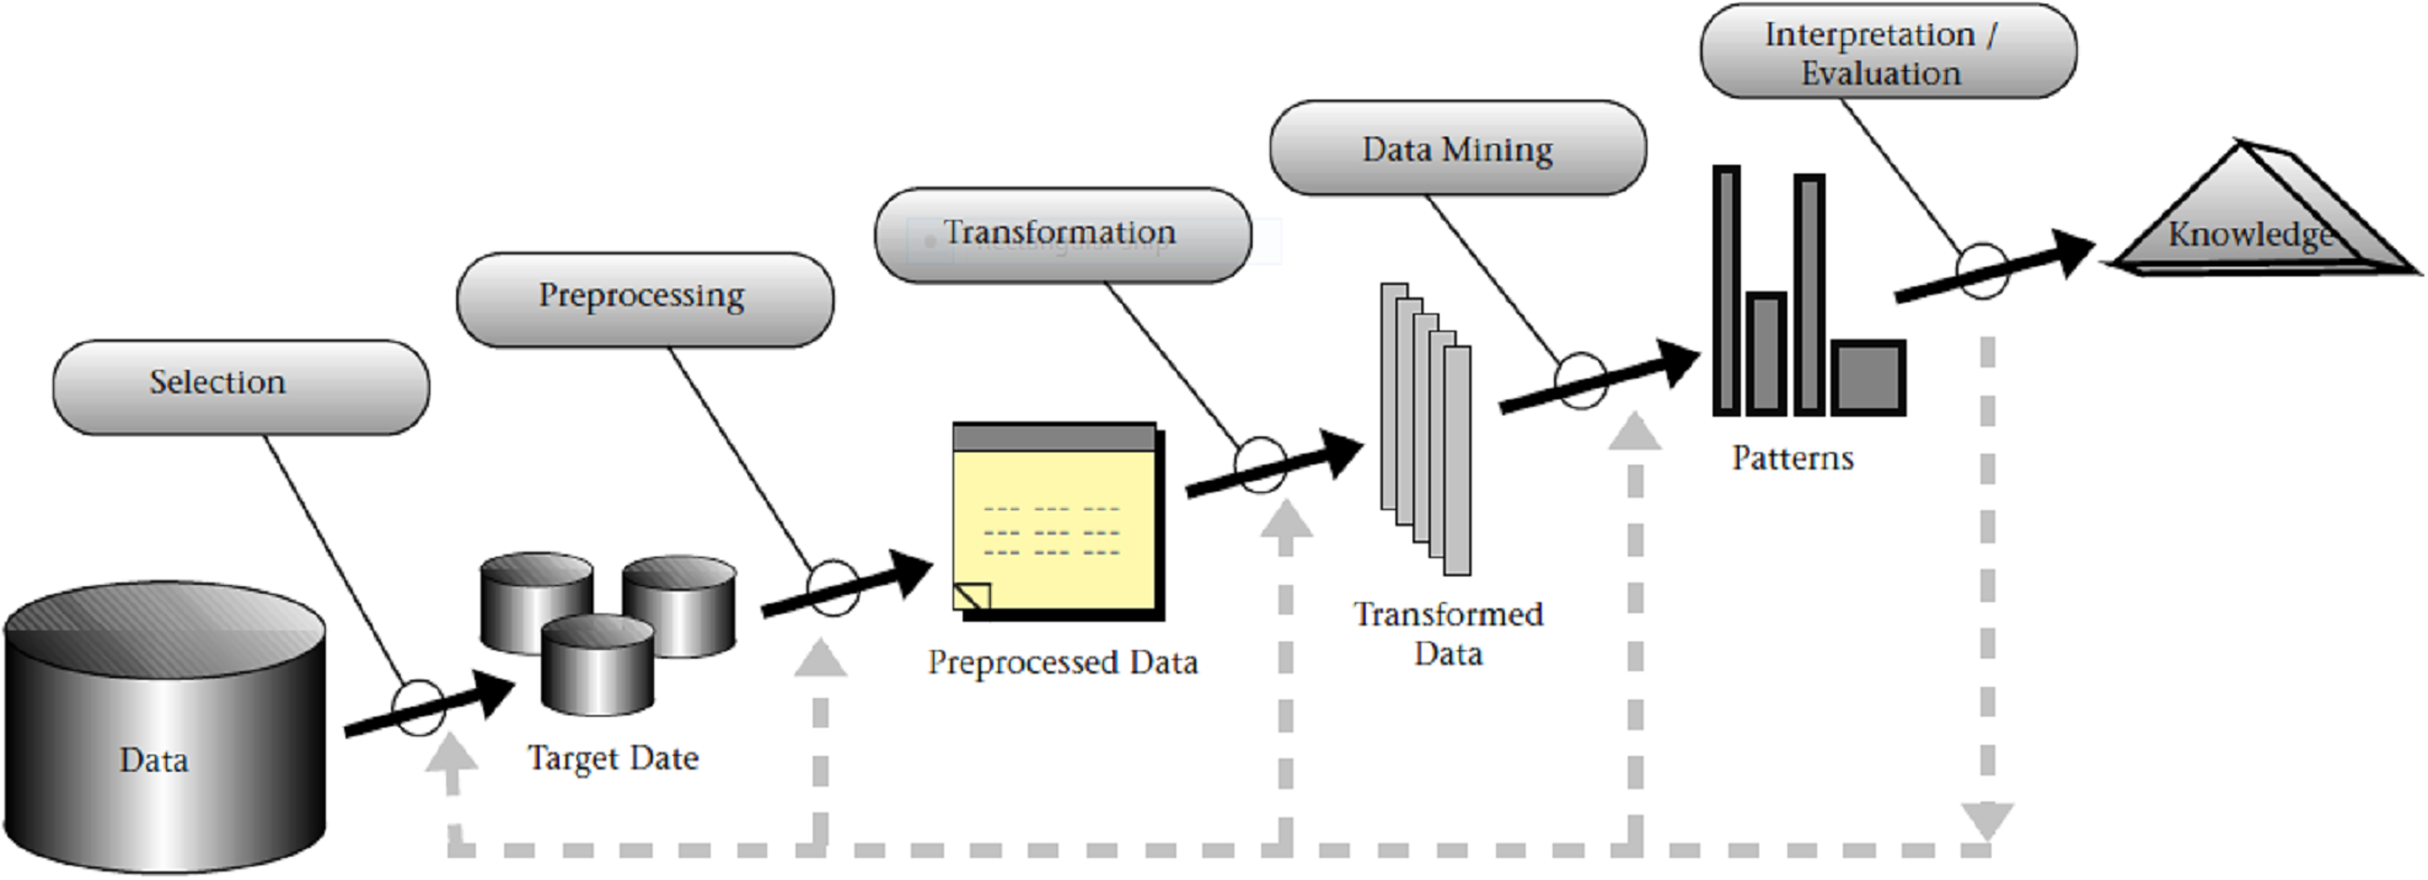
\includegraphics{chapters/KDD.png}
    \caption{Knowledge Discovery in Databases Methodology}
    \label{fig:Knowledge Discovery in Databases Methodology}
\end{figure}

\clearpage

\subsection{Selection}

The initial graphs were gathered from the \href{https://networkrepository.com}{network repository} . In addition to the different characteristics of each graph.
\\
\\
We then used these graphs to run our work product on different environments, gather the results of each test and save them into different files using the \textit{Writer} module.
\\
\\
We also gathered the characteristics from each machine to be used in our model.
\\
\\
\begin{figure}[h!]
    \centering
    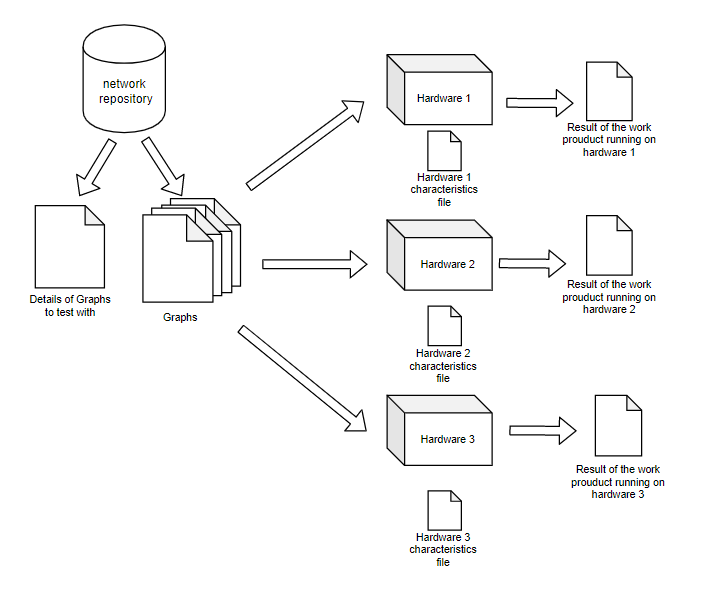
\includegraphics{chapters/Selection.png}
    \caption{Selection stage}
    \label{fig:Selection stage}
\end{figure}
\FloatBarrier
\subsection{Preprocessing and feature selection}

\subsubsection{Data integration}

After the selection phase, we joined our results into one data store from which we are going to extract knowledge.
\\
\\
We joined files containing details on graphs and files containing results of our work product by graph name.
\\
\\
We joined files containing information of the hardware characteristics and our result files by hardware name.
\begin{figure}[h!]
    \centering
    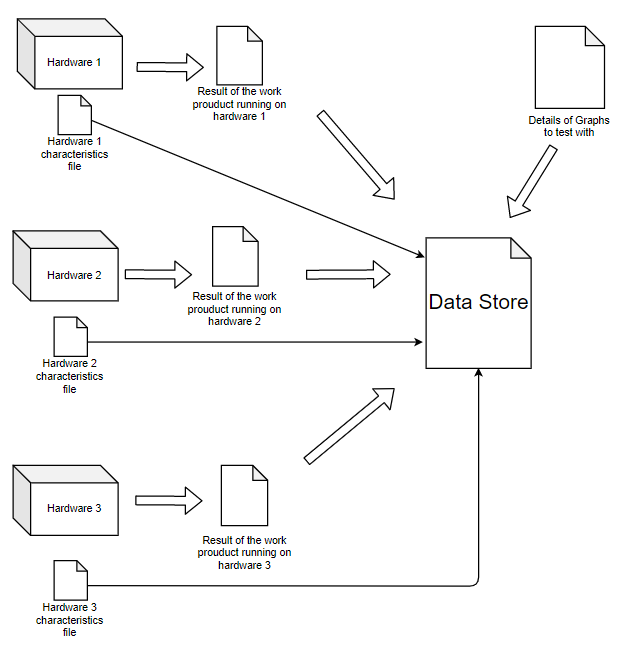
\includegraphics{chapters/merge data.png}
    \caption{Data integration}
    \label{fig:Data integration}
\end{figure}
\FloatBarrier

\subsubsection{Naming conventions}

We started by naming our different features using a certain convention ( all our features are written in \textit{Pascal Case} with spaces between words. Each column not following this convention will be renamed.

\subsubsection{Dividing features based on complexity}

After naming our features we started classifying them based on their complexity. We divided our features into three groups

\begin{itemize}
    \item Available features : these are features that can be easily determined and are generally gathered from our initial data set, such as :
    \begin{itemize}
        \item \textit{Number Of Threads}: This feature is used implicitly by the Graph Strategy prediction model 
        \item \textit{Number Of Edges $\lvert\mathcal{E}\rvert$}: This can be calculated by only counting the lines on the file, and can even be estimated in $\mathcal{O}(1)$ by viewing the graph file size and reading some random lines.
        \item \textit{Number Of Nodes $\lvert\mathcal{V}\rvert$}: We set $n\leftarrow 0$, we then read each vertex $u$ on the file, and set $n\leftarrow \max(n,u+1).$ The number of nodes is then $n$
        \item \textit{Density}:It is equal to $\frac{\lvert\mathcal{E}\rvert}{\lvert\mathcal{V}\rvert(\lvert\mathcal{V}\rvert-1)}$

    \end{itemize}
    \item Calculable features : these features can be calculated from the graph file without creating the graph, such as : 
        \begin{itemize}
            \item Contains all Available features.
            \item \textit{Max Degree}: This can be calculated by creating a vector of size $\lvert\mathcal{V}\vert$ and for each line $u \quad v$ of the graph file we set $T[u]\leftarrow T[u]+1.$ the max degree is then $\max_{u} T[u]$
            \item \textit{Min Degree}: Same as the max degree, but we return $\min_{u} T[u]$
            \item \textit{Average Degree}: Same as the max degree, but we return $\frac{\sum_u T[u]}{\lvert\mathcal{V}\rvert}$
    \end{itemize}
    \item Hard features : These are features requires the creation of the graph, or are simply computationally not feasible, such as :
    \begin{itemize}
        \item \textit{Assortativity}
        \item \textit{Number Triangles}: The fastest possible algorithm\cite{8} has complexity $\mathcal{O}(\lvert \mathcal{V}\rvert ^\omega)$\footnote{$\omega\approx 2.376$ is the fast matrix multiplication exponent.}.So it is not feasible to calculate the number of triangles given the size of considered graphs, we can only do some estimations of this features.
        \item \textit{Average Number Of Triangles}, \textit{Max Number Of Triangles}, \textit{Average Clustering Coefficient}, \textit{Fraction Closed Triangles}: Are all directly related to the number of triangles, so they share its computational complexity.
        \item \textit{Max K Core}: can be calculated in linear time $\mathcal{O}(\lvert\mathcal{V}\rvert+\lvert\mathcal{E}\rvert),$ but only if the graph is created, which is not possible in our case, because we are going to estimate the best strategy without creating the graph itself!. 
    
    \end{itemize}
\end{itemize}

\subsubsection{Imputing memory missing values}

By knowing at least the result when we run our test on a specific hardware with a graph using a fixed number of threads, we can predict the ram usage of other test results on the same hardware and same graph using linear regression with a good precision. This has been observed initially in the previous chapter.
\\
\\
For that reason, we will complete missing memory values using linear regression for each graph and hardware couple, these diagrams represent that process : 

\begin{figure}[h!]
    \centering
    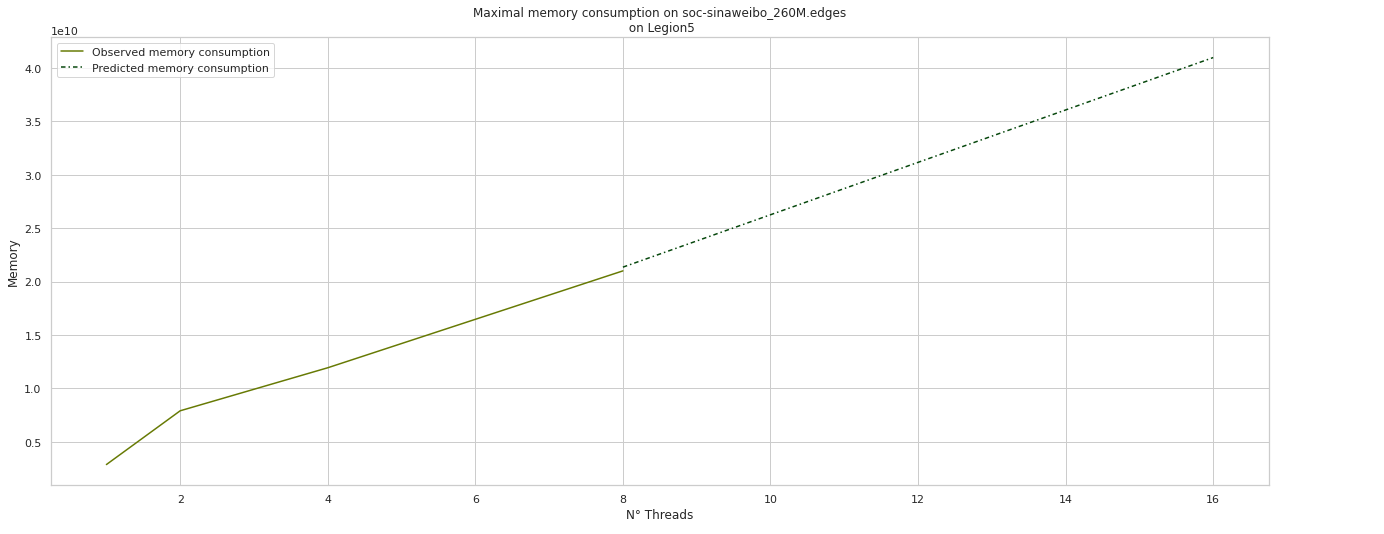
\includegraphics[width=1.0\textwidth]{images/260_legion5.png}
    \caption{Linear regression on ideapad machine}
    \label{fig:Linear regression on ideapad machine}
\end{figure}


\begin{figure}[h!]
    \centering
    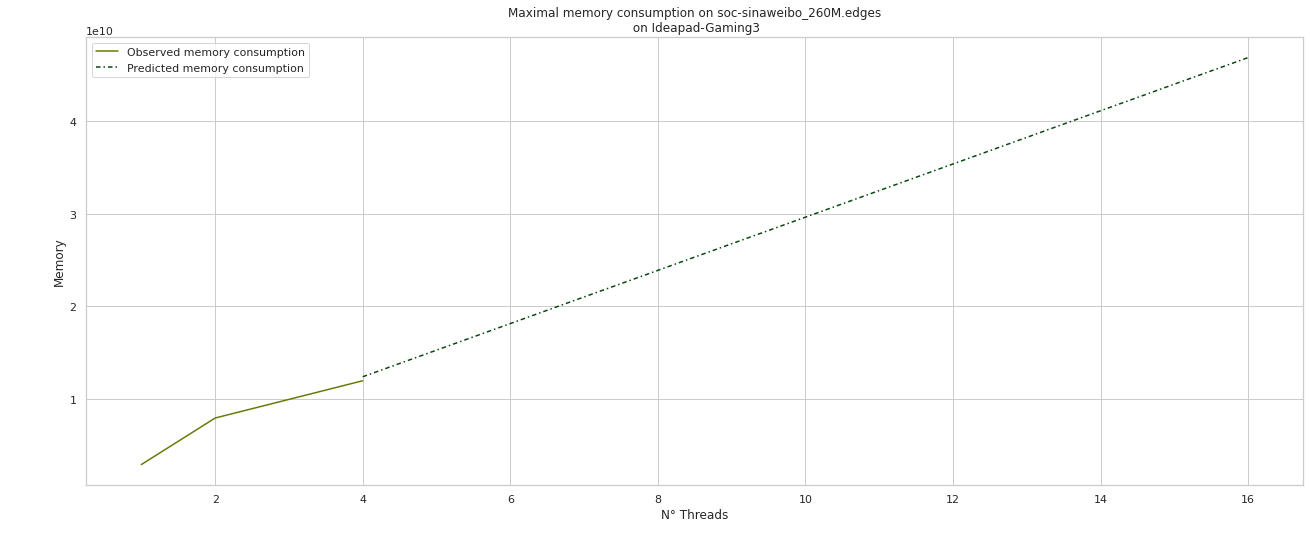
\includegraphics[width=1.0\textwidth]{images/260_ideapad.png}
    \caption{Linear regression on legion5 machine}
    \label{fig:Linear regression on legion5 machine}
\end{figure}

\subsection{Transformation}

In this step we transformed a few of our values to ensure easier manipulation and readability later on.  
    \begin{itemize}
        \item we converted all time fields into \textit{seconds}
        \item we converted the memory to \textit{Gigabyte}
    \end{itemize}

\subsection{Data Mining}

\subsubsection{Data Mining Memory and time}

We started by building two models. One to predict the approximate time the graph creation and the other to predict the memory used. These models will later be used in our final model to predict the best number of threads we can use.

\subsubsection{Predicting number of threads that maximizes memory usage}

Having the Time Model and the memory model, we can now search for the optimal number of threads that minimizes the graph creation time without exhausting the memory. So we created a Graph Strategy Prediction model that predicts the number of threads using the following algorithm:
\\
\\

\begin{algorithm}
\caption{Number of threads prediction}\label{alg:cap}
    \begin{algorithmic}
        \State $nbThreadsBest \gets 1$
        \State $timeUsedMin \gets +\infty$
        \While{$nbThreads \leq limit$}
            \State $memoryUsed \gets memoryModel(nbThreads)$
            \State $timeUsed \gets timeModel(nbThreads)$
            \If{$timeUsed < timeUsedMin$}
                \If {$MemoryUsed < memoryLimit$}
                    \State $timeUsedMin \gets timeUsed$
                    \State $nbThreadsBest \gets nbThreads$
                \EndIf
            \EndIf
        \EndWhile
    \end{algorithmic}
\end{algorithm}


\subsection{Model Selection}
Initially We selected the following $4$ models: 
\begin{itemize}
\item Linear Support vector Machine:  It gives us the flexibility to define how much error is acceptable in our model and will find an appropriate line (or hyperplane in higher dimensions) to fit the data.
\item Linear Regression: The model tries to fit the data into one linear function and make certain predictions based on that linear function.
\item Decision tree: is a model that generates a tree that represents rules to make certain predictions.
\item Random Forest: is an ensemble learning method based on decision tree which is derived from the bagging method to reduce the over-fitting of the decision tree model. 
\end{itemize}

Also We will consider the following $3$ feature sets:
\begin{itemize}
    \item Available Features
    \item Calculable Features
    \item Calculable + Hard Features 
\end{itemize}

Which will give us $3\times 4=12$ possible models. We will then test the performance of each one.

\section{Results}
As we are following the KDD methodology, and as we selected and preprocessed our data set now we are going to select features that we are going to work with, so initially we are going to use Available features then we evaluate the model performance and we go back to the data mining stage to select other set of features (Calculable features and Calculable + Hard features). Mainly, we implemented two testing methods : 


\subsection{Train test split}
As a first estimation of the model performance, we used Train Test split technique.
Here we split our data set into Train and Test data sets with 70\% for the train set and 30\% for the test set. The performance indicator is $\mathcal{R}^{2}$\cite{10} :

\begin{table}[ht]
    \centering
    \begin{tabularx}{\textwidth}{| X |  X | X | X |}
        \hline
        & Available Features &  Calculable Features & Calculable + Hard Features \\
		\hline
        LinearSVR              & 0.391       & 0.515        &   0.447    \\ \hline
        LinearRegressor        & 0.398       & 0.642        &   0.554    \\ \hline
        DecisionTreeRegressor  & 0.943       & 0.986        &   0.934    \\ \hline
        RandForestRegressor    & 0.926       & 0.965        &   0.988    \\ \hline
    \end{tabularx}
    \caption{Using train test split validation on memory models}
\end{table}


\begin{table}[ht]
    \centering
    \begin{tabularx}{\textwidth}{| X |  X | X | X |}
        \hline
        & Available Features &  Calculable Features & Calculable + Hard Features \\
		\hline
        LinearSVR              & 0.531    & 0.606   &   0.578  \\ \hline
        LinearRegressor        & 0.595    & 0.655   &   0.645  \\ \hline
        DecisionTreeRegressor  & 0.958    & 0.927   &   0.947  \\ \hline
        RandForestRegressor    & 0.936    & 0.977   &   0.975  \\ \hline
    \end{tabularx}
    \caption{Using train test split validation on time models}
\end{table}

We can observe that two tree based models (Decision Tree and Random Forest) performed better than the other two models (Linear Regression and Support Vector Machine). This has to do with the fact that the latter are both geometric models\footnote{Which supposes that the input features are members of a Hilbert/Euclidean Space}, but in fact our features do not have a geometric interpretation.

\subsection{Cross Validation}

As the results show, we got a very high model performance, which led us to suspect that our model is experiencing data leakage\footnote{Data Leakage\cite{9} is a situation in machine learning and statistics on which the given (training) data contains unexpected extra information about the subject it is estimating.}. So to have a better estimation of the error, we Used cross validation with \textbf{10 folds}. These are our results for the different models tested : 



\begin{table}[ht]
    \centering
    \begin{tabularx}{\textwidth}{| X |  X | X | X |}
        \hline
        & Available Features &  Calculable Features &  Calculable + Hard Features \\
		\hline
        LinearSVR              & 0.355       & 0.293        &   0.296     \\ \hline
        LinearRegressor        & -3.465      & -2.475       &   -2.524    \\ \hline
        DecisionTreeRegressor  & 0.750       & 0.899        &   0.897     \\ \hline
        RandForestRegressor    & 0.838       & 0.934        &   0.939     \\ \hline
    \end{tabularx}
    \caption{Using 10-fold cross validation on memory models}
\end{table}


\begin{table}[ht]
    \centering
    \begin{tabularx}{\textwidth}{| X |  X | X | X |}
        \hline
        & Available Features &  Calculable Features & Calculable + Hard Features \\
		\hline
        LinearSVR              & -1.164    & -1.207   &   -2.064  \\ \hline
        LinearRegressor        & -5.603    & -3.976   &  -3.886  \\ \hline
        DecisionTreeRegressor  & 0.672     & 0.558    &   0.547  \\ \hline
        RandForestRegressor    & 0.726     & 0.749    &   0.757  \\ \hline
    \end{tabularx}
    \caption{Using 10-fold cross validation on time models}
\end{table}


So we deduce that indeed, there was some leakage from Training set to Testing set, and also the results confirm that the geometric models perform worse than tree based models. 
\\
\\
Also the we can deduce also that the Decision Tree regression model was overfitting, but it was not detected in the Train Test split phase due to data leakage
\\
\\
Finally, while Random Forest was also leaking, it did have better overall performance as Random Forest is more resilient to the over-fitting phenomenon. So our memory and time models will be a \textit{RandomForestRegressor}, using Calculable Features, as it is not practical to extract Hard Features in practice.

\section{Final Model}
Our final model is based on two \textit{RandomForestRegressor}, one for time prediction, and the other for memory prediction, and it predicts the number of threads based on the algorithm described in section $5.1.4$ 

\begin{figure}[h!]
    \centering
    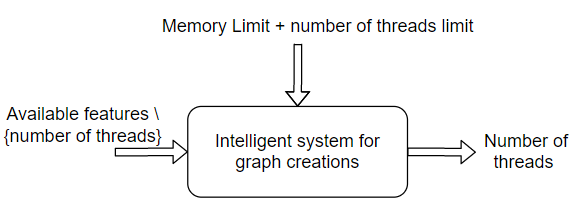
\includegraphics[]{chapters/model.png}
    \caption{Final Model}
    \label{fig:Final Model}
\end{figure}
\FloatBarrier

\section{Conclusion}
In this chapter we presented different stages we went through to create the machine learning models that predict the best strategy to create the graph based on the characteristics of the hardware and details about the graph we want to create. 



\chapter*{Conclusion}
\addcontentsline{toc}{chapter}{Conclusion}

Throughout the preparation of our end-of-year project, we wanted to tackle the graph creation problem using a clear methodology. From evaluating the different strategies and implementations until we eventually build an intelligent model that can predict the best creation strategy.
\\
\\
We started by specifying the context and by modelling our problem mathematically in order to have a clear vision on what we want to build.
\\
\\
In chapter 2, We presented our design and the different design principles we followed in order to ensure the flexibility and resiliency of our work product.
\\
\\
In chapter 3, we presented the different tools used and our general process, in addition to the different challenges we faced while building the Monitoring software that was used later to generate inputs to be used the machine learning phase.
\\
\\
In chapter 4, we analyzed the different results we gathered after we run the software on multiple machines. Which helped later on while building the machine learning pipeline.
\\
\\
And finally, we presented our machine learning methodology, explained in details its different steps and presented the results to get a working intelligent system for graph creation.
\nocite{*}

\printbibliography

\addcontentsline{toc}{chapter}{Bibliography}


\end{document}

% End of document
